\documentclass[11pt]{book}

\usepackage{hypre}
\usepackage{graphicx}
\usepackage[all,cmtip]{xy}
\usepackage[
pdftex,
linktocpage,          % make page numbers be the link on TOC, LOF and LOT
pagebackref,          % adds backlink to the bibliography
plainpages=false,     % page anchors are named by their formatted form
pdfstartview=Fit,     % startup page view
bookmarksopen,        % show bookmarks with all the subtrees expanded
bookmarksopenlevel=0, % open bookmarks only to a certain depth
bookmarksnumbered     % include section numbers in bookmarks
]{hyperref}

% set margins
\setlength{\oddsidemargin}{0in}
\setlength{\evensidemargin}{0in}
\setlength{\textwidth}{6.5in}
\setlength{\topmargin}{0in}
\setlength{\textheight}{8.0in}

% define various commands and macros
\def\pilut{{\sl PILUT}}

% define the version number
% NOTE: this is automatically generated from another file in hypre
\input{version}

% write out the index entries in the `.idx' file
%\makeindex

%=============================================================================
% Body:
%=============================================================================

\begin{document}

%--------------- Title Page

\begin{TitlePage}

\Title{User's Manual}
\SubTitle{Software Version: \HYPREVersion}
\SubTitle{Date: \HYPREVersionDate}
\vfill
\begin{center}

\includegraphics[width=.7\textwidth]{hypre_wiw}
\end{center}
\vfill
\Author{%
Center for Applied Scientific Computing\\
Lawrence Livermore National Laboratory
}

\end{TitlePage}

%--------------- Copyright Page

\begin{CopyrightPage}
\input{copyright.txt}
\end{CopyrightPage}

%--------------- Table of Contents

\pagenumbering{roman}
\tableofcontents
\cleardoublepage
\pagenumbering{arabic}

%--------------- Include Chapters

%=============================================================================
%=============================================================================

\chapter{Introduction}
\label{ch-Introduction}

This manual describes \hypre{}, a software library of high performance
preconditioners and solvers for the solution of large, sparse linear systems of
equations on massively parallel computers \cite{RDFalgout_JEJones_UMYang_2004TA}.  The \hypre{} library was created
with the primary goal of providing users with advanced parallel preconditioners.
The library features parallel multigrid solvers for both structured and
unstructured grid problems.  For ease of use, these solvers are accessed from
the application code via \hypre{}'s conceptual linear system interfaces \cite{RDFalgout_JEJones_UMYang_2005a}
(abbreviated to {\em conceptual interfaces} throughout much of this manual),
which allow a variety of natural problem descriptions.

This introductory chapter provides an overview of the various features in
\hypre{}, discusses further sources of information on \hypre{}, and
offers suggestions on how to get started.

%-----------------------------------------------------------------------------

\section{Overview of Features}
\label{Features}

\begin{itemize}

\item
{\bf Scalable preconditioners provide efficient solution on today's
and tomorrow's systems:} \hypre{} contains several families of
preconditioner algorithms focused on the scalable solution of {\it
very large} sparse linear systems. (Note that small linear systems,
systems that are solvable on a sequential computer, and dense systems
are all better addressed by other libraries that are designed
specifically for them.)
\hypre{} includes ``grey-box'' algorithms
that use more than just the matrix to solve certain classes of
problems more efficiently than general-purpose libraries. This
includes algorithms such as structured multigrid.


\item
{\bf Suite of common iterative methods provides options for a spectrum
of problems:} \hypre{} provides several of the most commonly used
Krylov-based iterative methods to be used in conjunction with its
scalable preconditioners. This includes methods for nonsymmetric
systems such as GMRES and methods for symmetric matrices such as
Conjugate Gradient.

\item
{\bf Intuitive grid-centric interfaces obviate need for complicated
data structures and provide access to advanced solvers:} \hypre{} has
made a major step forward in usability from earlier generations of
sparse linear solver libraries in that users do not have to learn
complicated sparse matrix data structures.  Instead, \hypre{} does the
work of building these data structures for the user through a variety
of conceptual interfaces, each appropriate to different classes of
users.  These include stencil-based structured/semi-structured
interfaces most appropriate for finite-difference applications; a
finite-element based unstructured interface; and a linear-algebra
based interface.  Each conceptual interface provides access to several
solvers without the need to write new interface code.

\item
{\bf User options accommodate beginners through experts:} \hypre{}
allows a spectrum of expertise to be applied by users. The beginning
user can get up and running with a minimal amount of effort. More
expert users can take further control of the solution process through
various parameters.

\item
{\bf Configuration options to suit your computing system:} \hypre{}
allows a simple and flexible installation on a wide variety of
computing systems.  Users can tailor the installation to match their
computing system. Options include debug and optimized modes, the
ability to change required libraries such as MPI and BLAS, a
sequential mode, and modes enabling threads for certain solvers.  On
most systems, however, \hypre{} can be built by simply typing
\kbd{configure} followed by \kbd{make}, or by using CMake \cite{CMakeWebPage}.

\item
{\bf Interfaces in multiple languages provide greater flexibility for
applications:} \hypre{} is written in C (with the exception of the {\tt FEI}
interface, which is written in C++) and utilizes Babel to provide
interfaces for users of Fortran 77, Fortran 90, C++, Python, and Java.
For more information on Babel, see
\url{http://www.llnl.gov/CASC/components/babel.html}.

\end{itemize}



%-----------------------------------------------------------------------------

\section{Getting More Information}

This user's manual consists of chapters describing each conceptual interface, a
chapter detailing the various linear solver options available, and detailed
installation information.  In addition to this manual, a number of other
information sources for \hypre{} are available.

\begin{itemize}

\item
{\bf Reference Manual:} The reference manual comprehensively lists all of the
interface and solver functions available in \hypre{}.  The reference manual is
ideal for determining the various options available for a particular solver or
for viewing the functions provided to describe a problem for a particular
interface.

\item{\bf Example Problems:} A suite of example problems is provided with the
\hypre{} installation.  These examples reside in the \file{examples}
subdirectory and demonstrate various features of the \hypre{} library.
Associated documentation may be accessed by viewing the \file{README.html} file
in that same directory.

\item
{\bf Papers, Presentations, etc.:} Articles and presentations related to the
\hypre{} software library and the solvers available in the library are available
from the \hypre{} web page at \url{http://www.llnl.gov/CASC/hypre/}.

\item{\bf Mailing List:} The mailing list {\sl hypre-announce} can be subscribed
to through the \hypre{} web page at \url{http://www.llnl.gov/CASC/hypre/}.  The
development team uses this list to announce new releases of \hypre{}.  It cannot
be posted to by users.

\end{itemize}

%-----------------------------------------------------------------------------

\section{How to get started}

\subsection{Installing \hypre{}}

As previously noted, on most systems \hypre{} can be built by simply typing
\kbd{configure} followed by \kbd{make} in the top-level source directory.
Alternatively, the CMake system \cite{CMakeWebPage} can be used, and is the best
approach for building \hypre{} on Windows systems in particular.  For more
detailed instructions, read the \file{INSTALL} file provided with the \hypre{}
distribution or refer to the last chapter in this manual.  Note the following
requirements:

\begin{itemize}

\item To run in parallel, \hypre{} requires an installation of MPI.

\item Configuration of \hypre{} with threads requires an implementation
of OpenMP.  Currently, only a subset of \hypre{} is threaded.

\item The \hypre{} library currently does not directly support complex-valued
systems.

\end{itemize}

\subsection{Choosing a conceptual interface}

An important decision to make before writing any code is to choose an
appropriate conceptual interface.  These conceptual interfaces are
intended to represent the way that applications developers naturally
think of their linear problem and to provide natural interfaces for them
to pass the data that defines their linear system into \hypre{}.
Essentially, these conceptual interfaces can be considered convenient
utilities for helping a user build a matrix data structure for
\hypre{} solvers and preconditioners.  The top row of
Figure~\ref{fig-conceptual-interface} illustrates a number of
conceptual interfaces.  Generally, the conceptual interfaces are
denoted by different types of computational grids, but other
application features might also be used, such as geometrical
information.  For example, applications that use structured grids
(such as in the left-most interface in the
Figure~\ref{fig-conceptual-interface}) typically view their linear
problems in terms of stencils and grids.  On the other hand,
applications that use unstructured grids and finite elements typically
view their linear problems in terms of elements and element stiffness
matrices. Finally, the right-most interface is the standard
linear-algebraic (matrix rows/columns) way of viewing the linear
problem.

The \hypre{} library currently supports four conceptual interfaces,
and typically the appropriate choice for a given problem is fairly
obvious, e.g. a structured-grid interface is clearly inappropriate for
an unstructured-grid application.


\begin{itemize}

\item
{\bf Structured-Grid System Interface (\code{Struct}):} This interface is
appropriate for applications whose grids consist of unions of logically
rectangular grids with a fixed stencil pattern of nonzeros at each grid point.
This interface supports only a single unknown per grid point.  See Chapter
\ref{ch-Struct} for details.

\item
{\bf Semi-Structured-Grid System Interface (\code{SStruct}):} This
interface is appropriate for applications whose grids are mostly
structured, but with some unstructured features.  Examples include
block-structured grids, composite grids in structured adaptive mesh
refinement (AMR) applications, and overset grids.  This interface
supports multiple unknowns per cell. See Chapter \ref{ch-SStruct} for details.

\item
{\bf Finite Element Interface (\code{FEI}):} This is appropriate for
users who form their linear systems from a finite element
discretization.  The interface mirrors typical finite element data
structures, including element stiffness matrices.  Though this
interface is provided in \hypre{}, its definition was determined
elsewhere (please email to Alan Williams william@sandia.gov for
more information). See Chapter \ref{ch-FEI} for details.

\item
{\bf Linear-Algebraic System Interface (\code{IJ}):} This is the
traditional linear-algebraic interface.  It can be used as a last
resort by users for whom the other grid-based interfaces are not
appropriate.  It requires more work on the user's part, though still
less than building parallel sparse data structures.  General solvers
and preconditioners are available through this interface, but not
specialized solvers which need more information.  Our experience is
that users with legacy codes, in which they already have code for
building matrices in particular formats, find the IJ interface
relatively easy to use. See Chapter \ref{ch-IJ} for details.

\end{itemize}


\begin{figure}
\centering
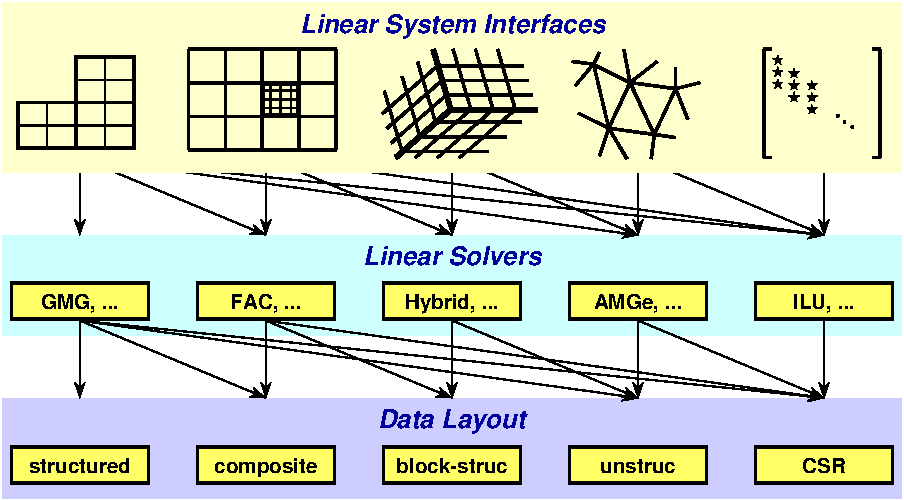
\includegraphics[width=5in]{fig_concep_iface}
\caption{%
Graphic illustrating the notion of conceptual interfaces.}
\label{fig-conceptual-interface}
\end{figure}

Generally, a user should choose the most specific interface that
matches their application, because this will allow them to use
specialized and more efficient solvers and preconditioners without
losing access to more general solvers.  For example, the second row of
Figure~\ref{fig-conceptual-interface} is a set of linear solver
algorithms.  Each linear solver group requires different information
from the user through the conceptual interfaces.  So, the geometric
multigrid algorithm (GMG) listed in the left-most box, for example,
can only be used with the left-most conceptual interface.  On the
other hand, the ILU algorithm in the right-most box may be used with
any conceptual interface.  Matrix requirements for each solver and
preconditioner are provided in Chapter \ref{ch-Solvers} and in the
\hypre{} Reference Manual.  Your desired solver strategy may influence
your choice of conceptual interface.  A typical user will select a
single Krylov method and a single preconditioner to solve their system.


The third row of Figure~\ref{fig-conceptual-interface} is a list of
data layouts or matrix/vector storage schemes.  The relationship
between linear solver and storage scheme is similar to that of the
conceptual interface and linear solver.  Note that some of the
interfaces in \hypre{} currently only support one matrix/vector
storage scheme choice.  The conceptual interface, the desired solvers
and preconditioners, and the matrix storage class must all be
compatible.


%-----------------------------------------------------------------------------

\subsection{Writing your code}

As discussed in the previous section, the following decisions should
be made before writing any code:

\begin{enumerate}
\item Choose a conceptual interface. 
\item Choose your desired solver strategy.
\item  Look up matrix requirements for each solver and preconditioner.
\item Choose a matrix storage class that is compatible with your solvers and
preconditioners and your conceptual interface.
\end{enumerate}

Once the previous decisions have been made, it is time to code your
application to call \hypre{}.  At this point, reviewing the previously
mentioned example codes provided with the \hypre{} library may prove
very helpful.  The example codes demonstrate the following general structure 
of the application calls to \hypre{}:

\begin{enumerate}

\item
{\bf Build any necessary auxiliary structures for your chosen
conceptual interface.} This includes, e.g., the grid and stencil
structures if you are using the structured-grid interface.

\item
{\bf Build the matrix, solution vector, and right-hand-side vector
through your chosen conceptual interface.}  Each conceptual interface
provides a series of calls for entering information about your problem
into \hypre{}.

\item
{\bf Build solvers and preconditioners and set solver parameters
(optional).}  Some parameters like convergence tolerance are the same
across solvers, while others are solver specific.

\item
{\bf Call the solve function for the solver.}

\item
{\bf Retrieve desired information from solver.} Depending on your
application, there may be different things you may want to do with the
solution vector.  Also, performance information such as number of
iterations is typically available, though it may differ from solver to
solver.

\end{enumerate}

The subsequent chapters of this User's Manual provide the details
needed to more fully understand the function of each conceptual
interface and each solver.  Remember that a comprehensive list of all
available functions is provided in the \hypre{} Reference Manual, and
the provided example codes may prove helpful as templates for your
specific application.

%-----------------------------------------------------------------------------

%\section{Code Design}

%In this final section of the introductory chapter, the \hypre{} object
%model is briefly discussed.


%%=============================================================================
%=============================================================================

\chapter{Getting Started}
\label{ch-Getting-Started}

Before writing any code:

\begin{enumerate}

\item
{\bf Choose a conceptual interface (see Sections
\ref{sec-What-are-conceptual-interfaces} and
\ref{sec-Which-conceptual-interface}).}
Generally, the choice is fairly obvious.  A structured-grid interface
is clearly inappropriate for an unstructured-grid application.  It is
desirable to use a more specific interface if appropriate, e.g., the
linear-algebraic interface is usable from any type of grid but will
involve much more user work and prevent access to some
grid-type-specific preconditioners.

\item 
{\bf Choose your desired solver strategy.}  For the typical user, this
will mean a single Krylov method and a single preconditioner.

\item 
{\bf Look up matrix requirements for each solver and preconditioner.}
Each specific solver and preconditioner has requirements from the
input matrix.  This information is provided in several places: Chapter
\ref{ch-Solvers}, the \hypre{} Reference Manual, and
the \hypre{} header files.

\item 
{\bf Choose a matrix class that is compatible with your solvers and
preconditioners and your conceptual interface.}  Note that some of the
interfaces currently only support one matrix class choice.

\end{enumerate}
Once the previous decisions have been made, it is time to code your
application to call \hypre{}:
\begin{enumerate}

\item
{\bf Build any necessary auxiliary structures for your chosen
conceptual interface.} This includes, e.g., the grid and stencil
structures if you are using the structured-grid interface.

\item
{\bf Build the matrix, solution vector, and right-hand-side vector
through your chosen conceptual interface.}  Each conceptual interface
provides a series of calls for entering information about your problem
into \hypre{}.

\item
{\bf Build solvers and preconditioners and set solver parameters
(optional).}  Some parameters like convergence tolerance are the same
across solvers, while others are solver specific.

\item
{\bf Call the solve function for the solver.}

\item
{\bf Retrieve desired information from solver.} Depending on your
application, there may be different things you may want to do with the
solution vector.  Also, performance information such as number of
iterations is typically available, though it may differ from solver to
solver.

\end{enumerate}

%-----------------------------------------------------------------------------

\section{A Simple Example}
\label{sec-Simple-Example}

The following code serves as a simple example of the usage of \hypre{}.  In
this example, the structured-grid interface (discussed in Chapter
~\ref{ch-Struct}) is used to enter the problem into \hypre{}, and the
\code{PFMG} Multigrid solver is used to solve the system.  Since the
structured-grid interface currently only supports one underlying matrix class,
there are no choices to make here.  If we were using the semi-structured grid
interface instead, then we would have to choose between the \code{SStruct} and
\code{ParCSR} matrix classes, depending on the solver we want to use.

This example and all other examples in this manual are written in C,
but \hypre{} also supports Fortran.  See Section
\ref{sec-Fortran} for details.

\begin{display}
\begin{verbatim}

/*-----------------------------------------------------------
 * Set up the grid and stencil
 *-----------------------------------------------------------*/

HYPRE_StructGridCreate(MPI_COMM_WORLD, dim, &grid);
HYPRE_StructGridSetExtents(grid, ilower, iupper);
...
HYPRE_StructGridAssemble(grid);
	
HYPRE_StructStencilCreate(dim, stencil_size, &stencil);
HYPRE_StructStencilSetElement(stencil, 0, offset0);
...

/*-----------------------------------------------------------
 * Set up the matrix, right-hand side, and initial guess
 *-----------------------------------------------------------*/

HYPRE_StructMatrixCreate(MPI_COMM_WORLD, grid, stencil, &A);
HYPRE_StructMatrixInitialize(A);
HYPRE_StructMatrixSetBoxValues(A, ilower, iupper, nelts, elts, Avalues);
...
HYPRE_StructMatrixAssemble(A);

HYPRE_StructVectorCreate(MPI_COMM_WORLD, grid, &b);
HYPRE_StructVectorInitialize(b);
HYPRE_StructVectorSetBoxValues(b, ilower, iupper, bvalues);
...
HYPRE_StructVectorAssemble(b);

HYPRE_StructVectorCreate(MPI_COMM_WORLD, grid, &x);
HYPRE_StructVectorInitialize(x);
HYPRE_StructVectorSetBoxValues(x, ilower, iupper, xvalues);
...
HYPRE_StructVectorAssemble(x);

/*-----------------------------------------------------------
 * Set up the solver
 *-----------------------------------------------------------*/

HYPRE_StructPFMGCreate(MPI_COMM_WORLD, &solver);
HYPRE_StructPFMGSetMaxIter(solver, 50);     	 /* optional */
HYPRE_StructPFMGSetTol(solver, 1.0e-06);    	 /* optional */
HYPRE_StructPFMGSetup(solver, A, b, x);

/*-----------------------------------------------------------
 * Solve the linear system
 *-----------------------------------------------------------*/

HYPRE_StructPFMGSolve(solver, A, b, x);

/*-----------------------------------------------------------
 * Get solution info and free up memory
 *-----------------------------------------------------------*/

HYPRE_StructVectorGetBoxValues(x, ilower, iupper, xvalues);
...

HYPRE_StructPFMGDestroy(solver);
HYPRE_StructGridDestroy(grid);
HYPRE_StructStencilDestroy(stencil);
HYPRE_StructMatrixDestroy(A);
HYPRE_StructVectorDestroy(b);
HYPRE_StructVectorDestroy(x);

\end{verbatim}
\end{display}

%-----------------------------------------------------------------------------

\section{What are conceptual interfaces?}
\label{sec-What-are-conceptual-interfaces}

\begin{figure}
\centering
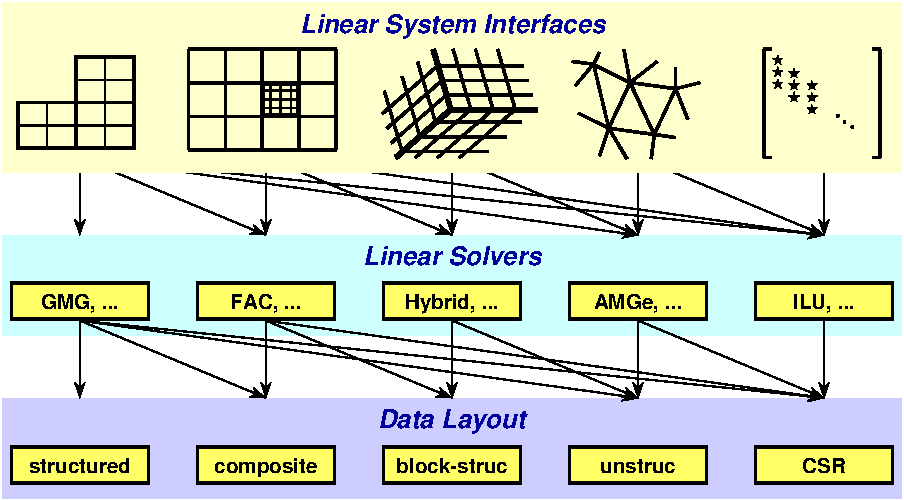
\includegraphics[width=5in]{fig_concep_iface}
\caption{%
Graphic illustrating the notion of conceptual interfaces.
All of these elements are not necessarily in \hypre{}.}
\label{fig-conceptual-interface}
\end{figure}

The top row of Figure~\ref{fig-conceptual-interface} illustrates a number of
conceptual interfaces.  Generally, the conceptual interfaces are denoted by
different types of computational grids, but other application features might
also be used, such as geometrical information.  These conceptual interfaces are
intended to represent the way that applications developers naturally think of
their linear problem, and provide natural interfaces for them to pass the data
that defines their linear system into \hypre{}.  Essentially, these conceptual
interfaces can be considered convenient utilities for helping a user build a
matrix data structure for \hypre{} solvers and preconditioners.  For example,
applications that use structured grids (such as in the left-most interface in
the Figure~\ref{fig-conceptual-interface}) typically view their linear problems
in terms of stencils and grids.  On the other hand, applications that use
unstructured grids and finite elements typically view their linear problems in
terms of elements and element stiffness matrices.  Finally, the right-most
interface is the standard linear-algebraic (matrix rows/columns) way of viewing
the linear problem.

The second row of Figure~\ref{fig-conceptual-interface} is a set of
linear solver algorithms.  Each linear solver group requires different
information from the user through the conceptual interfaces.  So, the
geometric multigrid algorithm (GMG) listed in the left-most box, for
example, can only be used with the left-most conceptual interface.  On
the other hand, the ILU algorithm in the right-most box may be used
with any conceptual interface.

The third row of Figure~\ref{fig-conceptual-interface} is a list of
data layouts or matrix/vector storage schemes.  The relationship
between linear solver and storage scheme is similar to that of
interface and linear solver.

%-----------------------------------------------------------------------------

\section{Which conceptual interface should I use?}
\label{sec-Which-conceptual-interface}

\hypre{} currently supports four conceptual interfaces:

\begin{itemize}

\item
{\bf Structured-Grid System Interface (\code{Struct}):} This interface is
appropriate for applications whose grids consist of unions of logically
rectangular grids with a fixed stencil pattern of nonzeros at each grid point.
This interface supports only a single unknown per grid point.  See Chapter
\ref{ch-Struct} for details.

\item
{\bf Semi-Structured-Grid System Interface (\code{SStruct}):} This
interface is appropriate for applications whose grids are mostly
structured, but with some unstructured features.  Examples include
block-structured grids, composite grids in structured adaptive mesh
refinement (AMR) applications, and overset grids.  This interface
supports multiple unknowns per cell.
See Chapter \ref{ch-SStruct} for details.

\item
{\bf Finite Element Interface (\code{FEI}):} This is appropriate for
users who form their linear systems from a finite element
discretization.  The interface mirrors typical finite element data
structures, including element stiffness matrices.  Though this
interface is provided in \hypre{}, its definition was determined
elsewhere (please email to Alan Williams william@sandia.gov for
more information).  See Chapter \ref{ch-FEI} for details.

\item
{\bf Linear-Algebraic System Interface (\code{IJ}):} This is the
traditional linear-algebraic interface.  It can be used as a last
resort by users for whom the other grid-based interfaces are not
appropriate.  It requires more work on the user's part, though still
less than building parallel sparse data structures.  General solvers
and preconditioners are available through this interface, but not
specialized solvers which need more information.  Our experience is
that users with legacy codes, in which they already have code for
building matrices in particular formats, find the IJ interface
relatively easy to use.
See Chapter \ref{ch-IJ} for details.

\end{itemize}

Generally, a user should choose the most specific interface that
matches their application, because this will allow them to use
specialized and more efficient solvers and preconditioners without
losing access to more general solvers.

%=============================================================================
%=============================================================================

\chapter{Structured-Grid System Interface (Struct)}
\label{ch-Struct}

In order to get access to the most efficient and scalable solvers for
scalar structured-grid applications, users should use the
\code{Struct} interface described in this chapter.  This interface
will also provide access (this is not yet supported) to solvers in
\hypre{} that were designed for unstructured-grid applications and
sparse linear systems in general.  These additional solvers are
usually provided via the unstructured-grid interface (\code{FEI}) or
the linear-algebraic interface (\code{IJ}) described in Chapters
\ref{ch-FEI} and \ref{ch-IJ}.

Figure~\ref{fig-struct-example} gives an example of the type of grid
currently supported by the \code{Struct} interface.  The interface
uses a finite-difference or finite-volume style, and currently
supports only scalar PDEs (i.e., one unknown per gridpoint).
\begin{figure}
\centering
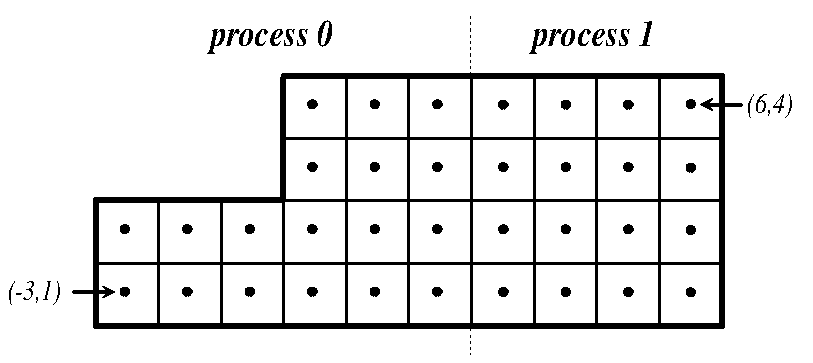
\includegraphics[width=.5\textwidth]{figStructExample1}
\caption{%
An example 2D structured grid, distributed accross two processors.}
\label{fig-struct-example}
\end{figure}
There are four basic steps involved in setting up the linear system
to be solved:
%\begin{enumerate}
\begin{list}{\arabic{enumi}.}{\usecounter{enumi}\setlength{\itemsep}{0in}}
\item set up the grid,
\item set up the stencil,
\item set up the matrix,
\item set up the right-hand-side vector.
\end{list}
%\end{enumerate}
To describe each of these steps in more detail, consider solving the
2D Laplacian problem
\begin{equation}\label{eqn-laplacian}
\left \{
\begin{array}{ll}
\nabla^2 u = f , & \mbox{in the domain}, \\
u = 0,           & \mbox{on the boundary}.
\end{array}
\right .
\end{equation}
Assume (\ref{eqn-laplacian}) is discretized using standard 5-pt finite-volumes
on the uniform grid pictured in \ref{fig-struct-example}, and assume that the
problem data is distributed across two processes as depicted.

%-----------------------------------------------------------------------------

\section{Setting Up the Struct Grid}
\label{sec-Struct-Grid}

The grid is described via a global {\em index space}, i.e., via integer singles
in 1D, tuples in 2D, or triples in 3D (see Figure~\ref{fig-struct-boxes}).
\begin{figure}
\centering
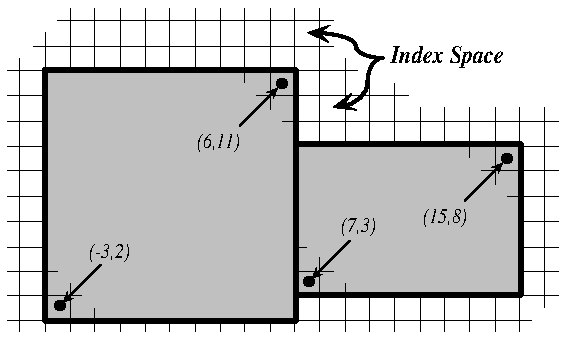
\includegraphics[width=.5\textwidth]{figStructGridBoxes}
\caption{%
A box is a collection of abstract cell-centered indices, described by its
minimum and maximum indices.  Here, two boxes are illustrated.}
\label{fig-struct-boxes}
\end{figure}
The integers may have any value, negative or positive.  The global indexes
allow \hypre{} to discern how data is related spatially, and how it is
distributed across the parallel machine.  The basic component of the grid is a
{\em box}: a collection of abstract cell-centered indices in index space,
described by its ``lower'' and ``upper'' corner indices.  The scalar grid data
is always associated with cell centers, unlike the more general \code{SStruct}
interface which allows data to be associated with box indices in several
different ways.

Each process describes that portion of the grid that it ``owns'', one box at a
time.  For example, the global grid in Figure~\ref{fig-struct-example} can be
described in terms of three boxes, two owned by process 0, and one owned by
process 1.  Figure~\ref{fig-struct-grid} shows the code for setting up the grid
on process 0 (the code for process 1 is similar).
\begin{figure}
\centering
\begin{tabular}{@{}c@{}}
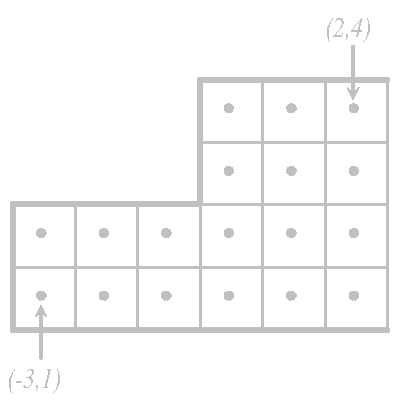
\includegraphics[width=.22\textwidth]{figStructGrid1}\vspace{-.5em} \\ 1
\end{tabular}
\hfill
\begin{tabular}{@{}c@{}}
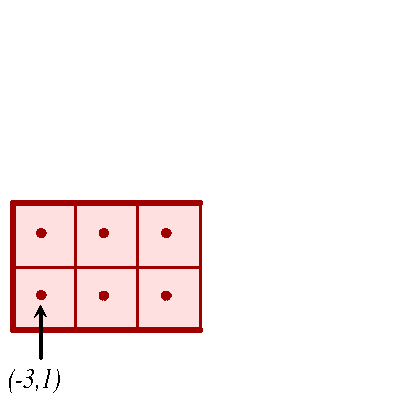
\includegraphics[width=.22\textwidth]{figStructGrid2}\vspace{-.5em} \\ 2
\end{tabular}
\hfill
\begin{tabular}{@{}c@{}}
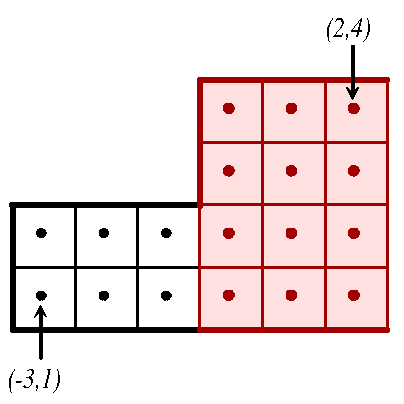
\includegraphics[width=.22\textwidth]{figStructGrid3}\vspace{-.5em} \\ 3
\end{tabular}
\hfill
\begin{tabular}{@{}c@{}}
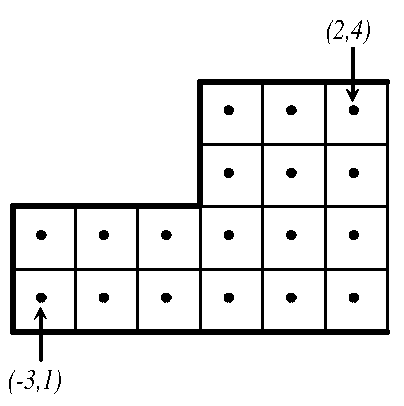
\includegraphics[width=.22\textwidth]{figStructGrid4}\vspace{-.5em} \\ 4
\end{tabular}
\vspace{2em} \\
\begin{minipage}{0.7\textwidth}
\begin{verbatim}
   
    HYPRE_StructGrid grid;
    int ndim        = 2;
    int ilower[][2] = {{-3,1}, {0,1}};
    int iupper[][2] = {{-1,2}, {2,4}};
   
    /* Create the grid object */
1:  HYPRE_StructGridCreate(MPI_COMM_WORLD, ndim, &grid);
    
    /* Set grid extents for the first box */
2:  HYPRE_StructGridSetExtents(grid, ilower[0], iupper[0]);
    
    /* Set grid extents for the second box */
3:  HYPRE_StructGridSetExtents(grid, ilower[1], iupper[1]);
    
    /* Assemble the grid */
4:  HYPRE_StructGridAssemble(grid);
    
\end{verbatim}
\end{minipage}
\caption{%
Code on process 0 for setting up the grid in Figure~\ref{fig-struct-example}.}
\label{fig-struct-grid}
\end{figure}
The ``icons'' at the top of the figure illustrate the result of the numbered
lines of code.  The \code{Create()} routine creates an empty 2D grid object
that lives on the \code{MPI_COMM_WORLD} communicator.  The \code{SetExtents()}
routine adds a new box to the grid.  The \code{Assemble()} routine is a
collective call (i.e., must be called on all processes from a common
synchronization point), and finalizes the grid assembly, making the grid
``ready to use''.

%-----------------------------------------------------------------------------

\section{Setting Up the Struct Stencil}
\label{sec-Struct-Stencil}

The geometry of the discretization stencil is described by an array of indexes,
each representing a relative offset from any given gridpoint on the grid.  For
example, the geometry of the 5-pt stencil for the example problem being
considered can be represented by the list of index offsets shown in
Figure~\ref{fig-struct-stencil-a}.
\begin{figure}
\centering
\mbox{}\hfill
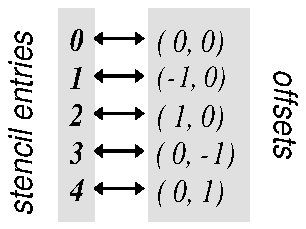
\includegraphics[width=.3\textwidth]{figStructStenc0}
\hfill
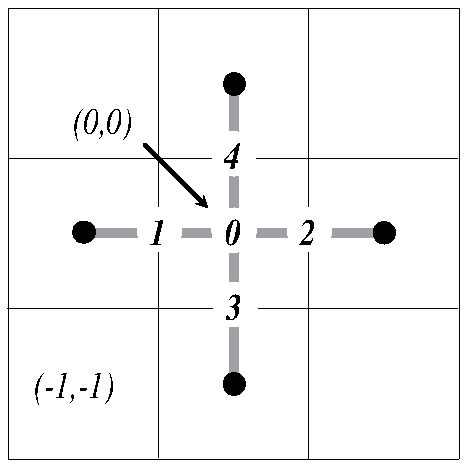
\includegraphics[width=.25\textwidth]{figStructStenc7}
\hfill\mbox{}
\caption{%
Representation of the 5-point discretization stencil for the example problem.}
\label{fig-struct-stencil-a}
\end{figure}
Here, the $(0,0)$ entry represents the ``center'' coefficient, and is the 0th
stencil entry.  The $(0,-1)$ entry represents the ``south'' coefficient, and is
the 3rd stencil entry.  And so on.

On process 0 or 1, the code in Figure~\ref{fig-struct-stencil-b} will set up
the stencil in Figure~\ref{fig-struct-stencil-a}.  The stencil must be the same
on all processes.
\begin{figure}
\centering
\mbox{}\hfill
\begin{tabular}{@{}c@{}}
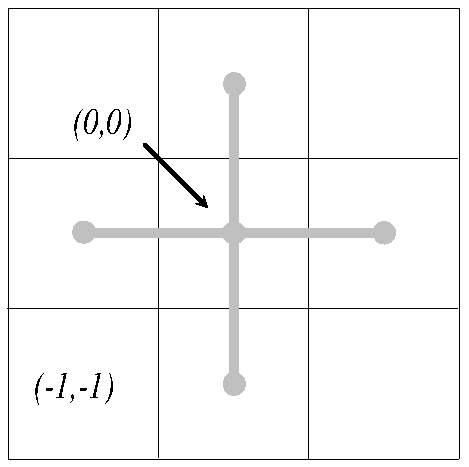
\includegraphics[width=.22\textwidth]{figStructStenc1} \\ 1
\end{tabular}
\hfill
\begin{tabular}{@{}c@{}}
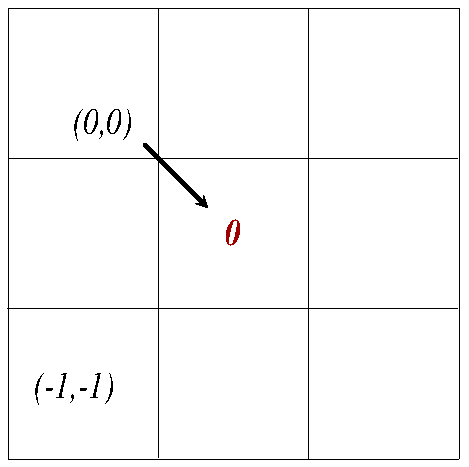
\includegraphics[width=.22\textwidth]{figStructStenc2} \\ 2
\end{tabular}
\hfill
\begin{tabular}{@{}c@{}}
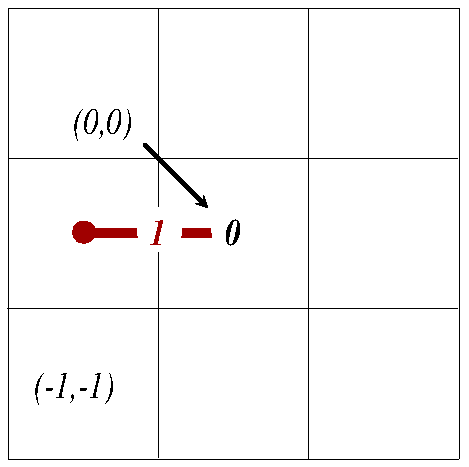
\includegraphics[width=.22\textwidth]{figStructStenc3} \\ 3
\end{tabular}
\hfill\mbox{}
\vspace{1em} \\
\mbox{}\hfill
\begin{tabular}{@{}c@{}}
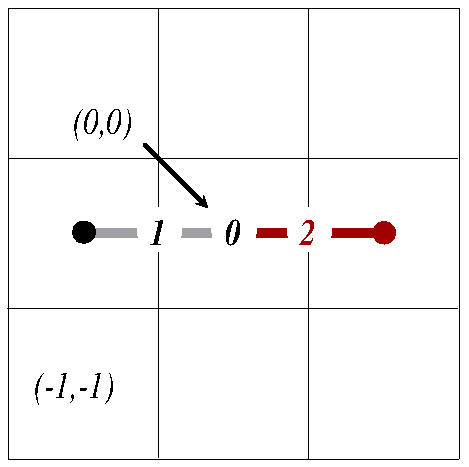
\includegraphics[width=.22\textwidth]{figStructStenc4} \\ 4
\end{tabular}
\hfill
\begin{tabular}{@{}c@{}}
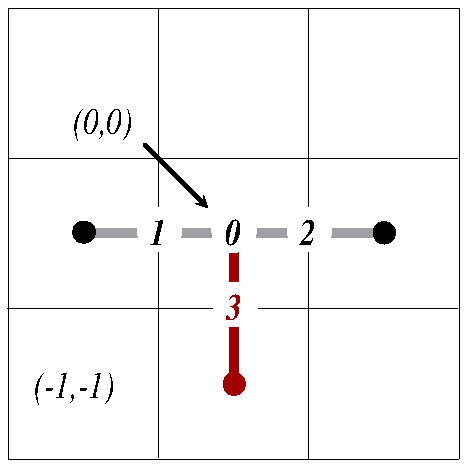
\includegraphics[width=.22\textwidth]{figStructStenc5} \\ 5
\end{tabular}
\hfill
\begin{tabular}{@{}c@{}}
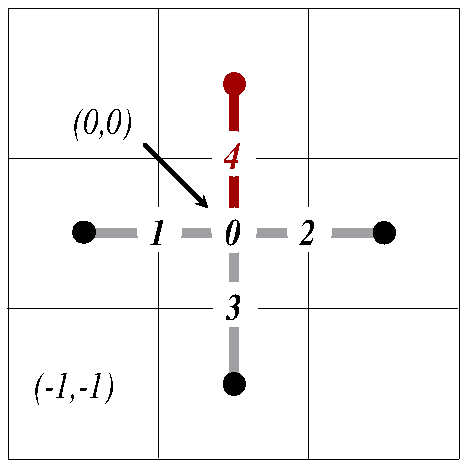
\includegraphics[width=.22\textwidth]{figStructStenc6} \\ 6
\end{tabular}
\hfill\mbox{}
\vspace{2em} \\
\begin{minipage}{0.85\textwidth}
\begin{verbatim}
      
      HYPRE_StructStencil stencil;
      int ndim         = 2;
      int size         = 5;
      int entry;
      int offsets[][2] = {{0,0}, {-1,0}, {1,0}, {0,-1}, {0,1}};
      
      /* Create the stencil object */
  1:  HYPRE_StructStencilCreate(ndim, size, &stencil);
      
      /* Set stencil entries */
      for (entry = 0; entry < size; entry++)
      {
2-6:     HYPRE_StructStencilSetElement(stencil, entry, offsets[entry]);
      }
      
      /* Thats it!  There is no assemble routine */
      
\end{verbatim}
\end{minipage}
\caption{%
Code for setting up the stencil in Figure~\ref{fig-struct-stencil-a}.}
\label{fig-struct-stencil-b}
\end{figure}
The \code{Create()} routine creates an empty 2D, 5-pt stencil object.  The
\code{SetElement()} routine defines the geometry of the stencil and assigns the
stencil numbers for each of the stencil entries.  None of the calls are
collective calls.

%-----------------------------------------------------------------------------

\section{Setting Up the Struct Matrix}
\label{sec-Struct-Matrix}

The matrix is set up in terms of the grid and stencil objects described in
Sections \ref{sec-Struct-Grid} and \ref{sec-Struct-Stencil}.  The coefficients
associated with each stencil entry will typically vary from gridpoint to
gridpoint, but in the example problem being considered, they are as follows
over the entire grid (except at boundaries; see below):
\begin{equation}\label{eqn-stencil-laplacian}
\left [
\begin{array}{ccc}
    & -1 &    \\
 -1 &  4 & -1 \\
    & -1 &    
\end{array}
\right ] .
\end{equation}

On process 0, the code in Figure~\ref{fig-struct-matrix} will set up matrix
values associated with the center (entry 0) and south (entry 3) stencil entries
as given by \ref{eqn-stencil-laplacian} and Figure~\ref{fig-struct-matrix}
(boundaries are ignored here temporarily).
\begin{figure}
\centering
\begin{minipage}{0.75\textwidth}
\begin{verbatim}

HYPRE_StructMatrix  A;
double              values[36];
int                 stencil_indices[2] = {0,3};
int                 i;

HYPRE_StructMatrixCreate(MPI_COMM_WORLD, grid, stencil, &A);
HYPRE_StructMatrixInitialize(A);

for (i = 0; i < 36; i += 2)
{
   values[i]   =  4.0;
   values[i+1] = -1.0;
}

HYPRE_StructMatrixSetBoxValues(A, ilower[0], iupper[0], 2,
                               stencil_indices, values);
HYPRE_StructMatrixSetBoxValues(A, ilower[1], iupper[1], 2,
                               stencil_indices, values);

/* set boundary conditions */
...

HYPRE_StructMatrixAssemble(A);

\end{verbatim}
\end{minipage}
\caption{%
Code for setting up matrix values associated with stencil entries 0 and 3 as
given by \ref{eqn-stencil-laplacian} and Figure~\ref{fig-struct-stencil-a}.}
\label{fig-struct-matrix}
\end{figure}
The \code{Create()} routine creates an empty matrix object.  The
\code{Initialize()} routine indicates that the matrix coefficients (or values)
are ready to be set.  This routine may or may not involve the allocation of
memory for the coefficient data, depending on the implementation.  The optional
\code{Set} routines mentioned later in this chapter and in the Reference
Manual, should be called before this step.  The \code{SetBoxValues()} routine
sets the matrix coefficients for some set of stencil entries over the
gridpoints in some box.  Note that the box need not correspond to any of the
boxes used to create the grid, but values should be set for all gridpoints that
this process ``owns''.  The \code{Assemble()} routine is a collective call, and
finalizes the matrix assembly, making the matrix ``ready to use''.

Matrix coefficients that reach outside of the boundary should be set to zero.
For efficiency reasons, \hypre{} does not do this automatically.  The most
natural time to insure this is when the boundary conditions are being set, and
this is most naturally done after the coefficients on the grid's interior have
been set.  For example, during the implementation of the Dirichlet boundary
condition on the lower boundary of the grid in Figure~\ref{fig-struct-example},
the ``south'' coefficient must be set to zero.  To do this on process 0, the
code in Figure~\ref{fig-struct-matrix-boundary} could be used:
\begin{figure}
\centering
\begin{minipage}{0.8\textwidth}
\begin{verbatim}

int  ilower[2] = {-3, 1};
int  iupper[2] = { 2, 1};

/* create matrix and set interior coefficients */
...

/* implement boundary conditions */
...

for (i = 0; i < 12; i++)
{
   values[i] =  0.0;
}

i = 3;
HYPRE_StructMatrixSetBoxValues(A, ilower, iupper, 1, &i, values);

/* complete implementation of boundary conditions */
...

\end{verbatim}
\end{minipage}
\caption{%
Code for adjusting boundary conditions along the lower grid boundary in
Figure~\ref{fig-struct-example}.}
\label{fig-struct-matrix-boundary}
\end{figure}

%-----------------------------------------------------------------------------

\section{Setting Up the Struct Right-Hand-Side Vector}
\label{sec-Struct-RHS}

The right-hand-side vector is set up similarly to the matrix set up described
in Section \ref{sec-Struct-Matrix} above.  The main difference is that there is
no stencil (note that a stencil currently does appear in the interface, but
this will eventually be removed).

On process 0, the code in Figure~\ref{fig-struct-rhs} will set up the
right-hand-side vector values.
\begin{figure}
\centering
\begin{minipage}{0.8\textwidth}
\begin{verbatim}

HYPRE_StructVector  b;
double              values[18];
int                 i;

HYPRE_StructVectorCreate(MPI_COMM_WORLD, grid, &b);
HYPRE_StructVectorInitialize(b);

for (i = 0; i < 18; i++)
{
   values[i]   =  0.0;
}

HYPRE_StructVectorSetBoxValues(b, ilower[0], iupper[0], values);
HYPRE_StructVectorSetBoxValues(b, ilower[1], iupper[1], values);

HYPRE_StructVectorAssemble(b);

\end{verbatim}
\end{minipage}
\caption{%
Code for setting up right-hand-side vector values.}
\label{fig-struct-rhs}
\end{figure}
The \code{Create()} routine creates an empty vector object.  The
\code{Initialize()} routine indicates that the vector coefficients (or values)
are ready to be set.  This routine follows the same rules as its corresponding
\code{Matrix} routine.  The \code{SetBoxValues()} routine sets the vector
coefficients over the gridpoints in some box, and again, follows the same rules
as its corresponding \code{Matrix} routine.  The \code{Assemble()} routine is a
collective call, and finalizes the vector assembly, making the vector ``ready
to use''.

%-----------------------------------------------------------------------------

\section{Symmetric Matrices}
\label{sec-Symmetric-Matrices}

Some solvers and matrix storage schemes provide capabilities for significantly
reducing memory usage when the coefficient matrix is symmetric.  In this
situation, each off-diagonal coefficient appears twice in the matrix, but only
one copy needs to be stored.  The \code{Struct} interface provides support for
matrix and solver implementations that use symmetric storage via the
\code{SetSymmetric()} routine.

To describe this in more detail, consider again the 5-pt finite-volume
discretization of (\ref{eqn-laplacian}) on the grid pictured in
Figure~\ref{fig-struct-example}.  Because the discretization is symmetric, only
half of the off-diagonal coefficients need to be stored.  To turn symmetric
storage on, the following line of code needs to be inserted somewhere between
the \code{Create()} and \code{Initialize()} calls.
\begin{display}
\begin{verbatim}

HYPRE_StructMatrixSetSymmetric(A, 1);

\end{verbatim}
\end{display}
The coefficients for the entire stencil can be passed in as before.  Note that
symmetric storage may or may not actually be used, depending on the underlying
storage scheme.  Currently in \hypre{}, the \code{Struct} interface always uses
symmetric storage.

To most efficiently utilize the \code{Struct} interface for symmetric matrices,
notice that only half of the off-diagonal coefficients need to be set.  To do
this for the example being considered, we simply need to redefine the 5-pt
stencil of Section \ref{sec-Struct-Stencil} to an ``appropriate'' 3-pt stencil,
then set matrix coefficients (as in Section \ref{sec-Struct-Matrix}) for these
three stencil elements {\em only}.  For example, we could use the following
stencil
\begin{equation}\label{eqn-symmetric-stencil}
\left [
\begin{array}{ccc}
~~~~~~ & ( 0, 1) &         \\
~~~~~~ & ( 0, 0) & ( 1, 0) \\
~~~~~~ &         &        
\end{array}
\right ] .
\end{equation}
This 3-pt stencil provides enough information to recover the full 5-pt stencil
geometry and associated matrix coefficients.

%=============================================================================
%=============================================================================

\chapter{Semi-Structured-Grid System Interface (SStruct)}
\label{ch-SStruct}

The \code{SStruct} interface is appropriate for applications with grids that
are mostly---but not entirely---structured, e.g. block-structured grids (see
Figure~\ref{fig-sstruct-example}), composite grids in structured adaptive mesh
refinement (AMR) applications (see Figure~\ref{fig-sstruct-samr-grid}), and
overset grids.  In addition, it supports more general PDEs than the
\code{Struct} interface by allowing multiple variables (system PDEs) and
multiple variable types (e.g. cell-centered, face-centered, etc.).  The
interface provides access to data structures and linear solvers in \hypre{}
that are designed for semi-structured grid problems, but also to the most
general data structures and solvers.
%These latter solvers are usually provided via the \code{FEI} or \code{IJ}
%interfaces described in Chapters~\ref{ch-FEI} and \ref{ch-IJ}.

The \code{SStruct} grid is composed out of a number of structured grid {\em
parts}, where the physical inter-relationship between the parts is arbitrary.
Each part is constructed out of two basic components: boxes (see
Figure~\ref{fig-struct-boxes}) and {\em variables}.  Variables represent the
actual unknown quantities in the grid, and are associated with the box indices
in a variety of ways, depending on their types.  In \hypre{}, variables may be
cell-centered, node-centered, face-centered, or edge-centered.  Face-centered
variables are split into x-face, y-face, and z-face, and edge-centered
variables are split into x-edge, y-edge, and z-edge.  See Figure
\ref{fig-gridvars} for an illustration in 2D.

\begin{figure}
\centering
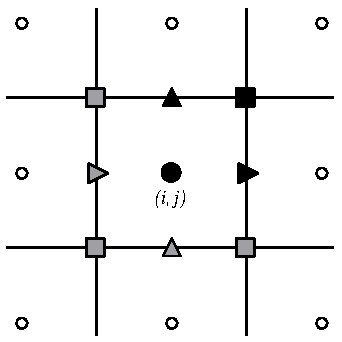
\includegraphics[width=.3\textwidth]{figSStructGridVars}
\caption{%
Grid variables in \hypre{} are referenced by the abstract cell-centered index
to the left and down in 2D (analogously in 3D).  In the figure, index $(i,j)$
is used to reference the variables in black.  The variables in grey---although
contained in the pictured cell---are not referenced by the $(i,j)$ index.}
\label{fig-gridvars}
\end{figure}

The \code{SStruct} interface uses a {\em graph} to allow nearly arbitrary
relationships between part data.  The graph is constructed from stencils or
finite element stiffness matrices plus some additional data-coupling information
set by the \code{GraphAddEntries()} routine.  Two other methods for relating
part data are the \code{GridSetNeighborPart()} and \code{GridSetSharedPart()}
routines, which are particularly well suited for block-structured grid problems.
The latter is useful for finite element codes.

There are five basic steps involved in setting up the linear system to be
solved:
%\begin{enumerate}
\begin{list}{\arabic{enumi}.}{\usecounter{enumi}\setlength{\itemsep}{0in}}
\item set up the grid,
\item set up the stencils (if needed),
\item set up the graph,
\item set up the matrix,
\item set up the right-hand-side vector.
\end{list}
%\end{enumerate}
%In the remainder of this section, we consider three examples: block-structured
%grid problems with stencils (Section~\ref{sec-Block-Structured-Grids});
%block-structured grid problems with finite elements
%(Section~\ref{sec-Block-Structured-Grids-FEM}); and structured adaptive mesh
%refinement problems (Section~\ref{sec-Structured-Adaptive-Mesh-Refinement}).

%-----------------------------------------------------------------------------

\section{Block-Structured Grids with Stencils}
\label{sec-Block-Structured-Grids}

In this section, we describe how to use the \code{SStruct} interface to define
block-structured grid problems.  We do this primarily by example, paying
particular attention to the construction of stencils and the use of the
\code{GridSetNeighborPart()} interface routine.

Consider the solution of the diffusion equation
\begin{equation} \label{eqn-block-diffusion}
- \nabla \cdot (D \nabla u) + \sigma u = f
\end{equation}
on the block-structured grid in Figure~\ref{fig-sstruct-example}, where $D$ is
a scalar diffusion coefficient, and $\sigma \geq 0$.  The discretization
\cite{JEMorel_RMRoberts_MJShashkov_1998} introduces three different types of
variables: cell-centered, $x$-face, and $y$-face.  The three discretization
stencils that couple these variables are also given in the figure.  The
information in this figure is essentially all that is needed to describe the
nonzero structure of the linear system we wish to solve.

\begin{figure}
\centering
\mbox{}\hfill
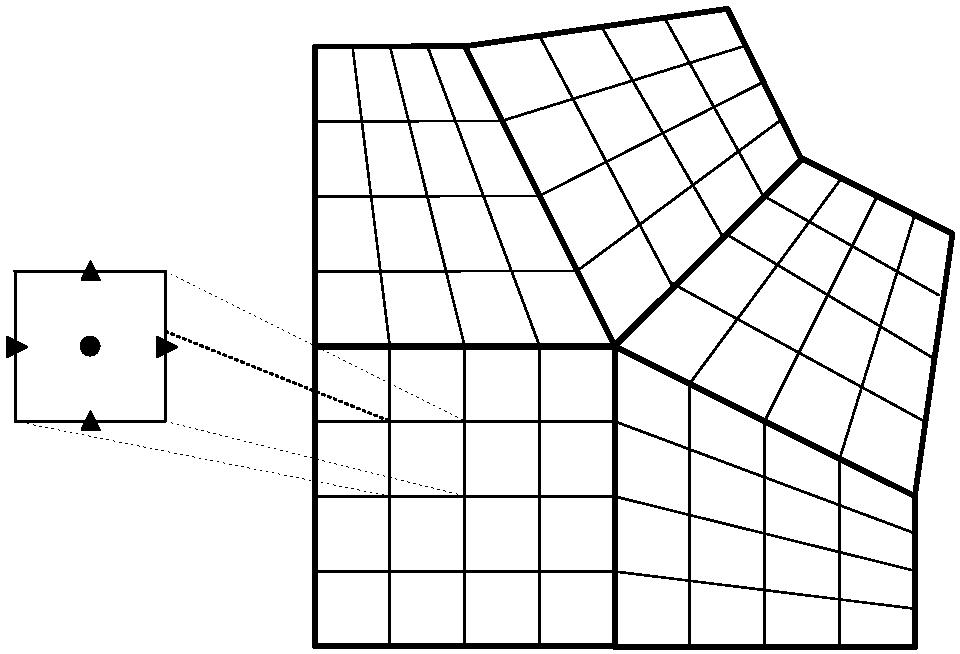
\includegraphics[width=.45\textwidth]{figSStructExample1a}
\hfill
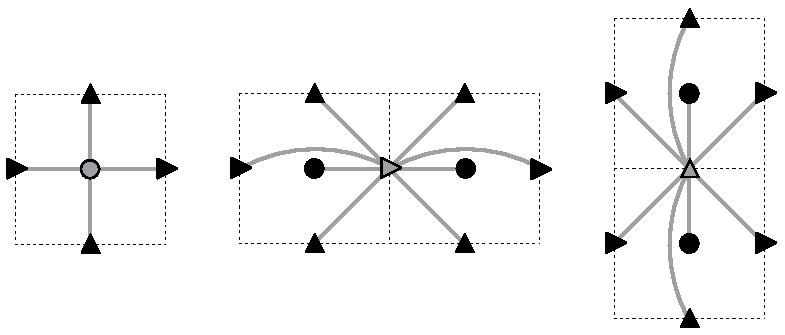
\includegraphics[width=.4\textwidth]{figSStructExample1b}
\hfill\mbox{}
\caption{%
Example of a block-structured grid with five logically-rectangular blocks and
three variables types: cell-centered, $x$-face, and $y$-face.  Discretization
stencils for the cell-centered (left), $x$-face (middle), and $y$-face (right)
variables are also pictured.}
\label{fig-sstruct-example}

\end{figure}
\begin{figure}
\centering
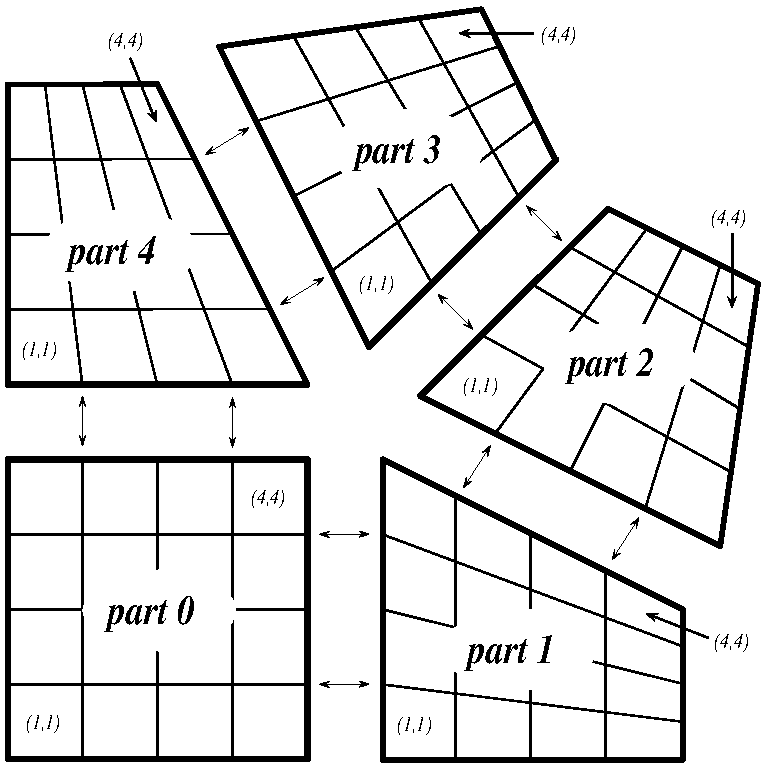
\includegraphics[width=.6\textwidth]{figSStructExample1c}
\caption{%
One possible labeling of the grid in Figure~\ref{fig-sstruct-example}.}
\label{fig-sstruct-example-parts}
\end{figure}

The grid in Figure~\ref{fig-sstruct-example} is defined in terms of five
separate logically-rectangular parts as shown in
Figure~\ref{fig-sstruct-example-parts}, and each part is given a unique label
between 0 and 4.  Each part consists of a single box with lower index $(1,1)$
and upper index $(4,4)$ (see Section~\ref{sec-Struct-Grid}), and the grid data
is distributed on five processes such that data associated with part~$p$ lives
on process~$p$.  Note that in general, parts may be composed out of arbitrary
unions of boxes, and indices may consist of non-positive integers (see
Figure~\ref{fig-struct-boxes}).  Also note that the \code{SStruct} interface
expects a domain-based data distribution by boxes, but the actual distribution
is determined by the user and simply described (in parallel) through the
interface.

\begin{figure}
\centering
\begin{tabular}{@{}c@{}}
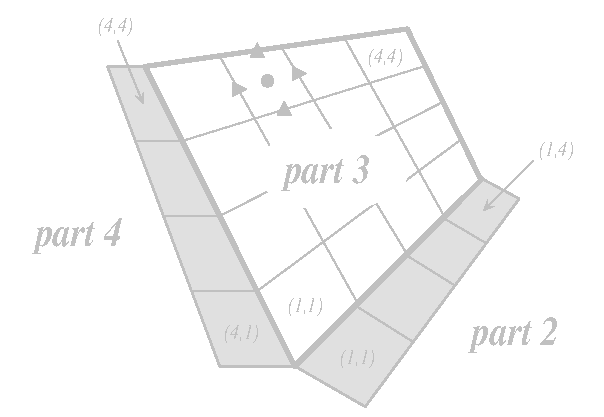
\includegraphics[width=.28\textwidth]{figSStructGrid1} \\ 1
\end{tabular}
\hfill
\begin{tabular}{@{}c@{}}
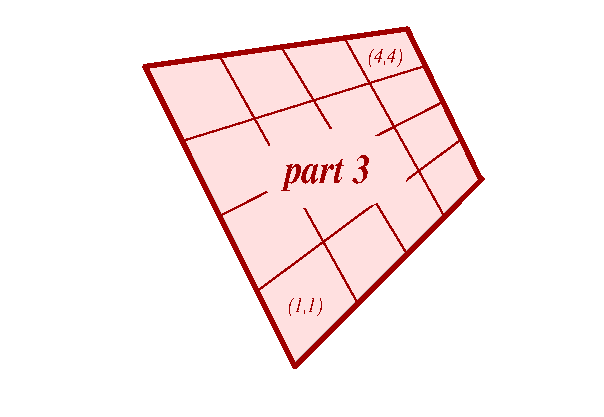
\includegraphics[width=.28\textwidth]{figSStructGrid2} \\ 2
\end{tabular}
\hfill
\begin{tabular}{@{}c@{}}
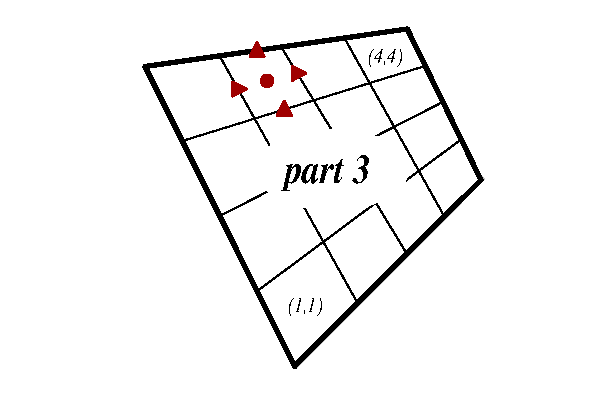
\includegraphics[width=.28\textwidth]{figSStructGrid3} \\ 3
\end{tabular}
\vspace{1em} \\
\begin{tabular}{@{}c@{}}
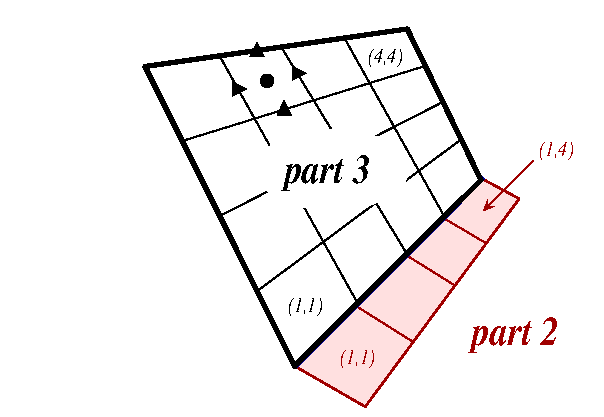
\includegraphics[width=.28\textwidth]{figSStructGrid4} \\ 4
\end{tabular}
\hfill
\begin{tabular}{@{}c@{}}
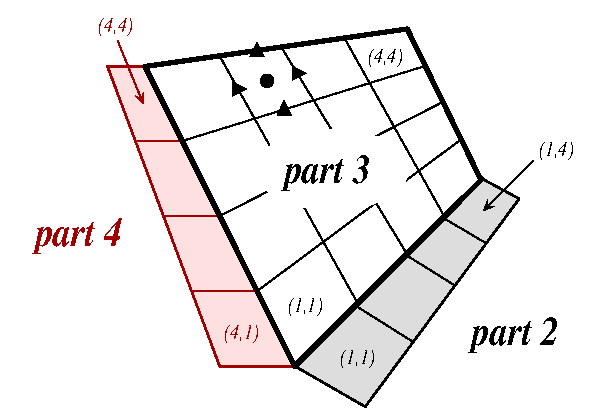
\includegraphics[width=.28\textwidth]{figSStructGrid5} \\ 5
\end{tabular}
\hfill
\begin{tabular}{@{}c@{}}
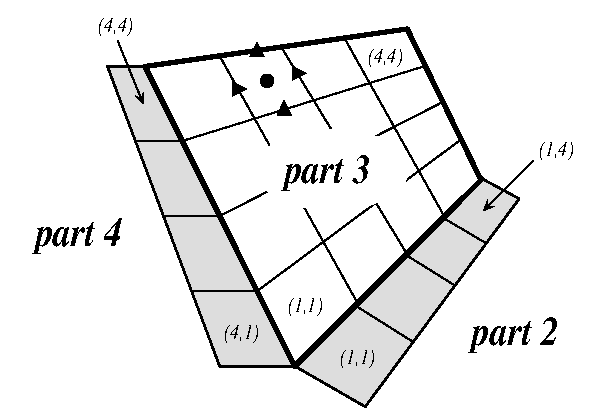
\includegraphics[width=.28\textwidth]{figSStructGrid6} \\ 6
\end{tabular}
\vspace{2em} \\
\begin{minipage}{0.9\textwidth}
\begin{verbatim}
    
    HYPRE_SStructGrid grid;
    int ndim = 2, nparts = 5, nvars = 3, part = 3;
    int extents[][2] = {{1,1}, {4,4}};
    int vartypes[]   = {HYPRE_SSTRUCT_VARIABLE_CELL,
                        HYPRE_SSTRUCT_VARIABLE_XFACE,
                        HYPRE_SSTRUCT_VARIABLE_YFACE};
    int nb2_n_part      = 2,              nb4_n_part      = 4;
    int nb2_exts[][2]   = {{1,0}, {4,0}}, nb4_exts[][2]   = {{0,1}, {0,4}};
    int nb2_n_exts[][2] = {{1,1}, {1,4}}, nb4_n_exts[][2] = {{4,1}, {4,4}};
    int nb2_map[2]      = {1,0},          nb4_map[2]      = {0,1};
    int nb2_dir[2]      = {1,-1},         nb4_dir[2]      = {1,1};

1:  HYPRE_SStructGridCreate(MPI_COMM_WORLD, ndim, nparts, &grid);
    
    /* Set grid extents and grid variables for part 3 */
2:  HYPRE_SStructGridSetExtents(grid, part, extents[0], extents[1]);
3:  HYPRE_SStructGridSetVariables(grid, part, nvars, vartypes);
    
    /* Set spatial relationship between parts 3 and 2, then parts 3 and 4 */
4:  HYPRE_SStructGridSetNeighborPart(grid, part, nb2_exts[0], nb2_exts[1],
       nb2_n_part, nb2_n_exts[0], nb2_n_exts[1], nb2_map, nb2_dir);
5:  HYPRE_SStructGridSetNeighborPart(grid, part, nb4_exts[0], nb4_exts[1],
       nb4_n_part, nb4_n_exts[0], nb4_n_exts[1], nb4_map, nb4_dir);
    
6:  HYPRE_SStructGridAssemble(grid);
    
\end{verbatim}
\end{minipage}
\caption{%
Code on process 3 for setting up the grid in Figure~\ref{fig-sstruct-example}.}
\label{fig-sstruct-grid}
\end{figure}

As with the \code{Struct} interface, each process describes that portion of the
grid that it ``owns'', one box at a time.  Figure~\ref{fig-sstruct-grid} shows
the code for setting up the grid on process~3 (the code for the other processes
is similar).  The ``icons'' at the top of the figure illustrate the result of
the numbered lines of code.  Process~3 needs to describe the data pictured in
the bottom-right of the figure.  That is, it needs to describe part~3 plus some
additional neighbor information that ties part~3 together with the rest of the
grid.  The \code{Create()} routine creates an empty 2D grid object with five
parts that lives on the \code{MPI_COMM_WORLD} communicator.  The
\code{SetExtents()} routine adds a new box to the grid.  The
\code{SetVariables()} routine associates three variables of type cell-centered,
$x$-face, and $y$-face with part~3.

At this stage, the description of the data on part~3 is complete.  However, the
spatial relationship between this data and the data on neighboring parts is not
yet defined.  To do this, we need to relate the index space for part~3 with the
index spaces of parts 2 and~4.  More specifically, we need to tell the interface
that the two grey boxes neighboring part~3 in the bottom-right of
Figure~\ref{fig-sstruct-grid} also correspond to boxes on parts 2 and~4.  This
is done through the two calls to the \code{SetNeighborPart()} routine.  We
discuss only the first call, which describes the grey box on the right of the
figure.  Note that this grey box lives outside of the box extents for the grid
on part~3, but it can still be described using the index-space for part~3
(recall Figure~\ref{fig-struct-boxes}).  That is, the grey box has extents
$(1,0)$ and $(4,0)$ on part~3's index-space, which is outside of part~3's grid.
The arguments for the \code{SetNeighborPart()} call are simply the lower and
upper indices on part~3 and the corresponding indices on part~2.  The final two
arguments to the routine indicate that the positive $x$-direction on part~3
(i.e., the $i$ component of the tuple $(i,j)$) corresponds to the positive
$y$-direction on part~2 and that the positive $y$-direction on part~3
corresponds to the positive $x$-direction on part~2.

The \code{Assemble()} routine is a collective call (i.e., must be called on all
processes from a common synchronization point), and finalizes the grid
assembly, making the grid ``ready to use''.

With the neighbor information, it is now possible to determine where off-part
stencil entries couple.  Take, for example, any shared part boundary such as
the boundary between parts 2 and~3.  Along these boundaries, some stencil
entries reach outside of the part.  If no neighbor information is given, these
entries are effectively zeroed out, i.e., they don't participate in the
discretization.  However, with the additional neighbor information, when a
stencil entry reaches into a neighbor box it is then coupled to the part
described by that neighbor box information.

Another important consequence of the use of the \code{SetNeighborPart()} routine
is that it can declare variables on different parts as being the same.  For
example, the face variables on the boundary of parts 2 and~3 are recognized as
being shared by both parts (prior to the \code{SetNeighborPart()} call, there
were two distinct sets of variables).  Note also that these variables are of
different types on the two parts; on part~2 they are $x$-face variables, but on
part~3 they are $y$-face variables.

For brevity, we consider only the description of the $y$-face stencil in
Figure~\ref{fig-sstruct-example}, i.e. the third stencil in the figure.  To do
this, the stencil entries are assigned unique labels between 0 and 8 and their
``offsets'' are described relative to the ``center'' of the stencil.  This
process is illustrated in Figure \ref{fig-sstruct-stencil}.  Nine calls are
made to the routine \code{HYPRE_SStructStencilSetEntry()}.  As an example, the
call that describes stencil entry 5 in the figure is given the entry number~5,
the offset $(-1,0)$, and the identifier for the $x$-face variable (the variable
to which this entry couples).  Recall from Figure~\ref{fig-gridvars} the
convention used for referencing variables of different types.  The geometry
description uses the same convention, but with indices numbered relative to the
referencing index $(0,0)$ for the stencil's center.
Figure~\ref{fig-sstruct-graph} shows the code for setting up the graph .

\begin{figure}
\centering
\mbox{}\hfill
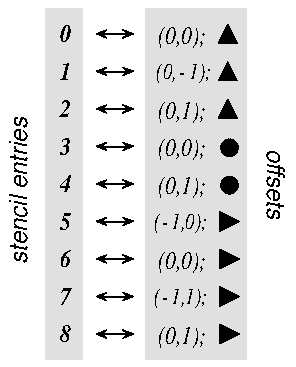
\includegraphics[width=.25\textwidth]{figSStructStenc0}
\hfill
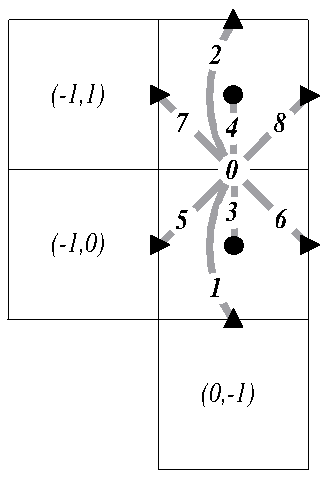
\includegraphics[width=.2\textwidth]{figSStructStenc1}
\hfill\mbox{}
\caption{%
Assignment of labels and geometries to the $y$-face stencil in
Figure~\ref{fig-sstruct-example}.}
\label{fig-sstruct-stencil}
\end{figure}

\begin{figure}
\centering
\begin{tabular}{@{}c@{}}
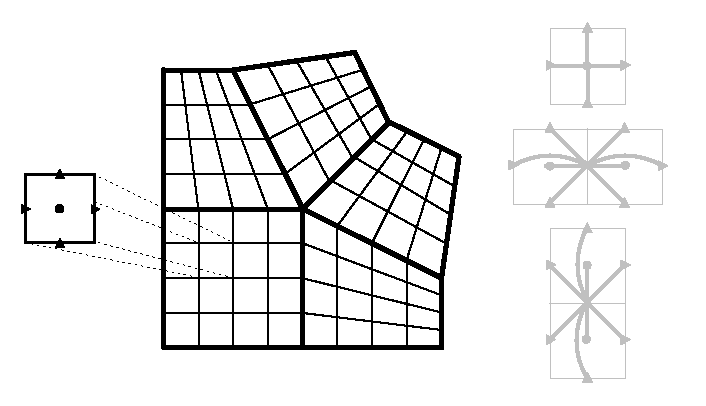
\includegraphics[width=.32\textwidth]{figSStructGraph1}\vspace{-.5em} \\ 1
\end{tabular}
\hfill
\begin{tabular}{@{}c@{}}
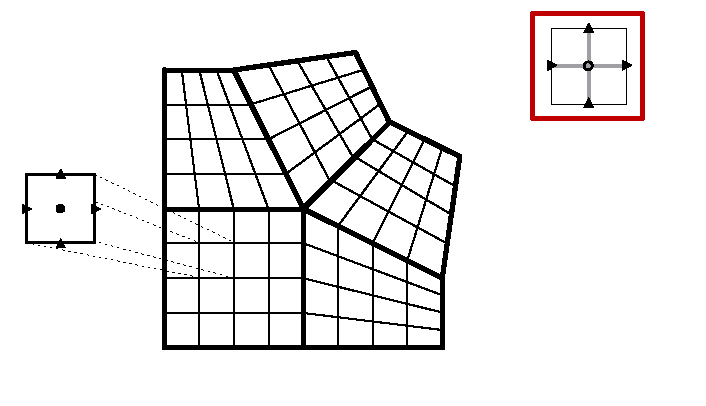
\includegraphics[width=.32\textwidth]{figSStructGraph2}\vspace{-.5em} \\ 2
\end{tabular}
\hfill
\begin{tabular}{@{}c@{}}
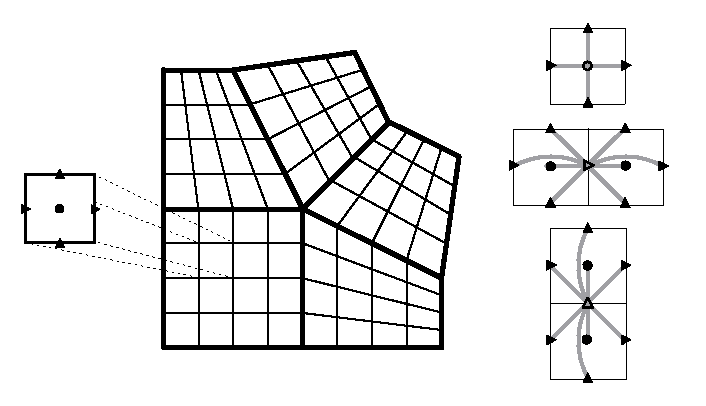
\includegraphics[width=.32\textwidth]{figSStructGraph5}\vspace{-.5em} \\ 3
\end{tabular}
\vspace{1em} \\
\begin{minipage}{0.9\textwidth}
\begin{verbatim}
    
    HYPRE_SStructGraph graph;
    HYPRE_SStructStencil c_stencil, x_stencil, y_stencil;
    int c_var = 0, x_var = 1, y_var = 2;
    int part;
    
1:  HYPRE_SStructGraphCreate(MPI_COMM_WORLD, grid, &graph);
    
    /* Set the cell-centered, x-face, and y-face stencils for each part */
    for (part = 0; part < 5; part++)
    {
2:     HYPRE_SStructGraphSetStencil(graph, part, c_var, c_stencil);
       HYPRE_SStructGraphSetStencil(graph, part, x_var, x_stencil);
       HYPRE_SStructGraphSetStencil(graph, part, y_var, y_stencil);
    }
    
3:  HYPRE_SStructGraphAssemble(graph);

\end{verbatim}
\end{minipage}
\caption{%
Code on process 3 for setting up the graph for Figure~\ref{fig-sstruct-example}.}
\label{fig-sstruct-graph}
\end{figure}

With the above, we now have a complete description of the nonzero structure for
the matrix.  The matrix coefficients are then easily set in a manner similar to
what is described in Section~\ref{sec-Struct-Matrix} using routines
\code{MatrixSetValues()} and \code{MatrixSetBoxValues()} in the \code{SStruct}
interface.  As before, there are also \code{AddTo} variants of these routines.
Likewise, setting up the right-hand-side is similar to what is described in
Section~\ref{sec-Struct-RHS}.  See the \hypre{} reference manual for details.

An alternative approach for describing the above problem through the interface
is to use the \code{GraphAddEntries()} routine instead of the
\code{GridSetNeighborPart()} routine.  In this approach, the five parts would be
explicitly ``sewn'' together by adding non-stencil couplings to the matrix
graph.  The main downside to this approach for block-structured grid problems
is that variables along block boundaries are no longer considered to be the
same variables on the corresponding parts that share these boundaries.  For
example, any face variable along the boundary between parts 2 and~3 in
Figure~\ref{fig-sstruct-example} would represent two different variables that
live on different parts.  To ``sew'' the parts together correctly, we would
need to explicitly select one of these variables as the representative that
participates in the discretization, and make the other variable a dummy
variable that is decoupled from the discretization by zeroing out appropriate
entries in the matrix.  All of these complications are avoided by using the
\code{GridSetNeighborPart()} for this example.

%-----------------------------------------------------------------------------

\section{Block-Structured Grids with Finite Elements}
\label{sec-Block-Structured-Grids-FEM}

In this section, we describe how to use the \code{SStruct} interface to define
block-structured grid problems with finite elements.  We again do this by
example, paying particular attention to the use of the \code{FEM} interface
routines and the \code{GridSetSharedPart()} routine.  See example code
\file{ex14.c} for a complete implementation.

Consider a nodal finite element (FEM) discretization of the Laplace equation on
the star-shaped grid in Figure~\ref{fig-sstruct-fem-example}.  The local FEM
stiffness matrix in the figure describes the coupling between the grid
variables.  Although we could still describe this problem using stencils as in
Section~\ref{sec-Block-Structured-Grids}, an FEM-based approach (available in
\hypre{} version \code{2.6.0b} and later) is a more natural alternative.

\begin{figure} [t]
\centering
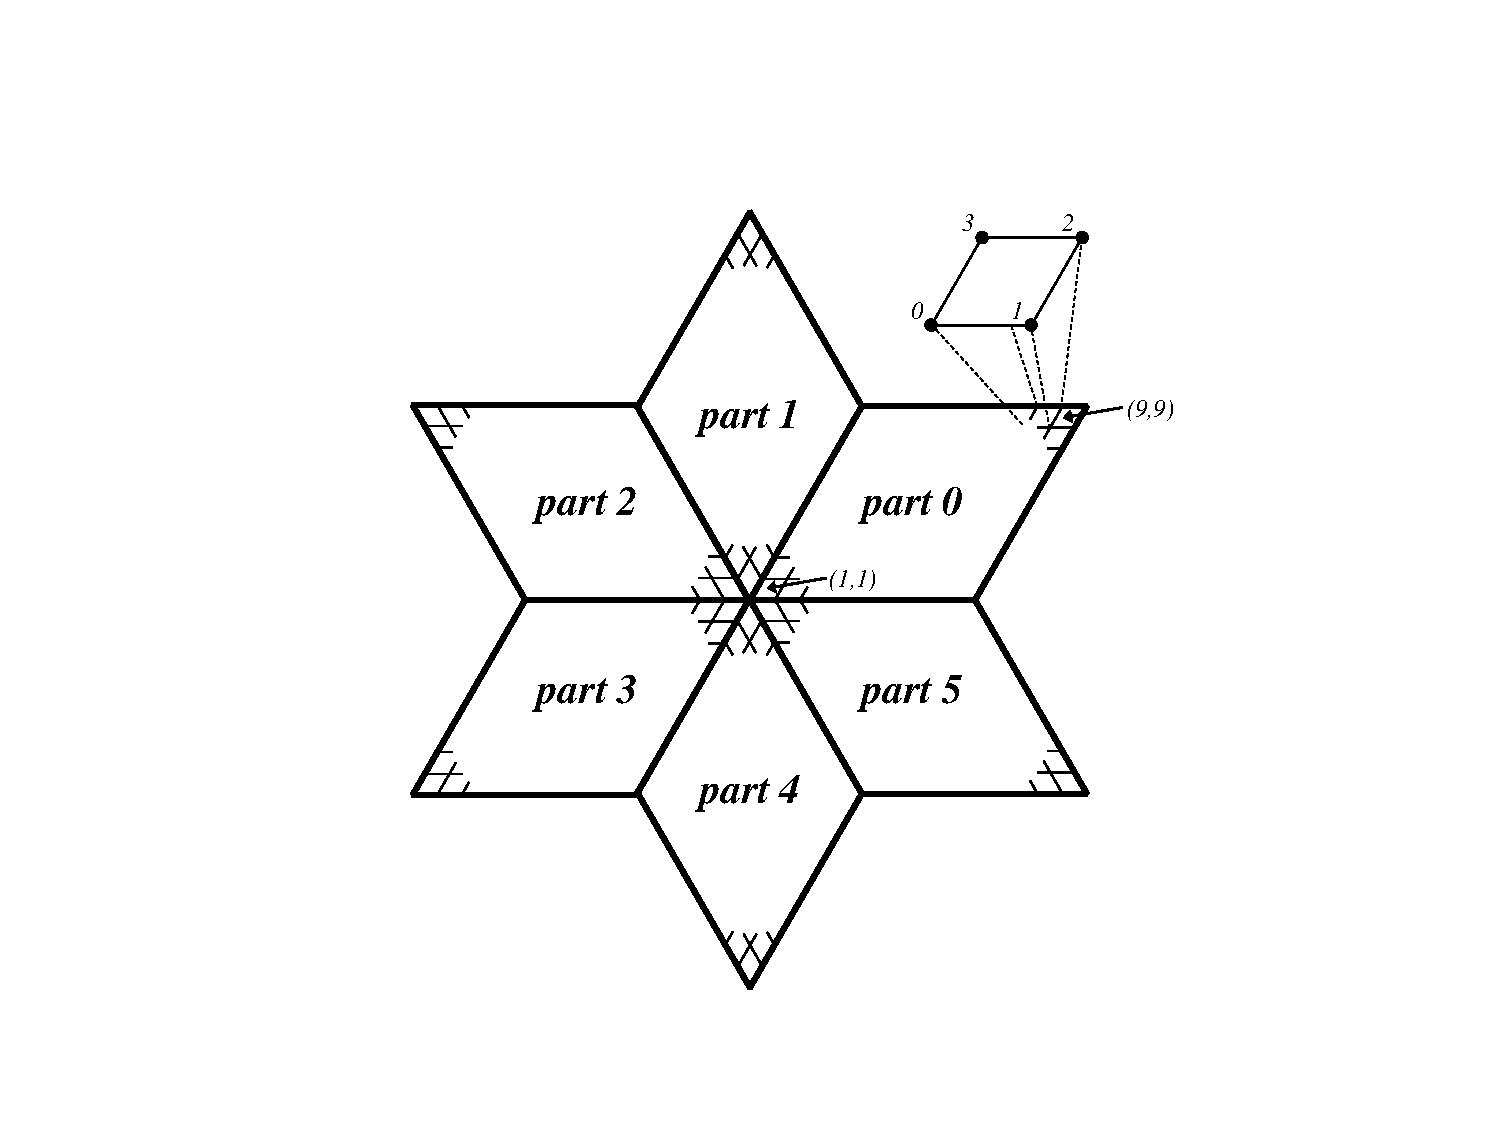
\includegraphics[width=.54\textwidth]{figSStructExample3a}
\hfill
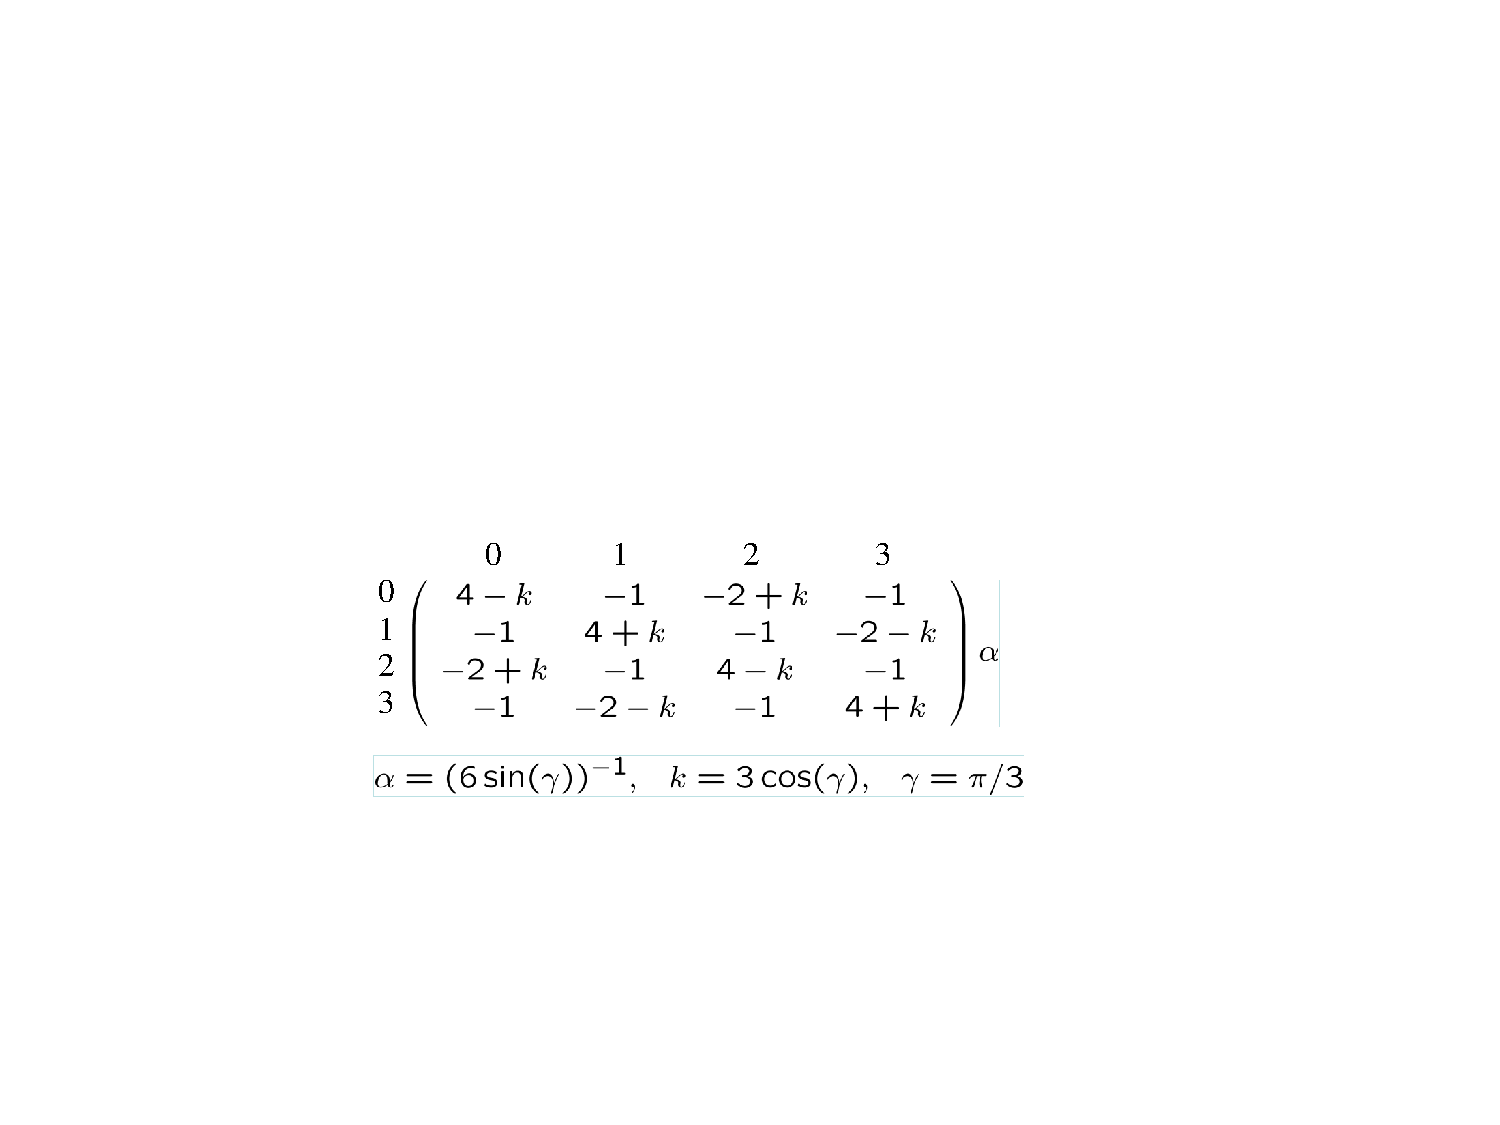
\includegraphics[width=.44\textwidth]{figSStructExample3b}
\caption{%
Example of a star-shaped grid with six logically-rectangular blocks and one
nodal variable.  Each block has an angle at the origin given by $\gamma=\pi/3$.
The finite element stiffness matrix (right) is given in terms of the pictured
variable ordering (left).}
\label{fig-sstruct-fem-example}
\end{figure}

%\begin{figure}
%\centering
%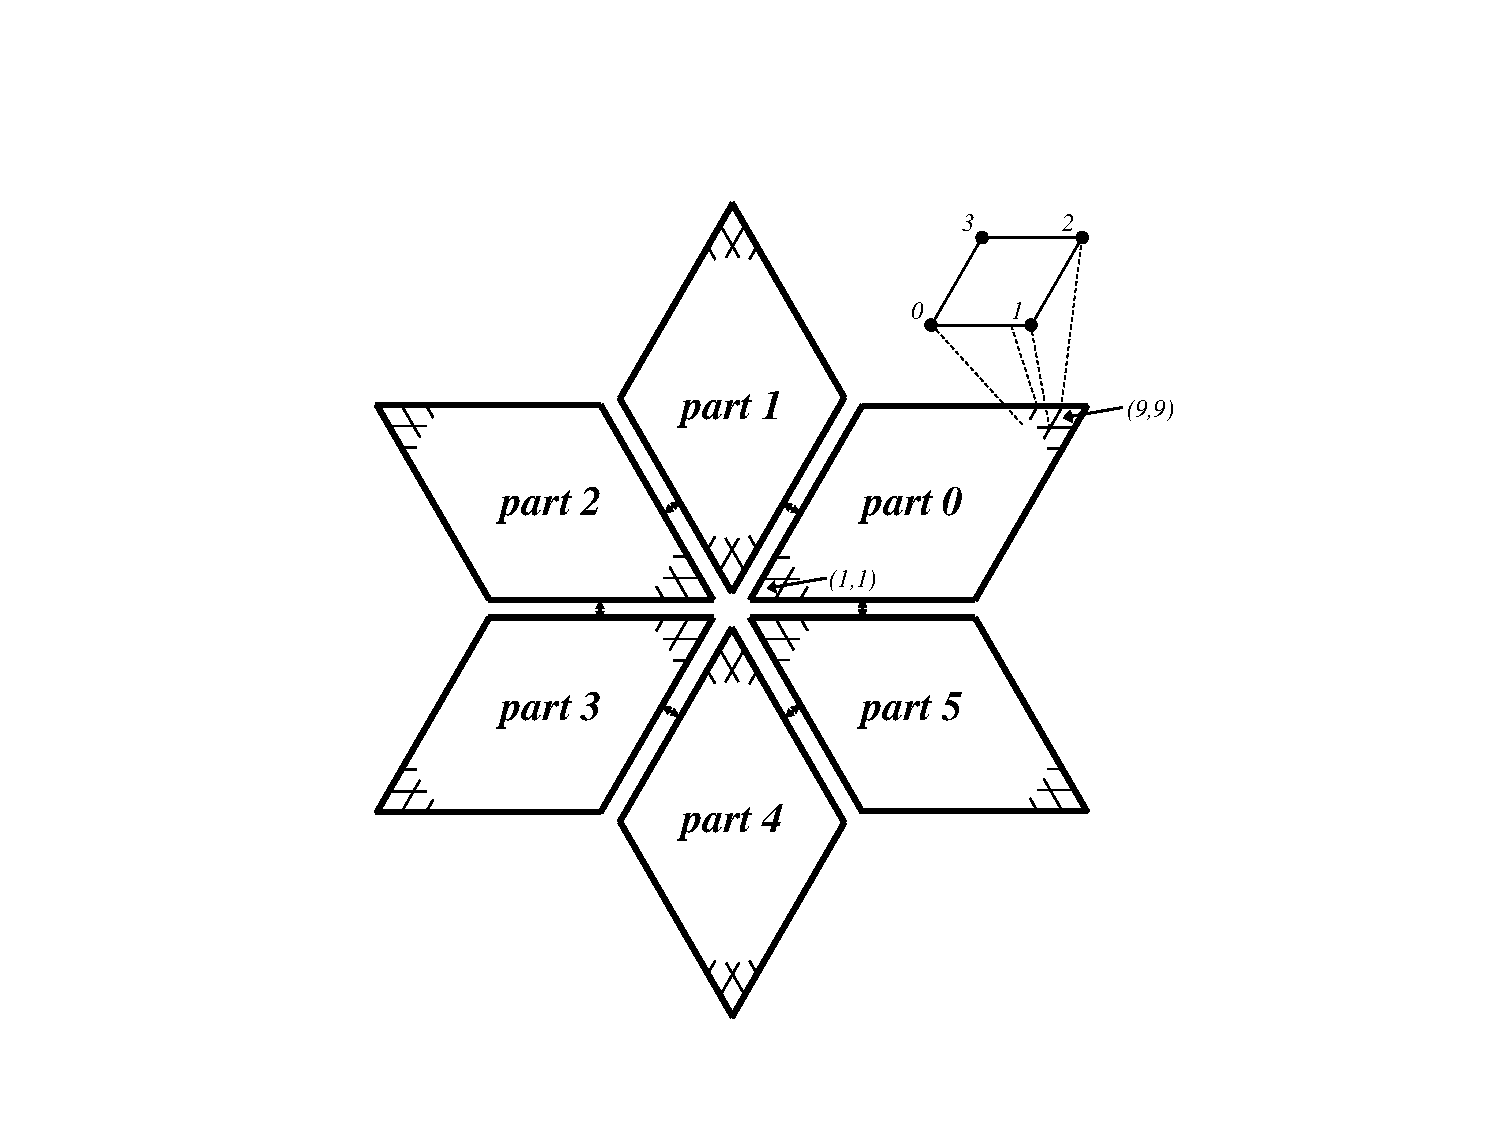
\includegraphics[width=.5\textwidth]{figSStructExample3c}
%\caption{%
%One possible labeling of the grid in Figure~\ref{fig-sstruct-fem-example}.}
%\label{fig-sstruct-fem-example-parts}
%\end{figure}

The grid in Figure~\ref{fig-sstruct-fem-example} is defined in terms of six
separate logically-rectangular parts, and each part is given a unique label
between 0 and 5.  Each part consists of a single box with lower index $(1,1)$
and upper index $(9,9)$, and the grid data is distributed on six processes such
that data associated with part~$p$ lives on process~$p$.

\begin{figure}
\centering
\begin{tabular}{@{}c@{}}
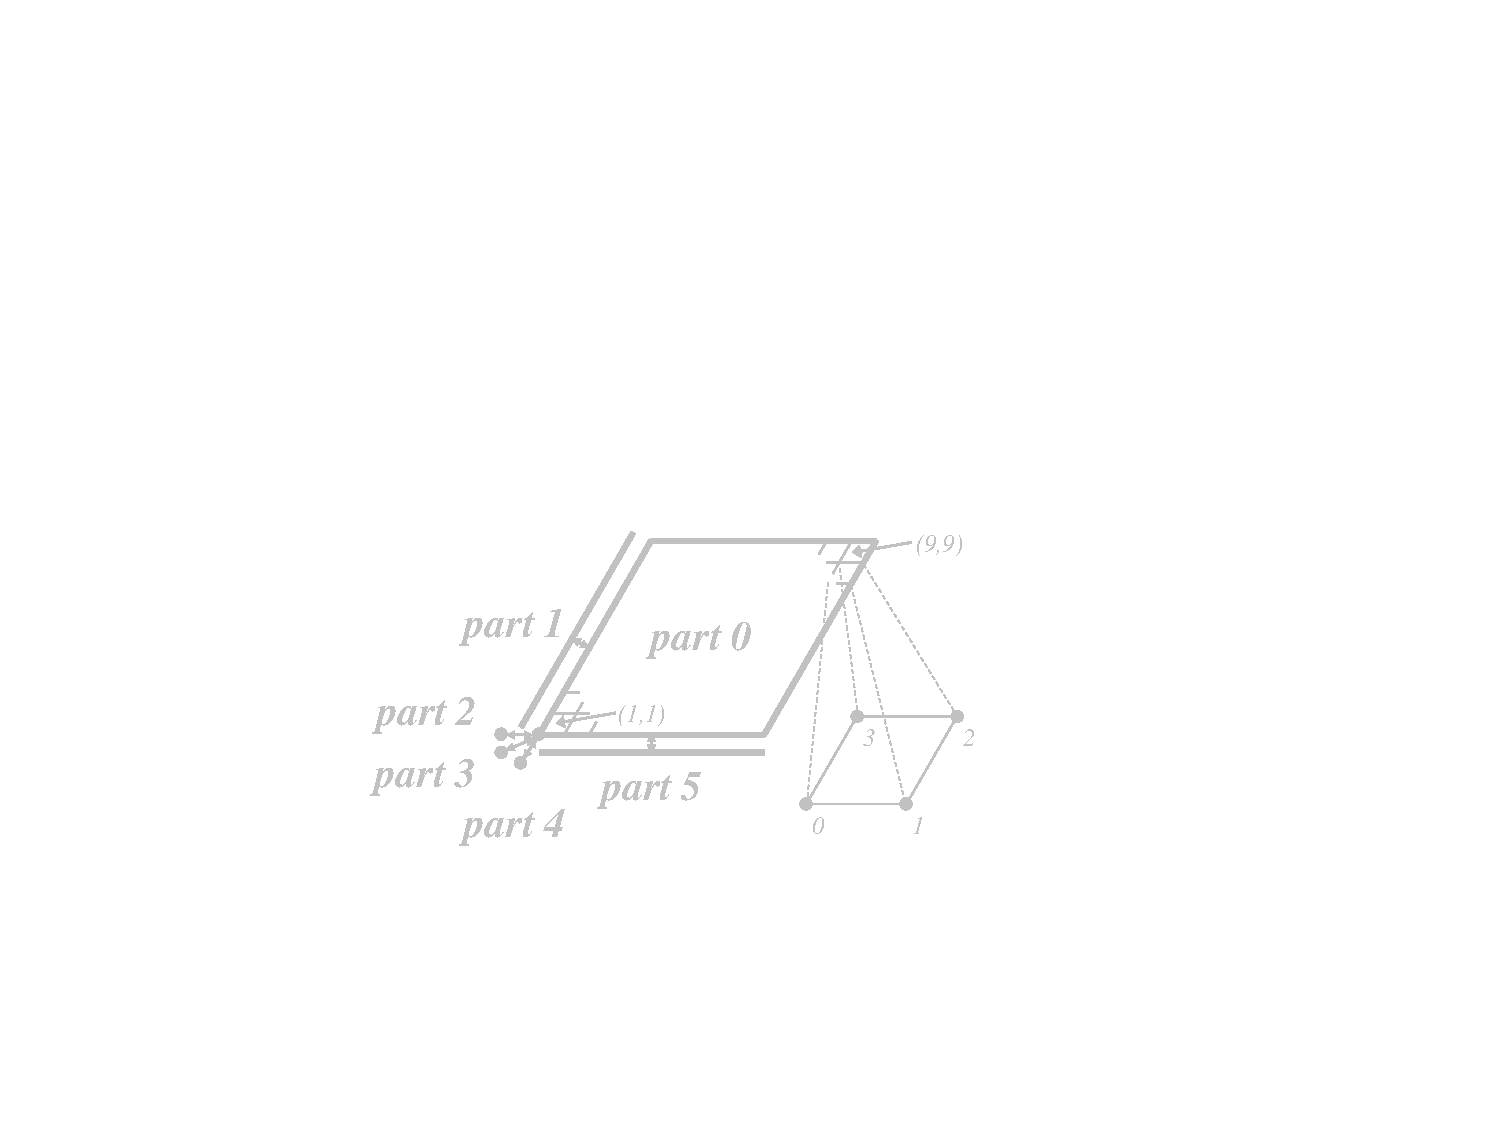
\includegraphics[width=.32\textwidth]{figSStructGridFEM1} \\ 1
\end{tabular}
\hfill
\begin{tabular}{@{}c@{}}
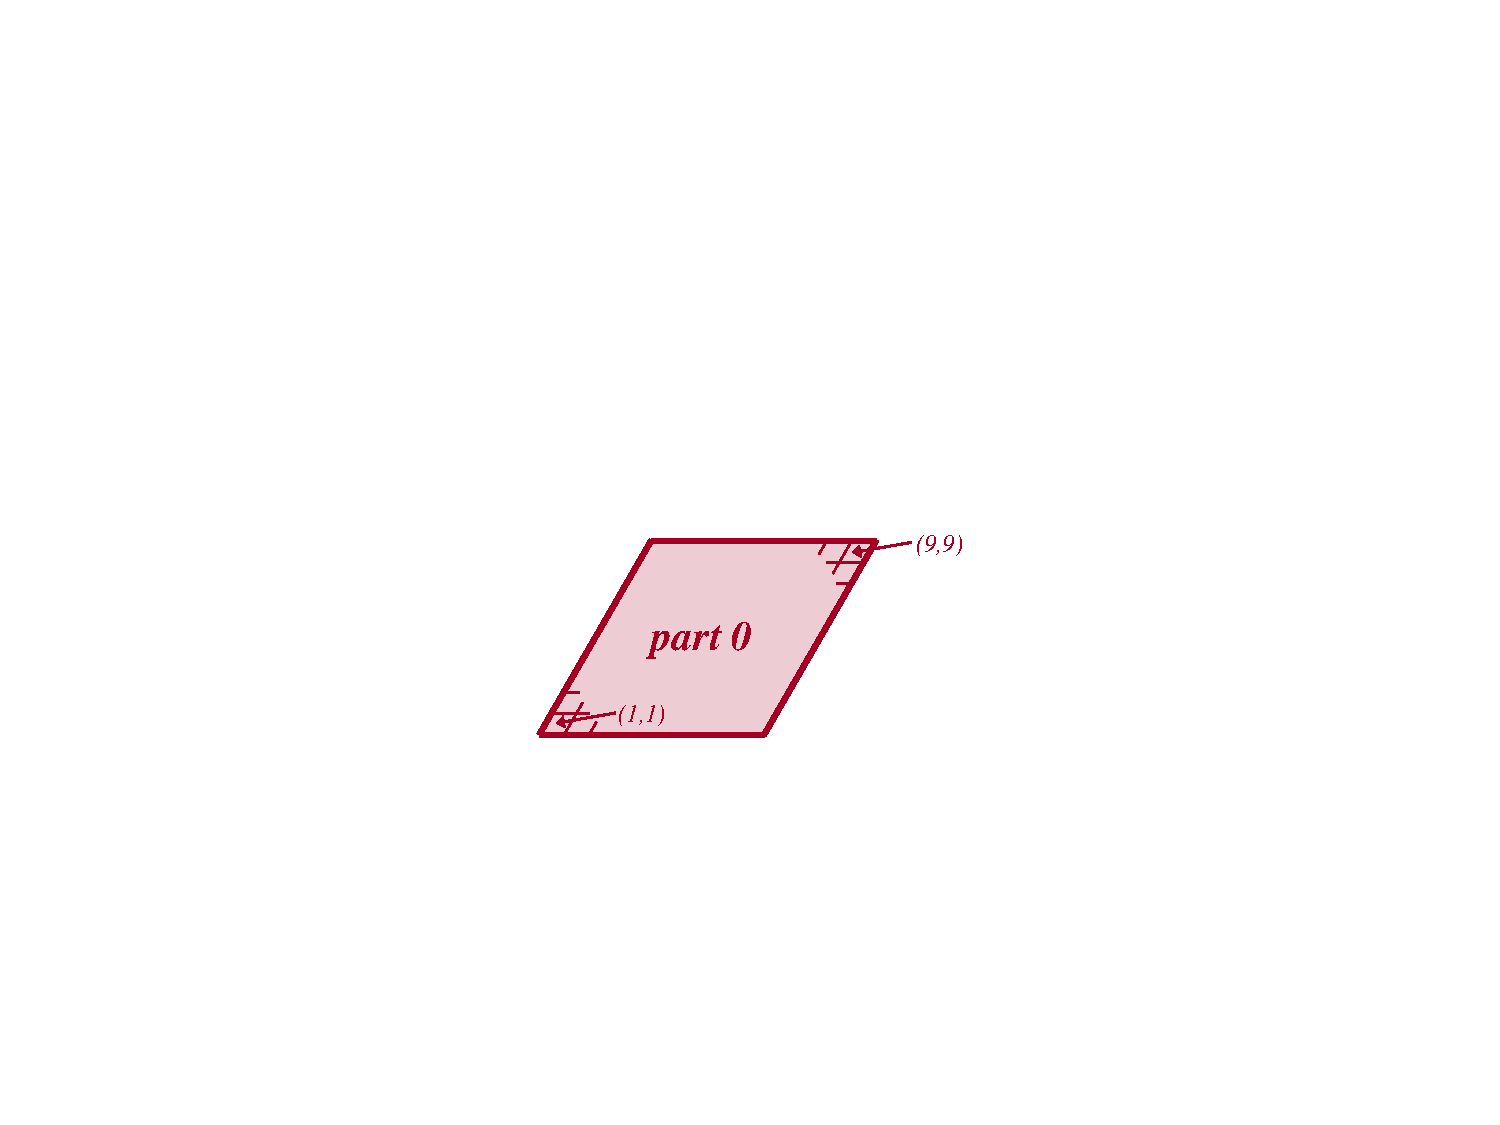
\includegraphics[width=.32\textwidth]{figSStructGridFEM2} \\ 2
\end{tabular}
\hfill
\begin{tabular}{@{}c@{}}
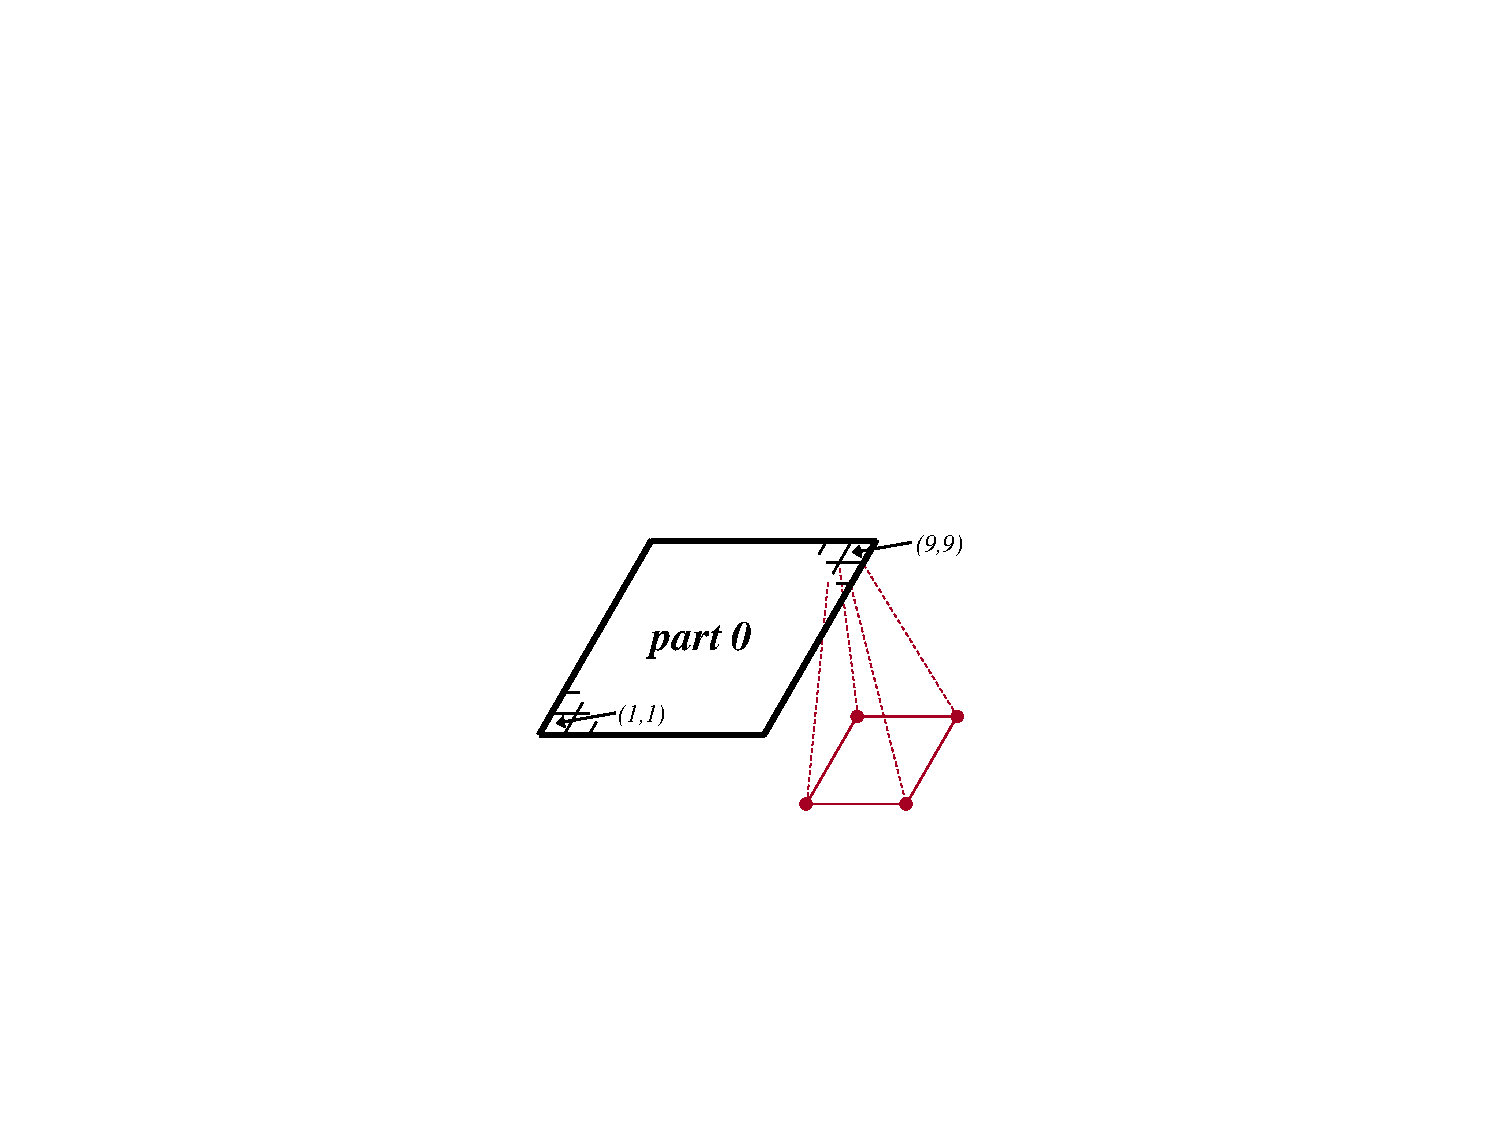
\includegraphics[width=.32\textwidth]{figSStructGridFEM3} \\ 3
\end{tabular}
\vspace{1em} \\
\begin{tabular}{@{}c@{}}
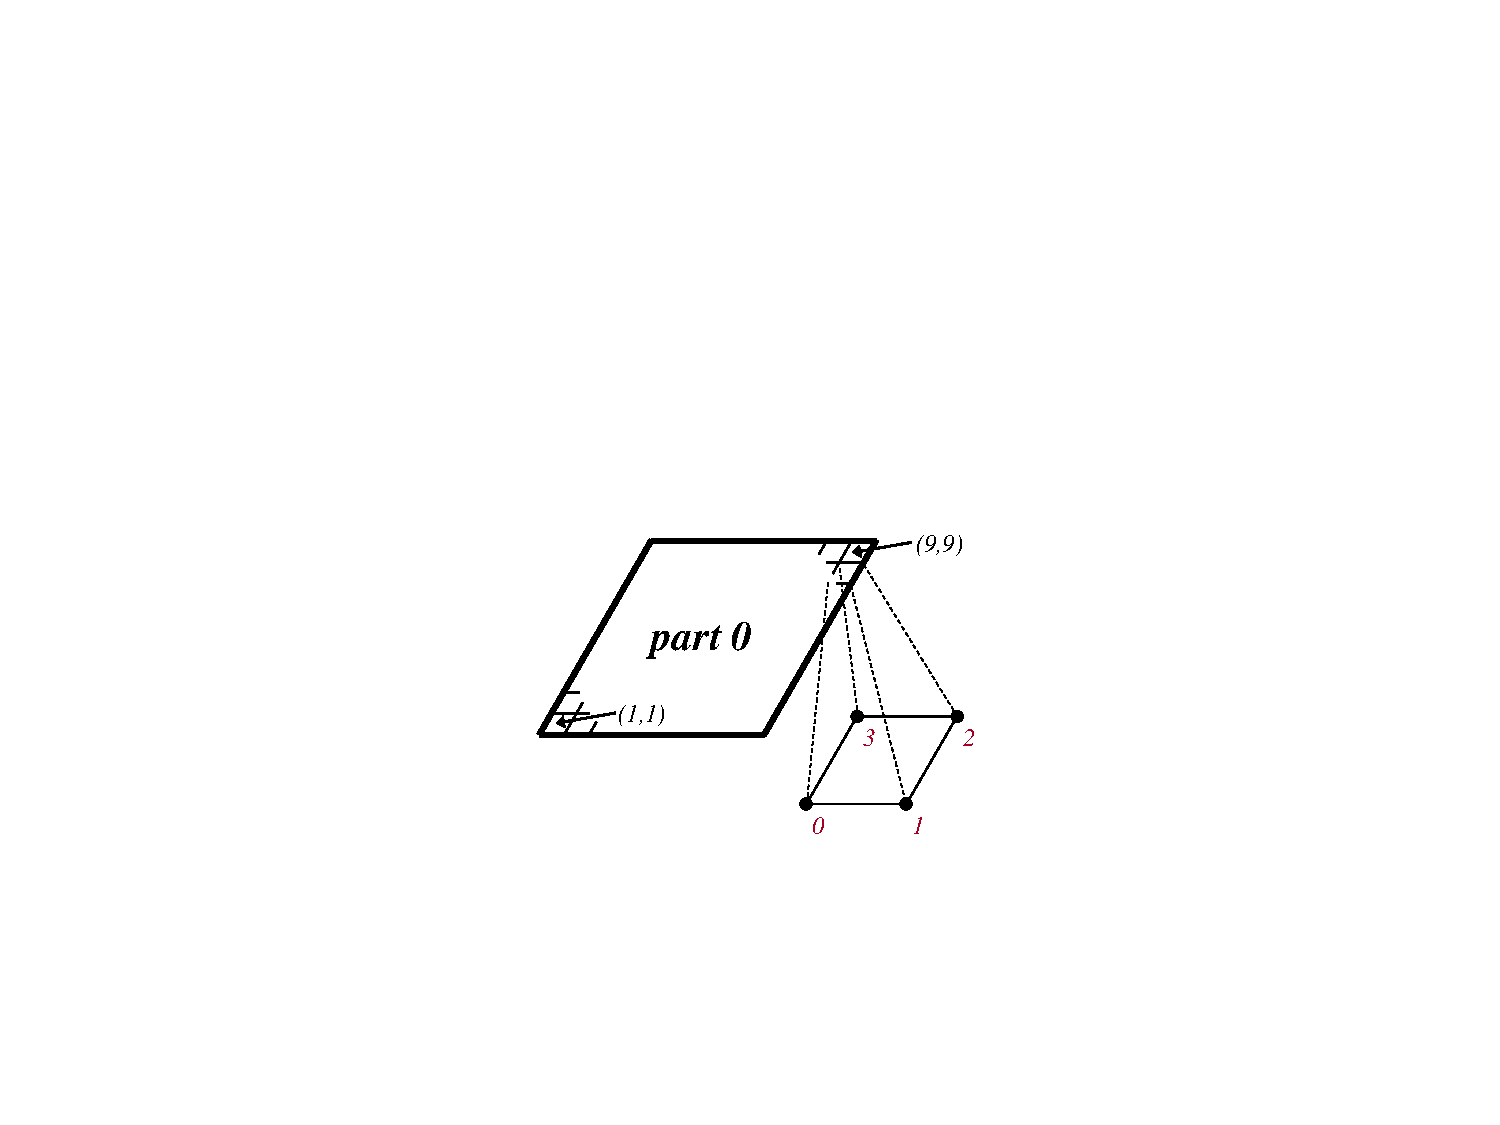
\includegraphics[width=.32\textwidth]{figSStructGridFEM4} \\ 4
\end{tabular}
\hfill
\begin{tabular}{@{}c@{}}
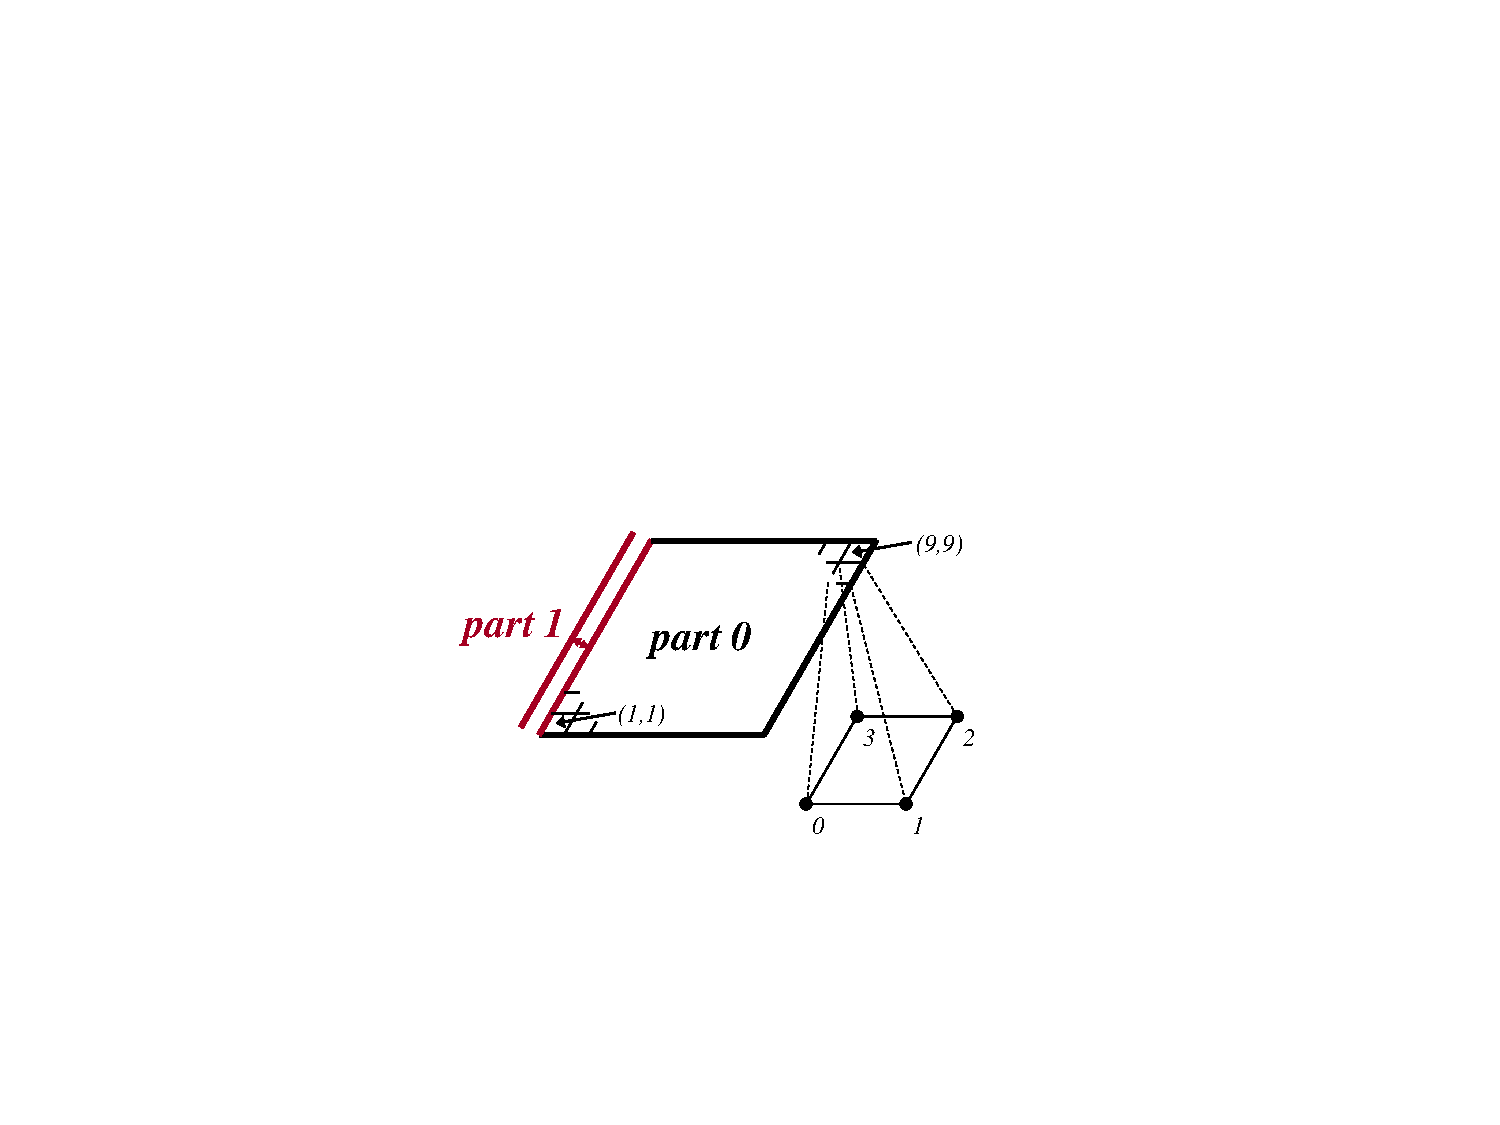
\includegraphics[width=.32\textwidth]{figSStructGridFEM5} \\ 5
\end{tabular}
\hfill
\begin{tabular}{@{}c@{}}
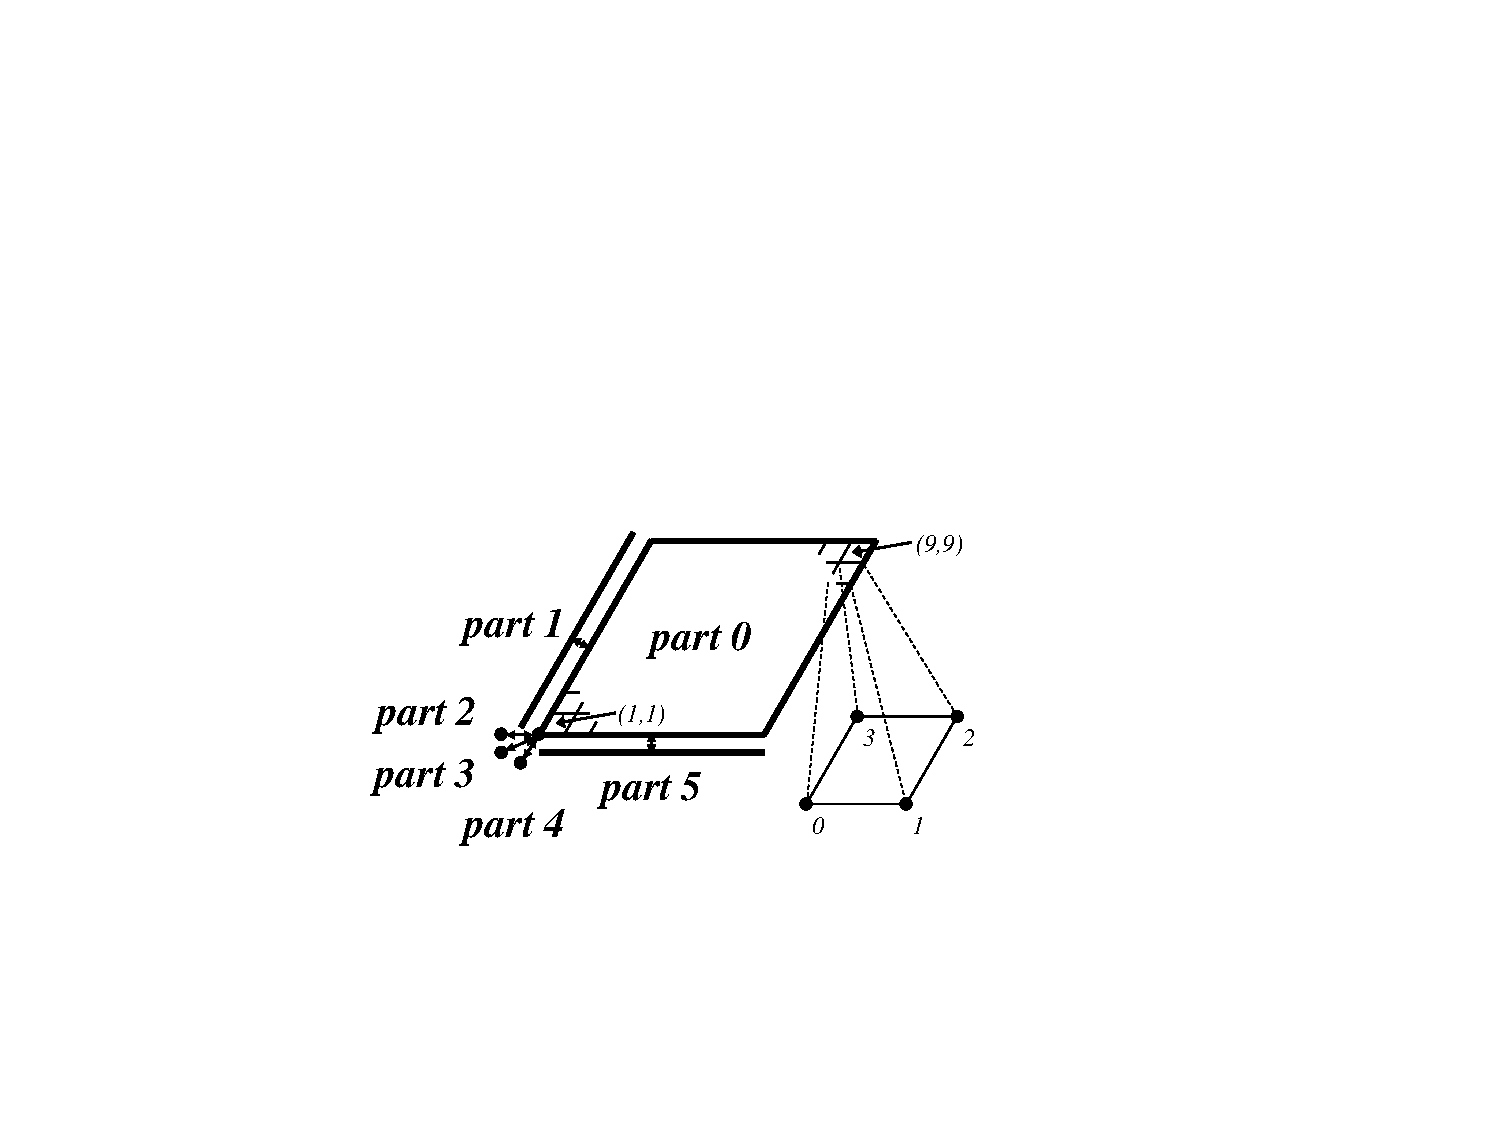
\includegraphics[width=.32\textwidth]{figSStructGridFEM6} \\ 6
\end{tabular}
\vspace{2em} \\
\begin{minipage}{0.9\textwidth}
\begin{verbatim}
    
    HYPRE_SStructGrid grid;
    int ndim = 2, nparts = 6, nvars = 1, part = 0;
    int ilower[2]    = {1,1}, iupper[2] = {9,9};
    int vartypes[]   = {HYPRE_SSTRUCT_VARIABLE_NODE};
    int ordering[12] = {0,-1,-1,  0,+1,-1,  0,+1,+1,  0,-1,+1};

    int s_part   = 2;
    int ilo[2]   = {1,1}, iup[2]   = {1,9}, offset[2]   = {-1,0};
    int s_ilo[2] = {1,1}, s_iup[2] = {9,1}, s_offset[2] = {0,-1};
    int map[2]   = {1,0};
    int dir[2]   = {-1,1};

1:  HYPRE_SStructGridCreate(MPI_COMM_WORLD, ndim, nparts, &grid);
    
    /* Set grid extents, grid variables, and FEM ordering for part 0 */
2:  HYPRE_SStructGridSetExtents(grid, part, ilower, iupper);
3:  HYPRE_SStructGridSetVariables(grid, part, nvars, vartypes);
4:  HYPRE_SStructGridSetFEMOrdering(grid, part, ordering);

    /* Set shared variables for parts 0 and 1 (0 and 2/3/4/5 not shown) */
5:  HYPRE_SStructGridSetSharedPart(grid, part, ilo, iup, offset,
       s_part, s_ilo, s_iup, s_offset, map, dir);

6:  HYPRE_SStructGridAssemble(grid);
    
\end{verbatim}
\end{minipage}
\caption{%
Code on process 0 for setting up the grid in Figure~\ref{fig-sstruct-fem-example}.}
\label{fig-sstruct-fem-grid}
\end{figure}

As in Section~\ref{sec-Block-Structured-Grids}, each process describes that
portion of the grid that it ``owns'', one box at a time.
Figure~\ref{fig-sstruct-fem-grid} shows the code for setting up the grid on
process~0 (the code for the other processes is similar).  The ``icons'' at the
top of the figure illustrate the result of the numbered lines of code.
Process~0 needs to describe the data pictured in the bottom-right of the figure.
That is, it needs to describe part~0 plus some additional information about
shared data with other parts on the grid.  The \code{SetFEMOrdering()} routine
sets the ordering of the unknowns in an element (an element is always a grid
cell in \hypre{}).  This determines the ordering of the data passed into the
routines \code{MatrixAddFEMValues()} and \code{VectorAddFEMValues()} discussed
later.

At this point, the layout of the data on part~0 is complete, but there is no
relationship to the rest of the grid.  To couple the parts, we need to tell
\hypre{} that some of the boundary variables on part~0 are shared with other
parts, i.e., they are the same as some of the variables on other parts.  This is
done through five calls to the \code{SetSharedPart()} routine.  Only the first
call is shown in the figure; the other four calls are similar.  The arguments to
this routine are the same as \code{SetNeighborPart()} with the addition of two
new offset arguments, named \code{offset} and \code{s_offset} in the figure.
Each offset represents a pointer from the cell center to one of the following:
all variables in the cell (no nonzeros in offset); all variables on a face (only
1 nonzero); all variables on an edge (2 nonzeros); all variables at a point (3
nonzeros).  The two offsets must be consistent with each other.

The graph is set up similarly to Figure~\ref{fig-sstruct-graph}, except that the
stencil calls are replaced by calls to \code{GraphSetFEM()}.  The nonzero
pattern of the stiffness matrix can also be set by calling the optional routine
\code{GraphSetFEMSparsity()}.

Matrix and vector values are set one element at a time.  For the example in this
section, calls on part~0 would have the following form:
\begin{verbatim}
   int part = 0;
   int index[2] = {i,j};
   double m_values[16] = {...};
   double v_values[4]  = {...};
   
   HYPRE_SStructMatrixAddFEMValues(A, part, index, m_values);
   HYPRE_SStructVectorAddFEMValues(v, part, index, v_values);
\end{verbatim}
Here, \code{m_values} contains local stiffness matrix values and \code{v_values}
contains local variable values.  The global matrix and vector are assembled
internally by \hypre{}, using the shared variables to couple the parts.

%-----------------------------------------------------------------------------

\section{Structured Adaptive Mesh Refinement}
\label{sec-Structured-Adaptive-Mesh-Refinement}

We now briefly discuss how to use the \code{SStruct} interface in a structured
AMR application.  Consider Poisson's equation on the simple cell-centered
example grid illustrated in Figure \ref{fig-sstruct-samr-grid}.  For structured
AMR applications, each refinement level should be defined as a unique part.
There are two parts in this example: part~0 is the global coarse grid and
part~1 is the single refinement patch.  Note that the coarse unknowns
underneath the refinement patch (gray dots in Figure
\ref{fig-sstruct-samr-grid}) are not real physical unknowns; the solution in
this region is given by the values on the refinement patch.  In setting up the
composite grid matrix \cite{SFMcCormick_1989a} for \hypre{} the equations for
these ``dummy'' unknowns should be uncoupled from the other unknowns (this can
easily be done by setting all off-diagonal couplings to zero in this region).

\begin{figure}
\centering
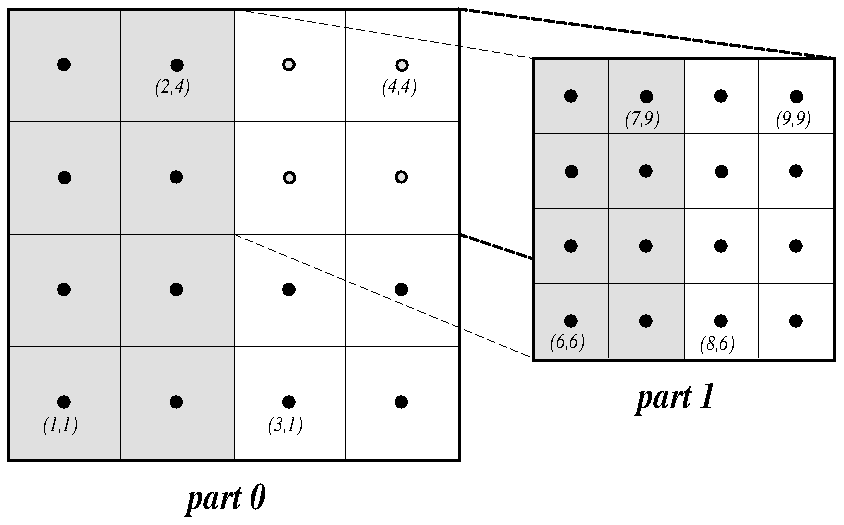
\includegraphics[width=.7\textwidth]{figSStructExample2a}
\caption{%
Structured AMR grid example. Shaded regions correspond to process~0, unshaded
to process~1.  The grey dots are dummy variables.}
\label{fig-sstruct-samr-grid}
\end{figure}

In the example, parts are distributed across the same two processes with
process 0 having the ``left'' half of both parts.  The composite grid is then
set up part-by-part by making calls to \code{GridSetExtents()} just as was done
in Section~\ref{sec-Block-Structured-Grids} and Figure~\ref{fig-sstruct-grid}
(no \code{SetNeighborPart} calls are made in this example).  Note that in the
interface there is no required rule relating the indexing on the refinement
patch to that on the global coarse grid; they are separate parts and thus each
has its own index space.  In this example, we have chosen the indexing such
that refinement cell $(2i,2j)$ lies in the lower left quadrant of coarse cell
$(i,j)$.  Then the stencil is set up.  In this example we are using a finite
volume approach resulting in the standard 5-point stencil in
Figure~\ref{fig-struct-stencil-b} in both parts.

The grid and stencil are used to define all intra-part coupling in the graph,
the non-zero pattern of the composite grid matrix.  The inter-part coupling at
the coarse-fine interface is described by \code{GraphAddEntries()} calls.  This
coupling in the composite grid matrix is typically the composition of an
interpolation rule and a discretization formula.  In this example, we use a
simple piecewise constant interpolation, i.e. the solution value in a coarse
cell is equal to the solution value at the cell center.  Then the flux across a
portion of the coarse-fine interface is approximated by a difference of the
solution values on each side.  As an example, consider approximating the flux
across the left interface of cell $(6,6)$ in Figure
\ref{fig-sstruct-samr-stencil}.  Let $h$ be the coarse grid mesh size, and
consider a local coordinate system with the origin at the center of cell
$(6,6)$.  We approximate the flux as follows
\begin{eqnarray}
\int_{-h/4}^{h/4}{u_x(-h/4,s)} ds
& \approx & \frac{h}{2} u_x(-h/4,0)
  \approx \frac{h}{2} \frac{u(0,0)-u(-3h/4,0)}{3h/4} \\
& \approx & \frac{2}{3} (u_{6,6}-u_{2,3}) \nonumber .
\end{eqnarray} 
The first approximation uses the midpoint rule for the edge integral, the second
uses a finite difference formula for the derivative, and the third the piecewise
constant interpolation to the solution in the coarse cell.  This means that the
equation for the variable at cell $(6,6)$ involves not only the stencil
couplings to $(6,7)$ and $(7,6)$ on part~1 but also non-stencil couplings to
$(2,3)$ and $(3,2)$ on part~0.  These non-stencil couplings are described by
\code{GraphAddEntries()} calls.  The syntax for this call is simply the part and
index for both the variable whose equation is being defined and the variable to
which it couples.  After these calls, the non-zero pattern of the matrix (and
the graph) is complete.  Note that the ``west'' and ``south'' stencil couplings
simply ``drop off'' the part, and are effectively zeroed out (currently, this is
only supported for the \code{HYPRE_PARCSR} object type, and these values must be
manually zeroed out for other object types; see \code{MatrixSetObjectType()} in
the reference manual).

\begin{figure}
\centering
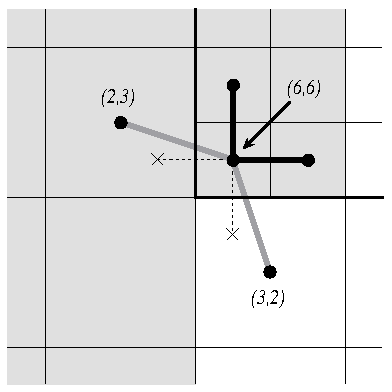
\includegraphics[width=.4\textwidth]{figSStructExample2b}
\caption{%
Coupling for equation at corner of refinement patch. Black lines
(solid and broken) are stencil couplings. Gray line are non-stencil
couplings.}
\label{fig-sstruct-samr-stencil}
\end{figure}

The remaining step is to define the actual numerical values for the composite
grid matrix.  This can be done by either \code{MatrixSetValues()} calls to set
entries in a single equation, or by \code{MatrixSetBoxValues()} calls to set
entries for a box of equations in a single call.  The syntax for the
\code{MatrixSetValues()} call is a part and index for the variable whose
equation is being set and an array of entry numbers identifying which entries
in that equation are being set.  The entry numbers may correspond to stencil
entries or non-stencil entries.

\chapter{Finite Element Interface}
\label{ch-FEI}

\section{Introduction}

Many application codes use unstructured finite element meshes.
This section describes an interface for finite element problems,
called the {\tt FEI}, which is supported in \hypre{}.
\begin{figure}[htbp]
\centerline{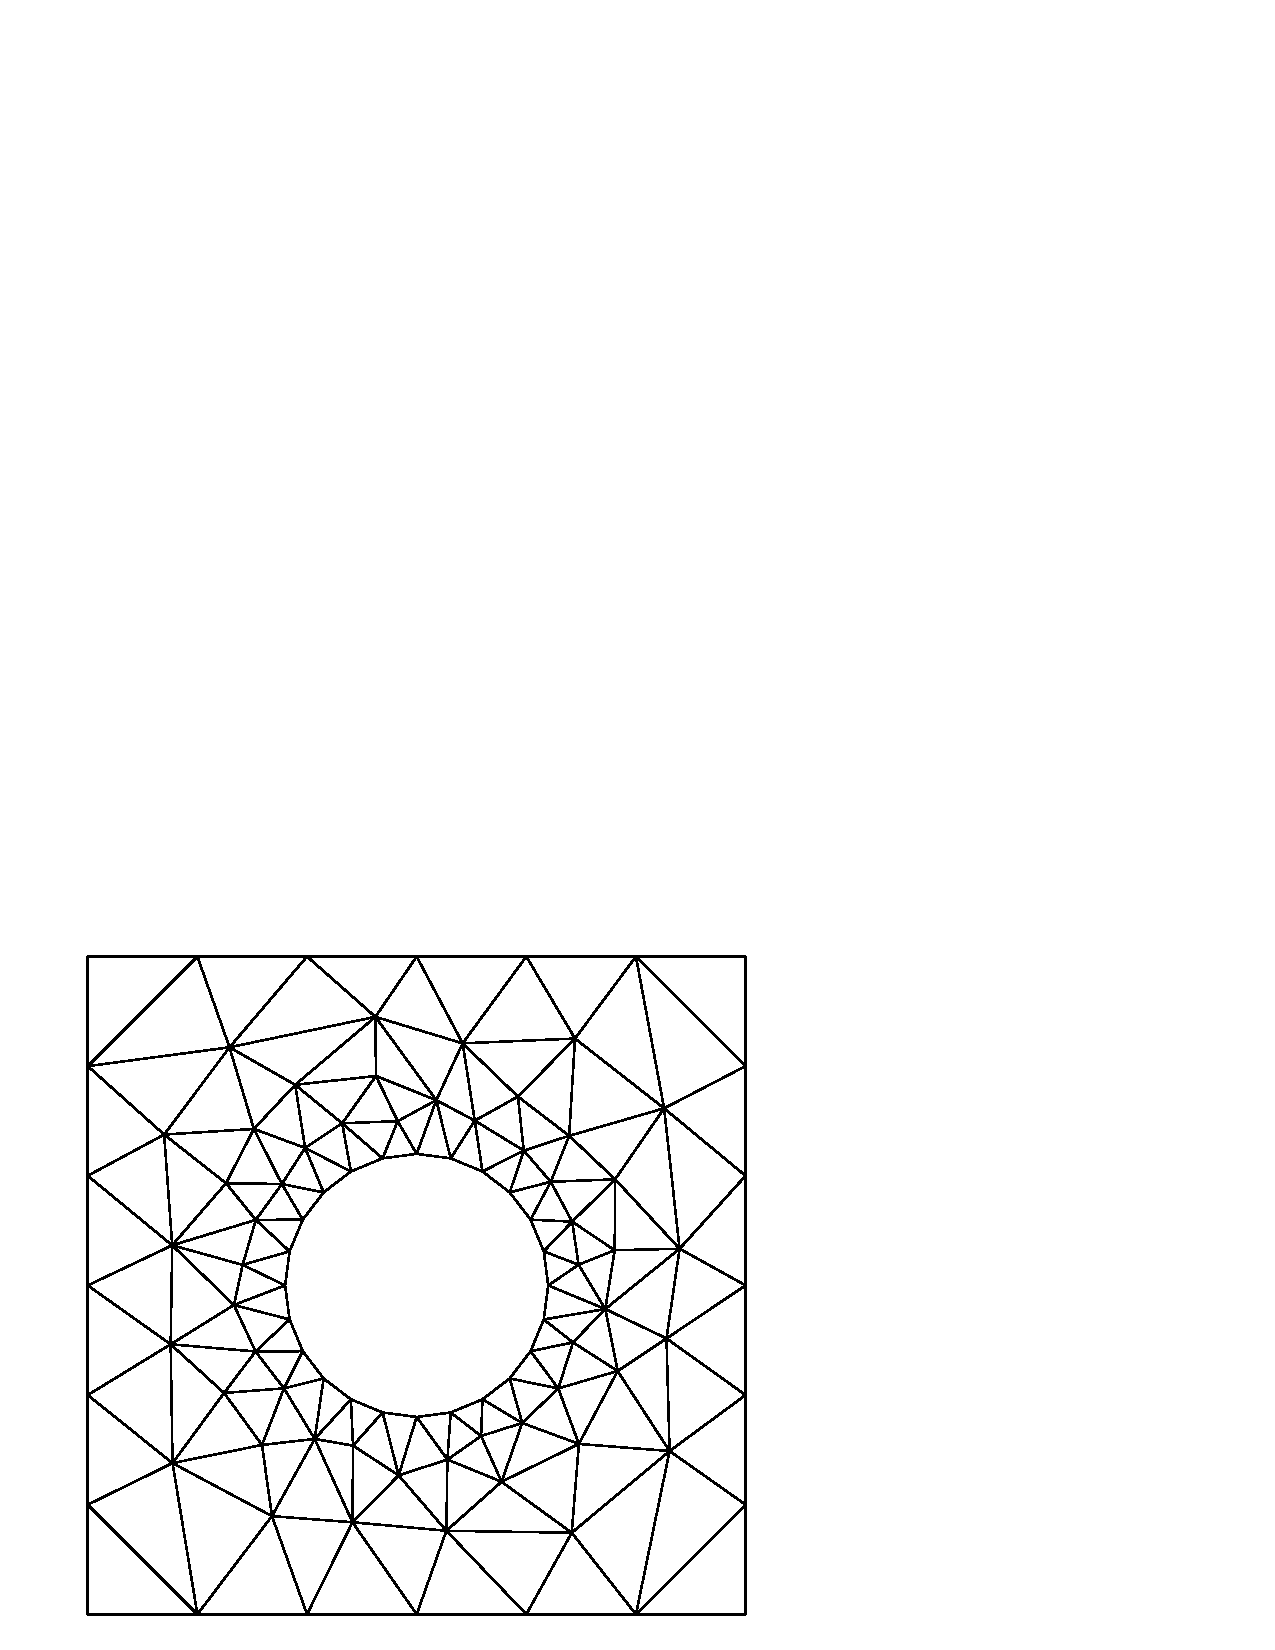
\includegraphics[width=.3\textwidth]{square-hole.pdf}}
\caption{Example of an unstructured mesh.}
\end{figure}

{\tt FEI} refers to a specific interface for black-box finite element
solvers, originally developed in Sandia National Lab, see \cite{FEI-ref}.
It differs from the rest of the conceptual interfaces in
\hypre{} in two important aspects: it is written in C++, and
it does not separate the construction of the linear system matrix
from the solution process.
A complete description of Sandia's {\tt FEI} implementation can be obtained
by contacting Alan Williams at Sandia (william@sandia.gov).
A simplified version of the {\tt FEI} has been implemented
at LLNL and is included in \hypre{}.
More details about this implementation can be found in the header
files of the \code{FEI_mv/fei-base} and \code{FEI_mv/fei-hypre} directories.

%% The purpose of the {\tt FEI} is to allow users to submit the global
%% matrices in the form of element connectivities, element stiffness matrices,
%% element loads, and boundary conditions.
%% The element information is processed by an implementation of the
%% {\tt FEI} (see \cite{FEI-ref}) which loads the global matrix and right
%% hand side vectors to the linear solver libraries via the
%% {\tt LinearSystemCore} interface.

%% In the next section, we 
%% describe the basic {\tt FEI} functions and a sample program to 
%% demonstrate how to use them. 


%% User applications access the \hypre{} linear solvers via a pipeline of
%% two interfaces - user to finite element interface (called {\tt FEI}),
%% and the finite element to linear solver interface (called 
%% {\tt LinearSystemCore}). The purpose of {\tt FEI} is to allow users 
%% to submit the global matrices in the form of element connectivities, 
%% element stiffness matrices, element loads, and boundary conditions. 
%% The element information is processed by an implementation of the 
%% {\tt FEI} (see \cite{FEI-ref}) which loads the global matrix and right
%% hand side vectors to the linear solver libraries via the 
%% {\tt LinearSystemCore} interface.
%% The {\tt LinearSystemCore} interface also facilitates interfacing 
%% multiple linear system solver packages (such as PetSC or Aztec)
%% with little change in the user code. Users interact with an FEI
%% solver primarily at the FEI level.

%% The specification of the {\tt FEI} and its implementation was first
%% developed at Sandia. A simplified implementation has been implemented
%% at LLNL in \hypre{}'s finite element module. While most of \hypre{}
%% is written in C, the {\tt FEI} and {\tt LinearSystemCore}
%% interfaces are written in C++. In the next section, we 
%% describe the basic {\tt FEI} functions and a sample program to 
%% demonstrate how to use them. 

%A brief description of \hypre{}'s 
%internal data structure and solver capabilities is presented in 
%Section 5.3.  Associated with \hypre{}'s finite element interface is 
%an FE-based gray-box multilevel preconditioning module called 
%{\tt MLI} which provides fast multilevel preconditioners.
%A description of the {\tt MLI} is given in Section 5.4.
%In Section 5.5, we describe the available options for using \hypre{}'s
%rich solver capabilities. 
%Users who prefer to create their own finite
%element packages but would like to use the \hypre{} solvers can link their
%packages to \hypre{} via the {\tt LinearSystemCore}. A description
%of this interface is given in Section \ref{LSI_overview}. Some installation 
%and usage issues are discussed in Section \ref{LSI_install}.

\section{A Brief Description of the Finite Element Interface}

Typically, finite element codes contain data structures storing element
connectivities, element stiffness matrices, element loads, boundary conditions,
nodal coordinates, etc.
One of the purposes of the {\tt FEI} is to assemble the global linear
system in parallel based on such local element data.
We illustrate this in the rest of the section and refer to example 10
(in the \code{examples} directory) for more implementation details.

In \hypre{}, one creates an instance of the {\tt FEI} as follows:
\begin{display}
\begin{verbatim}
LLNL_FEI_Impl *feiPtr = new LLNL_FEI_Impl(mpiComm);
\end{verbatim}
\end{display}
Here {\tt mpiComm} is an MPI communicator (e.g. {\tt MPI\_COMM\_WORLD}).
If Sandia's {\tt FEI} package is to be used, one needs to define
a \hypre{} solver object first:
\begin{display}
\begin{verbatim}
LinearSystemCore   *solver = HYPRE_base_create(mpiComm);
FEI_Implementation *feiPtr = FEI_Implementation(solver,mpiComm,rank);
\end{verbatim}
\end{display}
where {\tt rank} is the number of the master processor (used only
to identify which processor will produce the screen outputs).
The \code{LinearSystemCore} class is the part of the \code{FEI} which
interfaces with the linear solver library. It will be discussed later in
Sections \ref{LSI_solvers} and \ref{LSI_install}.

Local finite element information is passed to the {\tt FEI} using
several methods of the \code{feiPtr} object.
The first entity to be submitted is the {\it field} information. 
A {\it field} has an identifier called {\tt fieldID} and a rank or
{\tt fieldSize} (number of degree of freedom). For example, a discretization
of the Navier Stokes equations in 3D can consist of velocity vector having
$3$ degrees of freedom in every node (vertex) of the mesh and a scalar pressure
variable, which is constant over each element. If these are the only variables,
and if we assign {\tt fieldID}s $7$ and $8$ to them, respectively, then the
finite element field information can be set up by
\begin{display}
\begin{verbatim}
nFields   = 2;                 /* number of unknown fields */
fieldID   = new int[nFields];  /* field identifiers */
fieldSize = new int[nFields];  /* vector dimension of each field */

/* velocity (a 3D vector) */
fieldID[0]   = 7;
fieldSize[0] = 3;

/* pressure (a scalar function) */
fieldID[1]   = 8;
fieldSize[1] = 1;

feiPtr -> initFields(nFields, fieldSize, fieldID);
\end{verbatim}
\end{display}

Once the field information has been established, we are ready to initialize
an element block. An element block is characterized by the block identifier,
the number of elements, the number of nodes per element, the nodal fields 
and the element fields (fields that have been defined previously). Suppose 
we use $1000$ hexahedral elements in the element block $0$, the setup 
consists of
\begin{display}
\begin{verbatim}
elemBlkID  = 0;     /* identifier for a block of elements */
nElems     = 1000;  /* number of elements in the block */
elemNNodes = 8;     /* number of nodes per element */

/* nodal-based field for the velocity */
nodeNFields     = 1;
nodeFieldIDs    = new[nodeNFields];
nodeFieldIDs[0] = fieldID[0];

/* element-based field for the pressure */
elemNFields     = 1;
elemFieldIDs    = new[elemNFields];
elemFieldIDs[0] = fieldID[1];

feiPtr -> initElemBlock(elemBlkID, nElems, elemNNodes, nodeNFields,
                        nodeFieldIDs, elemNFields, elemFieldIDs, 0);
\end{verbatim}
\end{display}
The last argument above specifies how the dependent variables are arranged in
the element matrices. A value of $0$ indicates that each variable is to be
arranged in a separate block (as opposed to interleaving).

In a parallel environment, each processor has one or more element blocks.
Unless the element blocks are all disjoint, some of them
share a common set of nodes on the subdomain boundaries. To facilitate
setting up interprocessor communications, shared nodes between subdomains
on different processors are to be identified and sent to the {\tt FEI}.
Hence, each node in the whole domain is assigned a unique global
identifier. The shared node list on each processor contains a subset
of the global node list
corresponding to the local nodes that are shared with the other processors.
The syntax for setting up the shared nodes is
\begin{display}
\begin{verbatim}
feiPtr -> initSharedNodes(nShared, sharedIDs, sharedLengs, sharedProcs);
\end{verbatim}
\end{display}
This completes the initialization phase, and a completion signal is sent to
the {\tt FEI} via
\begin{display}
\begin{verbatim}
feiPtr -> initComplete();
\end{verbatim}
\end{display}

Next, we begin the {\it load} phase. The first entity for loading is the
nodal boundary conditions. Here we need to specify the number of boundary
equations and the boundary values given by {\tt alpha, beta}, and {\tt gamma}.  Depending on whether the boundary conditions are Dirichlet, Neumann, or mixed,
the three values should be passed into the {\tt FEI} accordingly. 
\begin{display}
\begin{verbatim}
feiPtr -> loadNodeBCs(nBCs, BCEqn, fieldID, alpha, beta, gamma);
\end{verbatim}
\end{display}
The element stiffness matrices are to be loaded in the next step. We need
to specify the element number $i$, the element block to which element $i$
belongs, the element connectivity information, the element load, and the
element matrix format. The element connectivity specifies a set of $8$ node
global IDs (for hexahedral elements), and the element load is the load or
force for each degree of freedom.  The element format specifies how the
equations are arranged (similar to the interleaving scheme mentioned above).
The calling sequence for loading element stiffness matrices is
\begin{display}
\begin{verbatim}
for (i = 0; i < nElems; i++)
   feiPtr -> sumInElem(elemBlkID, elemID, elemConn[i], elemStiff[i],
                       elemLoads[i], elemFormat);
\end{verbatim}
\end{display}
To complete the assembling of the global stiffness matrix and the
corresponding right hand side, a signal is sent to the {\tt FEI} via
\begin{display}
\begin{verbatim}
feiPtr -> loadComplete();
\end{verbatim}
\end{display}

%% \section{The Finite Element Interface Matrix and Vector Classes}

%% This section describes two additional classes (other than {\tt HYPRE\_FEMesh})
%% that users may need - {\tt HYPRE\_FEMatrix} and {\tt HYPRE\_FEVector}. 
%% These classes are useful if the global finite element stiffness matrix is
%% to be solved using solvers other than those available via the finite element
%% interface. The key task is to extract
%% the matrix and vector internal to the {\tt FEI}. The matrix can be extracted
%% by first instantiating an {\tt HYPRE\_FEMatrix} object
%% \begin{tabbing}
%% \hspace{0.5in} \= {\tt HYPRE\_FEMatrixCreate(mpiComm, hypreMesh, \&feMatrix);}
%% \end{tabbing}
%% where {\tt hypreMesh} is the object created before, and {\tt feMatrix} is 
%% the pointer to the new object.
%% The \hypre{} matrix in {\tt ParCSR} format can then be extracted by
%% \begin{tabbing}
%% \hspace{0.5in} \= {\tt HYPRE\_FEMatrixGetObject(feMatrix, (void **) \&parcsrMatrix);}
%% \end{tabbing}
%% Similarly, the right hand side vector can be extracted by
%% \begin{tabbing}
%% \hspace{0.5in} \= {\tt HYPRE\_FEVectorCreate(mpiComm, hypreMesh, \&feVector);}
%% \end{tabbing}
%% and
%% \begin{tabbing}
%% \hspace{0.5in} \= {\tt HYPRE\_FEVectorGetRHS(feMatrix, (void**) \&parVectorRHS);}
%% \end{tabbing}
%% When the solution of the linear system is obtained, it can be given
%% to the {\tt FEI} by
%% \begin{tabbing}
%% \hspace{0.5in} \= {\tt HYPRE\_FEVectorSetSol(feMatrix, (void*) parVectorSol);}
%% \end{tabbing}
%% Finally, the objects are destroyed by the corresponding destroy functions.

%\section{The LinearSystemCore Interface}
%\label{LSI_overview}

%As described before, users who prefer to create their own finite element
%interface package can also take advantage of the rich solver capabilities
%in \hypre{}. In this section we show how to access {\tt HYPRE\_LinSysCore}'s
%internal solver directly.  
%The matrix class in \hypre{} accessible via the {\tt LinearSystemCore} interface
%is the parallel compressed sparse row ({\tt ParCSR}) matrix.  The
%requirements about how the global matrix is partitioned among the
%processors are that each processor holds a contiguous block of rows and columns
%and the equation numbers in processors of lower rank are lower than those
%in processors of higher rank.  The {\tt FEI} is responsible for ensuring
%that these two requirements are followed. The matrix can be loaded in
%parallel - a row or a block of rows at a time.  The solution and right
%hand side vectors are constructed accordingly. The matrix rows corresponding
%to the shared nodes can be assigned to either processor, and is determined
%by the {\tt FEI} itself. Once the incoming matrix and vector data have
%been captured in the \hypre{} {\tt ParCSR} format, a whole of matrix and
%vector operators are available for use in the \hypre{} solvers.
%
%The following program segment describes the function calls to set up
%the internal matrix and solve the linear system.
%Users need first to 
%construct an array (say, {\tt eqnOffsets} describing the matrix row
%partitioning across all processors (so {\tt eqnOffsets[p]} and
%{\tt eqnOffset[p+1]} have the starting and ending row indices for processor
%p). Furthermore, suppose the local submatrix has been constructed as a
%compressed sparse row (CSR) matrix in the {\tt ia, ja, val} arrays. 
%
%\begin{tabbing}
%\hspace{0.5in} \= {\tt Program Segment} \\[1mm]
%\> {\tt startRow = eqnOffsets[mypid];} \\
%\> {\tt endRow = eqnOffsets[mypid+1] - 1;} \\
%\> {\tt nrows = endRow - startRow + 1} \\
%\> {\tt for ( i = startRow; i $<=$ endRow; i++ ) $\{$ } \\
%\> \hspace{0.3in} \= {\tt ncnt = ia[i+1] - ia[i];} \\
%\> \> {\tt rowLengths[i-startRow] = ncnt;} \\
%\> \> {\tt colIndices[i-startRow] = new int[ncnt];} \\
%\> \> {\tt k = 0;} \\
%\> \> {\tt for (j = ia[i]; j < ia[i+1]; j++) colIndices[i-startRow][k++] = ja[j];}\\
%\> \} \\
%\> {\tt HYPRE\_LinSysCore\_create(\&lsc, MPI\_COMM\_WORLD);} \\
%\> {\tt HYPRE\_setGlobalOffsets(lsc, nrows, NULL, eqnOffsets, NULL);} \\
%\> {\tt HYPRE\_setMatrixStructure(lsc, colIndices, rowLengths, NULL, NULL, NULL);} \\
%\> {\tt for ( i = startRow; i <= endRow; i++ ) $\{$ } \\
%\> \> {\tt ncnt = ia[i+1] - ia[i];} \\
%\> \> {\tt HYPRE\_sumIntoSystemMatrix(lsc, i, ncnt, \&val[ia[i]], \&ja[ia[i]]);}\\
%\> \> {\tt HYPRE\_sumIntoRHSVector(1, \&rhs[i], \&i);} \\
%\> \} \\
%\> {\tt HYPRE\_matrixLoadComplete();}\\
%\> {\tt strcpy(paramString, "solver gmres");} \\
%\> {\tt HYPRE\_parameters(1, \&paramString);} \\
%\> {\tt strcpy(paramString, "preconditioner boomeramg");} \\
%\> {\tt HYPRE\_parameters(1, \&paramString);} \\
%\> {\tt HYPRE\_launchSolver(\&status, \&iterations);}
%\end{tabbing}

%A list of available functions is given in the reference manual.
%
%\begin{tabbing}
%{\tt HYPRE\_LinSysCore\_create(LinSysCore **lsc, MPI\_Comm comm)} \\[1mm]
%{\tt HYPRE\_LinSysCore\_destroy(LinSysCore **lsc)} \\[1mm]
%{\tt HYPRE\_parameters(LinSysCore *lsc, int nParams, char **params)} \\[1mm]
%{\tt HYPRE\_setGlobalOffsets(LinSysCore* lsc, int leng, int* nodeOffsets,} \\
%\hspace{1.0in} {\tt int* eqnOffsets, int* blkEqnOffsets)} \\[1mm]
%{\tt HYPRE\_setMatrixStructure(LinSysCore *lsc, int** ptColIndices,} \\
%\hspace{1.0in} {\tt int* ptRowLengths, int** blkColIndices, int* blkRowLengths, int* ptRowsPerBlkRow)} \\[1mm]
%{\tt HYPRE\_resetMatrixAndVector(LinSysCore *lsc, double val)} \\[1mm]
%{\tt HYPRE\_resetMatrix(LinSysCore *lsc, double val)} \\[1mm]
%{\tt HYPRE\_resetRHSVector(LinSysCore *lsc, double val)} \\[1mm]
%{\tt HYPRE\_sumIntoSystemMatrix(LinSysCore *lsc, int numPtRows, const int* ptRows,}\\
%\hspace{1.0in} {\tt int numPtCols, const int* ptCols, int numBlkRows, const int* blkRows,} \\
%\hspace{1.0in} {\tt int numBlkCols, const int* blkCols, const double* const* values)} \\[1mm]
%{\tt HYPRE\_sumIntoRHSVector(LinSysCore *lsc, int num, const double* values, const int* indices)} \\[1mm]
%{\tt HYPRE\_matrixLoadComplete(LinSysCore *lsc)} \\[1mm]
%{\tt HYPRE\_enforceEssentialBC(LinSysCore *lsc, int* globalEqn, double* alpha,
%                             double* gamma, int leng)} \\[1mm]
%
%{\tt HYPRE\_enforceRemoteEssBCs(LinSysCore *lsc,int numEqns,int* globalEqns, int** colIndices,} \\
%\hspace{1.0in} {\tt int* colIndLen, double** coefs)} \\[1mm]

%{\tt HYPRE\_enforceOtherBC(LinSysCore *lsc, int* globalEqn, double* alpha, double *beta} \\
%\hspace{1.0in} {\tt double* gamma, int leng)} \\[1mm]

%{\tt HYPRE\_putInitialGuess(LinSysCore *lsc, const int* eqnNumbers,
%                          const double* values, int leng)} \\[1mm]
%{\tt HYPRE\_getSolution(LinSysCore *lsc, double *answers, int leng)} \\[1mm]

%{\tt HYPRE\_getSolnEntry(LinSysCore *lsc, int eqnNumber, double *answer)} \\[1mm]

%{\tt HYPRE\_formResidual(LinSysCore *lsc, double *values, int leng)} \\[1mm]

%{\tt HYPRE\_launchSolver(LinSysCore *lsc, int *solveStatus, int *iter)} \\[1mm]
%\end{tabbing}

%\section{HYPRE LinearSystemCore Installation}
%
%The ultimate objective is for application users to have immediate access
%to the latest FEI/\hypre{} library files on different computing platforms
%via public {\tt lib} directories.  While this feature is forthcoming, careful 
%version control is needed for users to keep track of capabilities and bug fixes 
%for different installations.  Users who would like to set up the FEI/\hypre{}
%on their own should do the following :
%
%\begin{enumerate}
%
%\item obtain the \hypre{} and the Sandia FEI source codes (alternatively, use
%      the {\tt FEI} implementation in \hypre{}),
%\item compile Sandia's {\tt FEI} (fei-2.5.0) to create the
%      {\tt libfei\_base.a} file.
%\item compile \hypre{} 
%\begin{enumerate}
%\item download \hypre{} from the web, ungzip and untar it
%\item go into the {\tt linear\_solvers} directory
%\item do a 'configure' with the {\tt --with-fei-inc-dir} option set to
%      the {\tt FEI} include directory plus other compile options
%\item compile with {\tt make install} to create the
%      {\tt libHYPRE\_LSI*} file in the {\tt linear\_solvers/hypre/lib}
%      directory.
%\end{enumerate}
%\item call the {\tt FEI} functions in your application code (example given
%      previously)
%\begin{enumerate}
%\item include {\tt cfei\-hypre.h} in your file 
%\item include {\tt FEI\_Implementation.h} in your file 
%\item make sure your application has an {\tt include} and an {\tt lib} path 
%      to the {\tt include} and {\tt lib} directories created above. 
%\end{enumerate}
%
%\end{enumerate}
%
%%\subsection{Linking with the library files}
%
%To link the {\tt FEI} and \hypre{} into the executable, the following has to be
%attached to the linking command :
%
%\begin{tabbing}
%\hspace{0.5in} \= {\tt -L\$$\{$LIBPATHS$\}$ -lfei\_base -lHYPRE\_LSI} 
%\end{tabbing}
%along with all the other libraries (Note : the order in which the libraries are
%listed may be important), where {\tt LIBPATHS} are where 
%the \hypre{} and {\tt FEI} libraray files can be found.  
%
%Since some of these library files make calls to LAPACK and BLAS functions, 
%the corresponding libraries need to be linked along with (placed after) these 
%library files.  
%%For example, on the DEC cluster, it suffices to link
%%with the {\tt dxml} library, (So {\tt -ldxml} is placed after the above link
%%sequence, with {\tt -lm} placed after {\tt -ldxml}.) while the {\it essl}
%%library can be used on the blue machine. If {\tt SuperLU} is also needed,
%%{\tt -lHYPRE\_superlu} should be placed immediately after {\tt HYPRE\_LSI}.
%
%%\subsection{Some more caveats for application developers}
%
%Building an application executable often requires linking with many different
%software packages, and many software packages use some LAPACK and/or BLAS
%functions.  In order to alleviate the problem of multiply defined functions
%at link time, it is recommended that all software libraries are stripped of
%all LAPACK and BLAS function definitions.  These LAPACK and BLAS functions 
%should then be resolved at link time by linking with the system LAPACK and
%BLAS libraries (e.g. dxml on DEC cluster).  Both \hypre{} and SuperLU were
%built with this in mind.  However, some other software library files needed
%may have the BLAS functions defined in them.  To avoid the problem of
%multiply defined functions, it is recommended that the offending library
%files be stripped of the BLAS functions.
%
%%\subsection{Comments about the FEI/\hypre{} Interface and Contacts}
%
%%Comments about \hypre{}'s finite element interface can be directed
%%to Charles Tong (925-422-3411, chtong@llnl.gov).
%

%=============================================================================
%=============================================================================

\chapter{Linear-Algebraic System Interface (IJ)}
\label{ch-IJ}

The \code{IJ} interface described in this chapter is the lowest common
denominator for specifying linear systems in \hypre{}.  This interface
provides access to general sparse-matrix solvers in \hypre{}, not
to the specialized solvers that require more problem information.

%-----------------------------------------------------------------------------

\section{IJ Matrix Interface}

As with the other interfaces in \hypre{}, the \code{IJ} interface
expects to get data in distributed form because this is the only
scalable approach for assembling matrices on thousands of processes.
Matrices are assumed to be distributed by blocks of rows as follows:
\begin{equation}
\left[
\begin{array}{c}
~~~~~~~~~~ A_0 ~~~~~~~~~~ \\
A_1 \\
\vdots \\
A_{P-1}
\end{array}
\right]
\end{equation}
In the above example, the matrix is distributed accross the $P$
processes, $0, 1, ..., P-1$ by blocks of rows.  Each submatrix $A_p$
is ``owned'' by a single process and its first and last row numbers
are given by the global indices \code{ilower} and \code{iupper} in the
\code{Create()} call below.

The following example code illustrates the basic usage of the
\code{IJ} interface for building matrices:
\begin{display}
\begin{verbatim}

MPI_Comm            comm;
HYPRE_IJMatrix      ij_matrix;
HYPRE_ParCSRMatrix  parcsr_matrix;
int                 ilower, iupper;
int                 jlower, jupper;
int                 nrows;
int                *ncols;
int                *rows;
int                *cols;
double             *values;

HYPRE_IJMatrixCreate(comm, ilower, iupper, jlower, jupper, &ij_matrix);
HYPRE_IJMatrixSetObjectType(ij_matrix, HYPRE_PARCSR);
HYPRE_IJMatrixInitialize(ij_matrix);

/* set matrix coefficients */
HYPRE_IJMatrixSetValues(ij_matrix, nrows, ncols, rows, cols, values);
...
/* add-to matrix cofficients, if desired */
HYPRE_IJMatrixAddToValues(ij_matrix, nrows, ncols, rows, cols, values);
...

HYPRE_IJMatrixAssemble(ij_matrix);
HYPRE_IJMatrixGetObject(ij_matrix, (void **) &parcsr_matrix);

\end{verbatim}
\end{display}
The \code{Create()} routine creates an empty matrix object that lives
on the \code{comm} communicator.  This is a collective call (i.e.,
must be called on all processes from a common synchronization point),
with each process passing its own row extents, \code{ilower} and
\code{iupper}.  The row partitioning must be contiguous, i.e.,
\code{iupper} for process \code{i} must equal \code{ilower}$-1$ for
process \code{i}$+1$.  Note that this allows matrices to have 0- or
1-based indexing.  The parameters \code{jlower} and \code{jupper}
define a column partitioning, and should match \code{ilower} and
\code{iupper} when solving square linear systems.  See the Reference
Manual for more information.

The \code{SetObjectType()} routine sets the underlying matrix object
type to \code{HYPRE_PARCSR} (this is the only object type currently
supported).  The \code{Initialize()} routine indicates that the matrix
coefficients (or values) are ready to be set.  This routine may or may
not involve the allocation of memory for the coefficient data,
depending on the implementation.  The optional \code{SetRowSizes()}
and \code{SetDiagOffdSizes()} routines
mentioned later in this chapter and in the Reference Manual, should be
called before this step.

The \code{SetValues()} routine sets matrix values for some number of
rows (\code{nrows}) and some number of columns in each row
(\code{ncols}).  The actual row and column numbers of the matrix
\code{values} to be set are given by \code{rows} and \code{cols}.
The coefficients can be modified with the
\code{AddToValues()} routine. If \code{AddToValues()} is used to add
to a value that previously didn't exist, it will set this value.
Note that while \code{AddToValues()}
will add to values on other processors, \code{SetValues()} does not set
values on other processors. Instead if a user calls \code{SetValues()}
on processor $i$ to set a matrix coefficient belonging to processor $j$, 
processor $i$ will
erase all previous occurrences of this matrix coefficient,
so they will not contribute to this coefficient on processor $j$.
The actual coefficient has to be set on processor $j$.

The \code{Assemble()} routine is a collective call, and finalizes the
matrix assembly, making the matrix ``ready to use''.  The
\code{GetObject()} routine retrieves the built matrix object so that
it can be passed on to \hypre{} solvers that use the \code{ParCSR}
internal storage format.  Note that this is not an expensive routine;
the matrix already exists in \code{ParCSR} storage format, and the
routine simply returns a ``handle'' or pointer to it.  Although we
currently only support one underlying data storage format, in the
future several different formats may be supported.

One can preset the row sizes of the matrix in order to reduce the
execution time for the matrix specification.  One can specify the
total number of coefficients for each row, the number of coefficients
in the row that couple the diagonal unknown to (\code{Diag}) unknowns
in the same processor domain, and the number of coefficients in the
row that couple the diagonal unknown to (\code{Offd}) unknowns in
other processor domains:

\begin{display}
\begin{verbatim}

HYPRE_IJMatrixSetRowSizes(ij_matrix, sizes);
HYPRE_IJMatrixSetDiagOffdSizes(matrix, diag_sizes, offdiag_sizes);

\end{verbatim}
\end{display}

Once the matrix has been assembled, the sparsity pattern cannot be
altered without completely destroying the matrix object and starting
from scratch.  However, one can modify the matrix values of an already
assembled matrix.  To do this, first call the \code{Initialize()}
routine to re-initialize the matrix, then set or add-to values as
before, and call the \code{Assemble()} routine to re-assemble before
using the matrix.  Re-initialization and re-assembly are very cheap,
essentially a no-op in the current implementation of the code.

%-----------------------------------------------------------------------------

\section{IJ Vector Interface}

The following example code illustrates the basic usage of the
\code{IJ} interface for building vectors:

\begin{display}
\begin{verbatim}
MPI_Comm         comm;
HYPRE_IJVector   ij_vector;
HYPRE_ParVector  par_vector;
int              jlower, jupper;
int              nvalues;
int             *indices;
double          *values;

HYPRE_IJVectorCreate(comm, jlower, jupper, &ij_vector);
HYPRE_IJVectorSetObjectType(ij_vector, HYPRE_PARCSR);
HYPRE_IJVectorInitialize(ij_vector);

/* set vector values */
HYPRE_IJVectorSetValues(ij_vector, nvalues, indices, values);
...

HYPRE_IJVectorAssemble(ij_vector);
HYPRE_IJVectorGetObject(ij_vector, (void **) &par_vector);

\end{verbatim}
\end{display}
The \code{Create()} routine creates an empty vector object that lives
on the \code{comm} communicator.  This is a collective call, with each
process passing its own index extents, \code{jlower} and
\code{jupper}.  The names of these extent parameters begin with a
\code{j} because we typically think of matrix-vector multiplies as
the fundamental operation involving both matrices and vectors.  For
matrix-vector multiplies, the vector partitioning should match the
column partitioning of the matrix (which also uses the \code{j}
notation).  For linear system solves, these extents will typically
match the row partitioning of the matrix as well.

The \code{SetObjectType()} routine sets the underlying vector storage
type to \code{HYPRE_PARCSR} (this is the only storage type currently
supported).  The \code{Initialize()} routine indicates that the vector
coefficients (or values) are ready to be set.  This routine may or may
not involve the allocation of memory for the coefficient data,
depending on the implementation.

The \code{SetValues()} routine sets the vector \code{values} for some
number (\code{nvalues}) of \code{indices}.  
The values can be modified with the
\code{AddToValues()} routine. 
Note that while \code{AddToValues()}
will add to values on other processors, \code{SetValues()} does not set
values on other processors. Instead if a user calls \code{SetValues()}
on processor $i$ to set a value belonging to processor $j$, 
processor $i$ will
erase all previous occurrences of this matrix coefficient,
so they will not contribute to this value on processor $j$.
The actual value has to be set on processor $j$.

The \code{Assemble()} routine is a trivial collective call, and
finalizes the vector assembly, making the vector ``ready to use''.
The \code{GetObject()} routine retrieves the built vector object so
that it can be passed on to \hypre{} solvers that use the
\code{ParVector} internal storage format.

Vector values can be modified in much the same way as with matrices by
first re-initializing the vector with the \code{Initialize()} routine.


%-----------------------------------------------------------------------------

\section{A Scalable Interface}

As explained in the previous sections, problem data is passed to the
\hypre{} library in its distributed form.  However, as is typically
the case for a parallel software library, some information
regarding the global distribution of the data will be needed for
\hypre{} to perform its function.
In particular, a solver algorithm requires that a processor obtain
``nearby'' data from other processors in order to complete the solve.
While a processor may easily determine what data it needs from other
processors, it may not know which processor owns the data it needs.
Therefore, processors must determine their communication partners, or
neighbors.

The straightforward approach to determining neighbors involves constructing a
global partition of the data.  This approach, however, requires $O(P)$ storage
and computations and is not scalable for machines with tens of thousands of
processors.  The {\em assumed partition} algorithm was developed to address this
problem \cite{assumedpartition06}.  It is used by default in \hypre{} and is
recommended in general.  For modest numbers of processors (less than a hundred
or so), a global partition may produce slightly faster results and can be turned
on by compiling the library as detailed in Section~\ref{config_options}.


%=============================================================================
%=============================================================================

\chapter{Solvers and Preconditioners}
\label{ch-Solvers}

There are several solvers available in \hypre{} via different
conceptual interfaces (see Table \ref{table-solver-availability}).
Note that there are a few additional solvers and preconditioners not
mentioned in the table that can be used only through the FEI interface
and are described in Paragraph 6.14.
The procedure for setup and use of solvers and preconditioners is
largely the same. We will refer to them both as solvers in the sequel
except when noted.  In normal usage, the preconditioner is chosen and
constructed before the solver, and then handed to the solver as part
of the solver's setup.  In the following, we assume the most common
usage pattern in which a single linear system is set up and then
solved with a single righthand side. We comment later on
considerations for other usage patterns.

\begin{table}[h]
\center
\begin{tabular}{|l||c|c|c|c|}
\hline
                               & \multicolumn{4}{|c|}{System Interfaces} \\
\multicolumn{1}{|c||}{Solvers} & Struct & SStruct & FEI & IJ \\
\hline\hline
Jacobi     & X & X &   &   \\
SMG        & X & X &   &   \\
PFMG       & X & X &   &   \\
Split      &   & X &   &   \\
SysPFMG    &   & X &   &   \\
FAC        &   & X &   &   \\
Maxwell    &   & X &   &   \\
BoomerAMG  &   & X & X & X \\
AMS        &   & X & X & X \\
ADS        &   & X & X & X \\
MLI        &   & X & X & X \\
ParaSails  &   & X & X & X \\
Euclid     &   & X & X & X \\
PILUT      &   & X & X & X \\
PCG        & X & X & X & X \\
GMRES      & X & X & X & X \\
FlexGMRES  & X & X & X & X \\
LGMRES     & X & X &   & X \\
BiCGSTAB   & X & X & X & X \\
Hybrid     & X & X & X & X \\
LOBPCG     & X & X &   & X \\
\hline
\end{tabular}
\caption{%
Current solver availability via \hypre{} conceptual interfaces.
}
\label{table-solver-availability}
\end{table}

%-----------------------------------------------------------------------------

\section*{Setup:}

\begin{enumerate}

\item
{\bf Pass to the solver the information defining the problem.} In the
typical user cycle, the user has passed this information into a matrix
through one of the conceptual interfaces prior to setting up the
solver. In this situation, the problem definition information is then
passed to the solver by passing the constructed matrix into the
solver. As described before, the matrix and solver must be compatible,
in that the matrix must provide the services needed by the
solver. Krylov solvers, for example, need only a matrix-vector
multiplication.  Most preconditioners, on the other hand, have
additional requirements such as access to the matrix coefficients.

\item
{\bf Create the solver/preconditioner} via the \code{Create()} routine.

\item
{\bf Choose parameters for the preconditioner and/or solver.}
Parameters are chosen through the \code{Set()} calls provided by the
solver.  Throughout \hypre{}, we have made our best effort to
give all parameters reasonable defaults if not chosen.  However, 
for some preconditioners/solvers the best choices for parameters
depend on the problem to be solved. We give recommendations in the
individual sections on how to choose these parameters.
Note that in \hypre{}, convergence
criteria can be chosen after the preconditioner/solver has been setup.
For a complete set of all available parameters see the Reference Manual.

\item
{\bf Pass the preconditioner to the solver.} For solvers that are not
preconditioned, this step is omitted.  The preconditioner is passed
through the \code{SetPrecond()} call.

\item
{\bf Set up the solver.} This is just the \code{Setup()} routine.
At this point the matrix and right hand side is passed into the solver
or preconditioner. Note that the actual right hand side is not used
until the actual solve is performed.

\end{enumerate}

At this point, the solver/preconditioner is fully constructed and
ready for use.

%-----------------------------------------------------------------------------

\section*{Use:}

\begin{enumerate}

\item
{\bf Set convergence criteria.}  Convergence can be controlled by the
number of iterations, as well as various tolerances such as relative
residual, preconditioned residual, etc.  Like all parameters,
reasonable defaults are used.  Users are free to change these, though
care must be taken.  For example, if an iterative method is used as a
preconditioner for a Krylov method, a constant number of iterations is
usually required.

\item
{\bf Solve the system.}  This is just the \code{Solve()} routine.

\end{enumerate}

%-----------------------------------------------------------------------------

\section*{Finalize:}

\begin{enumerate}

\item
{\bf Free the solver or preconditioner.} This is done using the
\code{Destroy()} routine.

\end{enumerate}

%-----------------------------------------------------------------------------

\section* {Synopsis}

In general, a solver (let's call it {\tt SOLVER}) is set up and run using the following routines,
where A is the matrix, b the right hand side and x the solution vector
of the linear system to be solved:

\begin{display}
\begin{verbatim}
/* Create Solver */
int HYPRE_SOLVERCreate(MPI_COMM_WORLD, &solver); 

/* set certain parameters if desired */
HYPRE_SOLVERSetTol(solver, 1.e-8);
.
.
/* Set up Solver */
HYPRE_SOLVERSetup(solver, A, b, x);
/* Solve the system */
HYPRE_SOLVERSolve(solver, A, b, x);
/* Destroy the solver */
HYPRE_SOLVERDestroy(solver);
\end{verbatim}
\end{display}

In the following sections, we will give brief descriptions of the available \hypre{} solvers
with some suggestions on how to choose the parameters as well as references for users 
who are interested in a more detailed description and analysis of the solvers.
A complete list of all routines that are available can be found in the reference manual.

%-----------------------------------------------------------------------------

\section{SMG}

SMG is a parallel semicoarsening multigrid solver for the linear
systems arising from finite difference, finite volume, or finite
element discretizations of the diffusion equation,
\begin{equation}
\nabla \cdot ( D \nabla u ) + \sigma u = f
\end{equation}
on logically rectangular grids.  The code solves both 2D and 3D
problems with discretization stencils of up to 9-point in 2D and up to
27-point in 3D.  See
\cite{SSchaffer_1998a,PNBrown_RDFalgout_JEJones_2000,RDFalgout_JEJones_2000}
for details on the algorithm and its parallel implementation/performance.

SMG is a particularly robust method.  The algorithm semicoarsens in
the z-direction and uses plane smoothing.  The xy plane-solves are
effected by one V-cycle of the 2D SMG algorithm, which semicoarsens in
the y-direction and uses line smoothing.

%-----------------------------------------------------------------------------

\section{PFMG}

PFMG is a parallel semicoarsening multigrid solver similar to SMG.
See \cite{SFAshby_RDFalgout_1996,RDFalgout_JEJones_2000} for details
on the algorithm and its parallel implementation/performance.

The main difference between the two methods is in the smoother: PFMG
uses simple pointwise smoothing.  As a result, PFMG is not as robust
as SMG, but is much more efficient per V-cycle.

%-----------------------------------------------------------------------------

\section{SysPFMG}

SysPFMG is a parallel semicoarsening multigrid solver for systems of 
elliptic PDEs. It is a generalization of PFMG, with the interpolation
defined only within the same variable. The relaxation is of nodal type-
all variables at a given point location are simultaneously solved for in the
relaxation.

Although SysPFMG is implemented through the SStruct interface, it can
be used only for problems with one grid part. Ideally, the solver should
handle any of the seven variable types (cell-, node-, xface-, yface-, zface-,
xedge-, yedge-, and zedge-based). However, it has been completed only for cell-based
variables.

%-----------------------------------------------------------------------------

\section{SplitSolve}

SplitSolve is a parallel block Gauss-Seidel solver for semi-structured
problems with multiple parts. For problems with only one variable, it can be viewed as 
a domain-decomposition solver with no grid overlapping.

Consider a multiple part problem given by the linear system $Ax=b$. Matrix $A$ can
be decomposed into a structured intra-variable block diagonal component $M$ and a
component $N$ consisting of the inter-variable blocks and any unstructured connections
between the parts. SplitSolve performs the iteration 
\[ x_{k+1} = \tilde{M}^{-1} (b + N x_k),\]
where $\tilde{M}^{-1}$ is a decoupled block-diagonal V(1,1) cycle, a separate cycle for each
part and variable type. There are two V-cycle options, SMG and PFMG.

%-----------------------------------------------------------------------------

\section{FAC}

FAC is a parallel fast adaptive composite grid solver for finite volume,
cell-centred discretizations of smooth diffusion coefficient problems. 
To be precise, it is a FACx algorithm since the patch solves consist of only
relaxation sweeps. For details of the basic overall algorithms, see \cite{SFMcCormick_1989a}.
Algorithmic particularities include formation of non-Galerkin coarse-grid operators
(i.e., coarse-grid operators underlying refinement patches are automatically generated)
and non-stored linear/constant interpolation/restriction operators. Implementation particularities
include a processor redistribution of the generated coarse-grid operators so that intra-level 
communication between adaptive mesh refinement (AMR) levels during the solve phase
is kept to a minimum. This redistribution is hidden from the user.

The user input is essentially a linear system describing the {\it composite}
operator, and the refinement factors between the AMR levels. To form this composite linear system,
the AMR grid is described using semi-structured grid parts. Each AMR level grid corresponds to
a separate part so that this level grid is simply a collection of boxes, all with the same refinement
factor, i.e., it is a struct grid. However, several restrictions are imposed on the patch (box) refinements.
First, a refinement box must cover all underlying coarse cells- i.e., refinement of a partial coarse cell 
is not permitted. Also, the refined/coarse indices must follow a mapping: with $[r_1,r_2,r_3]$ denoting the
refinement factor and $[a_1,a_2,a_3] \times [b_1,b_2,b_3]$ denoting the coarse subbox to be refined, the
mapping to the refined patch is 
\[ [r_1*a_1,r_2*a_2,r_3*a_3] \times [r_1*b_1+ r_1-1, r_2*b_2+ r_2-1,r_3*b_3+ r_3-1]. \]
With the AMR grid constructed under these restrictions,
the composite matrix can be formed. Since the AMR levels correspond to semi-structured grid parts, the
composite matrix is a semi-structured matrix consisting of structured components within each part, and
unstructured components describing the coarse-to-fine/fine-to-coarse connections. The structured and
unstructured components can be set using stencils and the HYPRE$\_$SStructGraphAddEntries routine, respectively.
The matrix coefficients can be filled after setting these non-zero patterns. Between each pair of
successive AMR levels, the coarse matrix underlying the refinement patch must be the identity and the corresponding
rows of the rhs must be zero. These can performed using routines HYPRE$\_$SStructFACZeroCFSten (to zero off
the stencil values reaching from coarse boxes into refinement boxes), HYPRE$\_$SStructFACZeroFCSten
(to zero off the stencil values reaching from refinement boxes into coarse boxes),
HYPRE$\_$SStructFACZeroAMRMatrixData (to set the identity at coarse grid points underlying a refinement patch),
and HYPRE$\_$SStructFACZeroAMRVectorData (to zero off a vector at coarse grid points underlying a refinement patch).
These routines can simplify the user's matrix setup. For example, consider two successive AMR levels with the
coarser level consisting of one box and the finer level consisting of a collection of boxes. Rather than 
distinguishly setting the stencil values and the identity in the appropriate locations, the user can set the
stencil values on the whole coarse grid using the HYPRE$\_$SStructMatrixSetBoxValues routine and then
zero off the appropriate values using the above zeroing routines.

The coarse matrix underlying these patches are algebraically generated by operator-collapsing the 
refinement patch operator and the fine-to-coarse coefficients (this is why stencil values reaching
out of a part must be zeroed). This matrix is re-distributed so that each processor has all of its
coarse-grid operator.

To solve the coarsest AMR level, a PFMG V cycle is used. Note that a minimum of two AMR levels
are needed for this solver.

%-----------------------------------------------------------------------------

\section{Maxwell}

Maxwell is a parallel solver for edge finite element discretization of the
curl-curl formulation of the Maxwell equation
\[ \nabla \times \alpha \nabla \times E + \beta E= f, \beta> 0\]
on semi-structured grids. Details of the algorithm can be found in \cite{JonesLee_2006}.
The solver can be viewed as an operator-dependent multiple-coarsening algorithm for the Helmholtz
decomposition of the error correction. Input to this solver consist of only the linear system
and a gradient operator. In fact, if the orientation of the edge elements conforms to
a lexicographical ordering of the nodes of the grid, then the gradient operator can be generated
with the routine HYPRE$\_$MaxwellGrad: at grid points $(i,j,k)$ and $(i-1,j,k),$
the produced gradient operator takes values $1$ and $-1$ respectively, which
is the correct gradient operator for the appropriate edge orientation. Since the gradient operator
is normalized (i.e., $h$ independent) the edge finite element must also be normalized in the
discretization.

This solver is currently developed for perfectly conducting boundary condition (Dirichlet). Hence, the
rows and columns of the matrix that corresponding to the grid boundary must be set to the identity or
zeroed off. This can be achieved with the routines HYPRE$\_$SStructMaxwellPhysBdy and 
HYPRE$\_$SStructMaxwellEliminateRowsCols. The former identifies the ranks of the rows that are located on
the grid boundary, and the latter adjusts the boundary rows and cols. As usual, the rhs of the linear system
must also be zeroed off at the boundary rows. This can be done using HYPRE$\_$SStructMaxwellZeroVector.

With the adjusted linear system and a gradient operator, the user can form the Maxwell multigrid solver using 
several different edge interpolation schemes. For problems with smooth coefficients, the natural Nedelec
interpolation operator can be used. This is formed by calling HYPRE$\_$SStructMaxwellSetConstantCoef 
with the flag$>0$ before setting up the solver, otherwise the default edge interpolation is an
operator-collapsing/element-agglomeration scheme. This is suitable for variable coefficients.
Also, before setting up the solver, the user must pass the gradient operator, whether user or 
HYPRE$\_$MaxwellGrad generated, with HYPRE$\_$SStructMaxwellSetGrad. After these
preliminary calls, the Maxwell solver can be setup by calling HYPRE$\_$SStructMaxwellSetup.

There are two solver cycling schemes that can be used to solve the linear system. To describe these, one
needs to consider the augmented system operator
\begin{eqnarray}
\bf{A}= \left [
  \begin{array}{ll}
     A_{ee} & A_{en}  \\ \rule{0cm}{.5cm}
     A_{ne} & A_{nn}
  \end{array}
\right ],
\end{eqnarray}
where $A_{ee}$ is the stiffness matrix corresponding to the above curl-curl formulation, $A_{nn}$
is the nodal Poisson operator created by taking the Galerkin product of $A_{ee}$ and the gradient operator,
and $A_{ne}$ and $A_{en}$ are the nodal-edge coupling operators (see \cite{JonesLee_2006}). The algorithm
for this Maxwell solver is based on forming a multigrid hierarchy to this augmented system using the block-diagonal
interpolation operator 
\begin{eqnarray*}
\bf{P}= \left[  \begin{array}{ll}
            P_e & 0  \\ \rule{0cm}{.5cm}
            0   & P_n
         \end{array}
\right],
\end{eqnarray*}
where $P_e$ and $P_n$ are respectively the edge and nodal interpolation operators determined individually
from $A_{ee}$ and $A_{nn}.$ Taking a Galerkin product between $\bf{A}$ and $\bf{P}$ produces the next coarse
augmented operator, which also has the nodal-edge coupling operators. Applying this procedure recursively
produces nodal-edge coupling operators at all levels. Now, the first solver cycling scheme,
HYPRE$\_$SStructMaxwellSolve, keeps these coupling operators on all levels of the V-cycle. The second,
cheaper scheme, HYPRE$\_$SStructMaxwellSolve2, keeps the coupling operators only on the finest level, i.e.,
separate edge and nodal V-cycles that couple only on the finest level.

%-----------------------------------------------------------------------------

\section{Hybrid}

The hybrid solver is designed to detect whether a multigrid preconditioner
is needed when solving a linear system and possibly avoid the expensive setup
of a preconditioner if a system can be solved efficiently with a diagonally
scaled Krylov solver, e.g. a strongly diagonally dominant system. 
It first uses a diagonally scaled Krylov solver, which can be chosen by the user
(the default is conjugate gradient, but one should use GMRES if the matrix of the 
linear system to be solved is nonsymmetric). It monitors how fast the Krylov solver
converges.
If there is not sufficient progress, the algorithm switches to a preconditioned
Krylov solver.

If used through the \code{Struct} interface, the solver is called StructHybrid
and can be used with the preconditioners SMG and PFMG (default).
It is called ParCSRHybrid, if used through the \code{IJ} interface and is used here
with BoomerAMG.
The user can determine the average convergence speed by setting a convergence tolerance $0 \leq \theta
< 1$
via the routine HYPRE$\_$StructHybridSetConvergenceTol or HYPRE$\_$StructParCSRHybridSetConvergenceTol.
The default setting is 0.9.

The average convergence factor $\rho_i = \left({{\| r_i \|} \over {\| r_0 \|}}\right)^{1/i}$ is
monitored within the chosen Krylov solver, where $r_i = b - Ax_{i}$ is the $i$-th residual.
Convergence is considered too slow when
\begin{equation}
\left( 1 - {{|\rho_i - \rho_{i-1}|} \over { \max(\rho_i, \rho_{i-1})}} \right) \rho_i > \theta .
\end{equation}
When this condition is fulfilled the hybrid solver switches from a diagonally scaled 
Krylov solver to a preconditioned solver.

%-----------------------------------------------------------------------------

\section{BoomerAMG}

BoomerAMG is a parallel implementation of the algebraic multigrid 
method \cite{Ruge_Stueben_1987}. 
It can be used
both as a solver or as a preconditioner.  The user can choose between various
different parallel coarsening techniques, interpolation and relaxation schemes.
While the default settings work fairly well for two-dimensional diffusion problems, for three-dimensional diffusion problems, it is recommended to choose a lower complexity coarsening like HMIS or PMIS (coarsening 10 or 8) and combine it with a distance-two interpolation (interpolation 6 or 7), that is also truncated to 4 or 5 elements per row. Additional reduction in complexity and increased scalability can often be achieved using one or two levels of aggressive coarsening.

\subsection{Parameter Options}

Various BoomerAMG functions and options are mentioned below. However, for a complete
listing and description of all available functions, see the reference manual.


BoomerAMG's Create function differs from the synopsis in that it has only one parameter
\code{HYPRE_BoomerAMGCreate(HYPRE_Solver *solver)}. It uses the communicator 
of the matrix A.


\subsection{Coarsening Options}

Coarsening can be set by the user using the function \code{HYPRE\_BoomerAMGSetCoarsenType}. A detailed description of various coarsening techniques can be found in \cite{VEHenson_UMYang_2002,UMYang_2005}.

Various coarsening techniques are available:
\begin{itemize}
\item the Cleary-Luby-Jones-Plassman (CLJP) coarsening,
\item the Falgout coarsening which is a combination of CLJP and the
classical RS coarsening algorithm (default),
\item CGC and CGC-E coarsenings \cite{Griebela_1, Griebel_2},
\item PMIS and HMIS coarsening algorithms which lead to coarsenings with lower complexities \cite{DeSterck_Yang_Heys_2004}
as well as
\item aggressive coarsening, which can be applied to any of the coarsening techniques mentioned above and thus achieving much lower complexities and lower memory use \cite{Stueben_1999}.
\end{itemize}
To use aggressive coarsening the user has to set the number of levels to which he wants to apply
aggressive coarsening (starting with the finest level) 
via \code{HYPRE_BoomerAMGSetAggNumLevels}. Since aggressive coarsening requires long range
interpolation, multipass interpolation is always used on levels with aggressive coarsening, unless the user specifies another long-range interpolation suitable for aggressive coarsening.

\subsection{Interpolation Options}
Various interpolation techniques can be set using \code{HYPRE_BoomerAMGSetInterpType}:
\begin{itemize}
\item the ``classical'' interpolation as defined in \cite{Ruge_Stueben_1987} (default),
\item direct interpolation \cite{Stueben_1999},
\item standard interpolation \cite{Stueben_1999},
\item an extended ``classical'' interpolation, which is a long range interpolation and is recommended to be used with PMIS and HMIS coarsening for harder problems \cite{DeSterck_Falgout_Nolting_Yang_2008},
\item multipass interpolation \cite{Stueben_1999},
\item two-stage interpolation \cite{UMYang_2010},
\item Jacobi interpolation \cite{Stueben_1999},
\item the ``classical'' interpolation modified for hyperbolic PDEs.
\end{itemize}
Jacobi interpolation is only use to improve certain interpolation operators and can be 
used with \code{HYPRE_BoomerAMGSetPostInterpType}.
Since some of the interpolation operators might generate large stencils, it is often possible 
and recommended to control complexity and truncate the interpolation operators
using \code{HYPRE_BoomerAMGSetTruncFactor} and/or \code{HYPRE_BoomerAMGSetPMaxElmts},
or \code{HYPRE_BoomerAMGSetJacobiTruncTheshold} (for Jacobi interpolation only).

\subsection{Non-Galerkin Options}
In order to reduce communication, there is a non-Galerkin coarse grid
sparsification option available \cite{FaSc2014}.  This option can be used by
itself or with existing strategies to reduce communication such as aggressive
coarsening and HMIS coarsening.  To use, call
\code{HYPRE_BoomerAMGSetNonGalerkTol}, which gives BoomerAMG a list of level
specific non-Galerkin drop tolerances.  It is common to drop more aggressively
on coarser levels.  A common choice of drop-tolerances is $[0.0,
0.01, 0.05]$ where the value of 0.0 will skip the non-Galerkin process on the
first coarse level (level 1), use a drop-tolerance of 0.01 on the second coarse
level (level 2) and then use 0.05 on all subsequent coarse levels.  While still
experimental, this capability has significantly improved performance on a
variety of problems.  See the \code{new_ij} driver for an example usage and the
reference manual for more details.


\subsection{Smoother Options}
A good overview of parallel smoothers and their properties can be found in \cite{Baker_Falgout_Kolev_UMYang_2011}. Various of the described relaxation techniques are available:
\begin{itemize}
\item weighted Jacobi relaxation,
\item a hybrid Gauss-Seidel / Jacobi relaxation scheme, 
\item a symmetric hybrid Gauss-Seidel / Jacobi relaxation scheme, 
\item l1-Gauss-Seidel or Jacobi,
\item Chebyshev smoothers,
\item hybrid block and Schwarz smoothers \cite{UMYang_2004},
\item ILU and approximate inverse smoothers.
\end{itemize}
Point relaxation schemes can be set using \code{HYPRE_BoomerAMGSetRelaxType} or, if
one wants to specifically set the up cycle, down cycle or the coarsest grid, with 
\code{HYPRE_BoomerAMGSetCycleRelaxType}. To use the more complicated smoothers,
e.g. block, Schwarz, ILU smoothers, it is necessary to use \code{HYPRE_BoomerAMGSetSmoothType}
and \code{HYPRE_BoomerAMGSetSmoothNumLevels}. There are further parameter choices for the
individual smoothers, which are described in the reference manual.
The default relaxation type is hybrid Gauss-Seidel with CF-relaxation (relax first the C-,
then the F-points) on the down cycle and FC-relaxation on the up-cycle. Note that if
BoomerAMG is used as a preconditioner for conjugate gradient, it is necessary to use
a symmetric smoother such as weighted Jacobi or hybrid symmetric Gauss-Seidel.

\subsection{AMG for systems of PDEs}
 
If the users wants to solve systems of PDEs and can provide information on
which variables belong to which function, BoomerAMG's systems AMG version
can also be used. Functions that enable the user to access the systems AMG version 
are \code{HYPRE_BoomerAMGSetNumFunctions}, \code{HYPRE_BoomerAMGSetDofFunc}
and \code{HYPRE\_BoomerAMGSetNodal}.

If the user can provide the near null-space vectors, such as the rigid body modes for linear elasticity problems, an interpolation is available that will incorporate these vectors with \code{HYPRE_BoomerAMGSetInterpVectors} and \code{HYPRE_BoomerAMGSetInterpVecVariant}. This can lead to improved convergence and scalability \cite{Baker_Kolev_UMYang_2010}.

\subsection{Special AMG Cycles}
The default cycle is a V(1,1)-cycle, however it is possible to change the number of sweeps of the up- and down-cycle as well as the coare grid. One can also choose a W-cycle, however for parallel processing this is not recommended, since it is not scalable.

BoomerAMG also provides an additive V(1,1)-cycle as well as a mult-additive V(1,1)-cycle and a simplified versioni \cite{Vassilevski_UMYang_2014}. The additive variants can only be used with weighted Jacobi or l1-Jacobi smoothing.

\subsection{Miscellaneous}
For best performance, it might be necessary to set certain parameters, which will
affect both coarsening and interpolation.
One important parameter is the strong threshold, which can be set
using the function \code{HYPRE_BoomerAMGSetStrongThreshold}.
The default value is 0.25, which appears to be a good choice for 2-dimensional
problems and the low complexity coarsening algorithms. 
For 3-dimensional problems a better choice appears to be 0.5, when using the
default coarsening algorithm. However,
the choice of the strength threshold is problem dependent and therefore
there could be better choices than the two suggested ones.

%-----------------------------------------------------------------------------

\section{AMS}
\label{AMS}

AMS (the Auxiliary-space Maxwell Solver) is a parallel unstructured Maxwell
solver for edge finite element discretizations of the variational problem
\begin{equation} \label{ams-maxwell}
\mbox{Find } {\mathbf u} \in {\mathbf V}_h \>:\qquad
(\alpha\, \nabla \times {\mathbf u},  \nabla \times {\mathbf v}) +
(\beta\, {\mathbf u},  {\mathbf v}) = ({\mathbf f},  {\mathbf v})\,,
\qquad \mbox{for all } {\mathbf v} \in {\mathbf V}_h \,.
\end{equation}
Here ${\mathbf V}_h$ is the lowest order Nedelec (edge) finite element space,
and $\alpha>0$ and $\beta \ge 0$ are scalar, or SPD matrix coefficients.
AMS was designed to be scalable on problems with variable coefficients,
and allows for $\beta$ to be zero in part or the whole domain.
In either  case the resulting problem is only semidefinite, and for solvability
the right-hand side should be chosen to satisfy compatibility conditions.

AMS is based on the auxiliary space methods for definite Maxwell
problems proposed in \cite{xu_H_curl}.
For more details, see \cite{ams_jcm}.

\subsection{Overview}
Let ${\mathbf A}$ and ${\mathbf b}$ be the stiffness matrix and  the
load vector corresponding to (\ref{ams-maxwell}). Then the resulting
linear system of interest reads,
\begin{equation} \label{ams-maxwell-ls}
{\mathbf A}\, {\mathbf x} = {\mathbf b} \,.
\end{equation}
The coefficients $\alpha$ and $\beta$ are naturally associated with
the ``stiffness'' and ``mass'' terms of ${\mathbf A}$.
Besides ${\mathbf A}$ and ${\mathbf b}$, AMS requires the following
additional user input:
\begin{enumerate}
\item The discrete gradient matrix $G$ representing the edges of
the mesh in terms of its vertices. $G$ has as many rows as the number
of edges in the mesh, with each row having two nonzero entries:
$+1$ and $-1$ in the columns corresponding to the vertices composing
the edge. The sign is determined based on the orientation of the edge.
We require that $G$ includes all (interior and boundary) edges
and vertices.

\item The representations of the constant vector fields $(1,0,0)$,$(0,1,0)$ and
$(0,0,1)$ in the ${\mathbf V}_h$ basis, given as three vectors: $G_x$, $G_y$, and $G_z$.
Note that since no boundary conditions are imposed on $G$, the above vectors
can be computed as $G_x = G x$, $G_y = G y$ and $G_z = G z$, where
$x$, $y$, and $z$ are vectors representing the coordinates of the vertices of the mesh.
\end{enumerate}

In addition to the above quantities, AMS can utilize
the following (optional) information:
\begin{enumerate}
\item[(3.)] The Poisson matrices $A_\alpha$ and $A_\beta$, corresponding to
assembling of the forms $(\alpha\, \nabla u, \nabla v)$
and $(\beta\, \nabla u, \nabla v)$ using standard linear finite elements on
the same mesh.
\end{enumerate}

\noindent
Internally, AMS proceeds with the construction of the following additional objects:
\begin{itemize}
\item $A_G$ -- a matrix associated with the mass term which is either $G^{\,T} {\mathbf A} G$, or the Poisson matrix $A_\beta$ (if given).
\item ${\mathbf \Pi}$ -- the matrix representation of the interpolation operator
from vector linear to edge finite elements.
\item ${\mathbf A}_{{\mathbf \Pi}}$ -- a matrix associated with the stiffness term which is either  ${\mathbf \Pi}^{\,T} {\mathbf A} {\mathbf \Pi}$ or a block-diagonal matrix with diagonal blocks $A_\alpha$ (if given).
\item $B_G$ and ${\mathbf B}_{{\mathbf \Pi}}$ -- efficient (AMG) solvers for $A_G$ and ${\mathbf A}_{{\mathbf \Pi}}$.
\end{itemize}
The solution procedure then is a three-level method using smoothing in
the original edge space and subspace corrections based on $B_G$ and ${\mathbf B}_{{\mathbf \Pi}}$.
We can employ a number of options here utilizing various combinations of the smoother
and solvers in additive or multiplicative fashion.
If $\beta$ is identically zero one can skip the subspace correction associated
with $G$, in which case the solver is a two-level method.

\subsection{Sample Usage}
AMS can be used either as a solver or as a preconditioner.
Below we list the sequence of \hypre{} calls
needed to create and use it as a solver.
See example code \file{ex15.c} for a complete implementation.
We start with the allocation of the \code{HYPRE_Solver} object:
\begin{display}\begin{verbatim}
HYPRE_Solver solver;
HYPRE_AMSCreate(&solver);
\end{verbatim}\end{display}

Next, we set a number of solver parameters. Some of them are
optional, while others are necessary in order to perform the
solver setup.

AMS offers the option to set the space dimension.
By default we consider the dimension to be $3$. The only
other option is $2$, and it can be set with the function given below.
We note that a 3D solver will still work for a 2D problem,
but it will be slower and will require more memory than necessary.
\begin{display}\begin{verbatim}
HYPRE_AMSSetDimension(solver, dim);
\end{verbatim}\end{display}

The user is required to provide the discrete gradient matrix $G$.
AMS expects a matrix defined on the whole mesh with no
boundary edges/nodes excluded. It is essential to {\bf not} impose any boundary
conditions on $G$.
Regardless of which \hypre{} conceptual interface was used to construct $G$,
one can obtain a ParCSR version of it. This is the expected
format in the following function.
\begin{display}\begin{verbatim}
HYPRE_AMSSetDiscreteGradient(solver, G);
\end{verbatim}\end{display}

In addition to $G$, we need one additional piece of information in order
to construct the solver.
The user has the option to choose either the coordinates of the vertices
in the mesh or the representations of the constant vector fields
in the edge element basis.
In both cases three \hypre{} parallel vectors should be provided.
For 2D problems, the user can set the third vector to NULL.
The corresponding function calls read:
\begin{display}\begin{verbatim}
HYPRE_AMSSetCoordinateVectors(solver,x,y,z);
\end{verbatim}\end{display}
or
\begin{display}\begin{verbatim}
HYPRE_AMSSetEdgeConstantVectors(solver,
                                one_zero_zero,
                                zero_one_zero,
                                zero_zero_one);
\end{verbatim}\end{display}
The vectors \code{one_zero_zero}, \code{zero_one_zero} and \code{zero_zero_one}
above correspond to the constant vector fields $(1,0,0)$, $(0,1,0)$ and $(0,0,1)$.

The remaining solver parameters are optional.
For example, the user can choose a different cycle type by calling
\begin{display}\begin{verbatim}
HYPRE_AMSSetCycleType(solver, cycle_type); /* default value: 1 */
\end{verbatim}\end{display}

\noindent
The available cycle types in AMS are:
\begin{itemize}
\item \code{cycle_type=1}: multiplicative solver $(01210)$
\item \code{cycle_type=2}: additive solver $(0+1+2)$
\item \code{cycle_type=3}: multiplicative solver $(02120)$
\item \code{cycle_type=4}: additive solver $(010+2)$
\item \code{cycle_type=5}: multiplicative solver $(0102010)$
\item \code{cycle_type=6}: additive solver $(1+020)$
\item \code{cycle_type=7}: multiplicative solver $(0201020)$
\item \code{cycle_type=8}: additive solver $(0(1+2)0)$
\item \code{cycle_type=11}: multiplicative solver $(013454310)$
\item \code{cycle_type=12}: additive solver $(0+1+3+4+5)$
\item \code{cycle_type=13}: multiplicative solver $(034515430)$
\item \code{cycle_type=14}: additive solver $(01(3+4+5)10)$
\end{itemize}
Here we use the following convention for the
three subspace correction methods:
$0$ refers to smoothing, $1$ stands for BoomerAMG based on $B_G$, and
$2$ refers to a call to BoomerAMG for ${\mathbf B}_{{\mathbf \Pi}}$.
The values $3$, $4$ and $5$ refer to the scalar subspaces
corresponding to the $x$, $y$ and $z$ components of $\mathbf \Pi$.

The abbreviation $xyyz$  for $x,y,z \in \{0,1,2,3,4,5\}$
refers to a multiplicative subspace correction based on solvers $x$, $y$, $y$, and $z$ (in that order).
The abbreviation $x+y+z$ stands for an additive subspace correction method
based on $x$, $y$ and $z$ solvers.
The additive cycles are meant to be used only when AMS is called
as a preconditioner.
In our experience the choices \code{cycle_type=1,5,8,11,13} often produced
fastest solution times, while \code{cycle_type=7} resulted in smallest
number of iterations.

Additional solver parameters, such as the maximum number of iterations,
the convergence tolerance and the output level, can be set with
\begin{display}\begin{verbatim}
HYPRE_AMSSetMaxIter(solver, maxit);     /* default value: 20 */
HYPRE_AMSSetTol(solver, tol);           /* default value: 1e-6 */
HYPRE_AMSSetPrintLevel(solver, print);  /* default value: 1 */
\end{verbatim}\end{display}

More advanced parameters, affecting the smoothing and the
internal AMG solvers, can be set with the following three
functions:
\begin{display}\begin{verbatim}
HYPRE_AMSSetSmoothingOptions(solver, 2, 1, 1.0, 1.0);
HYPRE_AMSSetAlphaAMGOptions(solver, 10, 1, 3, 0.25, 0, 0);
HYPRE_AMSSetBetaAMGOptions(solver, 10, 1, 3, 0.25, 0, 0);
\end{verbatim}\end{display}

For (singular) problems where $\beta = 0$ in the whole domain,
different (in fact simpler) version of the AMS solver is offered.
To allow for this simplification, use the following \hypre{} call
\begin{display}\begin{verbatim}
HYPRE_AMSSetBetaPoissonMatrix(solver, NULL);
\end{verbatim}\end{display}

If $\beta$ is zero only in parts of the domain, the problem is still singular,
but the AMS solver will try to detect this and construct a non-singular
preconditioner. Though this often works well in practice, AMS also provides a
more robust version for solving such singular problems to very low convergence
tolerances. This version takes advantage of additional information: the list of
nodes which are interior to a zero-conductivity region provided by the function
\begin{display}\begin{verbatim}
HYPRE_AMSSetInteriorNodes(solver, HYPRE_ParVector interior_nodes);
\end{verbatim}\end{display}
Based on the \code{interior_nodes} variable, a restricted discrete gradient
operator $G_0$ is constructed, and AMS is then defined based on the matrix
${\mathbf A}+\delta G_0^TG_0$ which is non-singular, and a small $\delta>0$ perturbation of
${\mathbf A}$. When iterating with this preconditioner, it is advantageous to project on
the compatible subspace $Ker(G_0^T)$. This can be done periodically, or manually
through the functions
\begin{display}\begin{verbatim}
HYPRE_AMSSetProjectionFrequency(solver, int projection_frequency);
HYPRE_AMSProjectOutGradients(solver, HYPRE_ParVector x);
\end{verbatim}\end{display}

Two additional matrices are constructed in the setup of the
AMS method---one corresponding to the coefficient $\alpha$
and another corresponding to $\beta$.
This may  lead to prohibitively high memory requirements, and
the next two function calls may help to save some memory.
For example, if the Poisson matrix with coefficient $\beta$
(denoted by \code{Abeta}) is
available then one can avoid one matrix construction by calling
\begin{display}\begin{verbatim}
HYPRE_AMSSetBetaPoissonMatrix(solver, Abeta);
\end{verbatim}\end{display}
Similarly, if the Poisson matrix with coefficient $\alpha$ is available
(denoted by \code{Aalpha})
the second matrix construction can also be avoided by calling
\begin{display}\begin{verbatim}
HYPRE_AMSSetAlphaPoissonMatrix(solver, Aalpha);
\end{verbatim}\end{display}
Note the following regarding these functions:
\begin{itemize}
\item Both of them change their input. More specifically,
the diagonal entries of the input matrix corresponding to eliminated
degrees of freedom (due to essential boundary conditions)
are penalized.
\item It is assumed that their essential boundary conditions of
${\mathbf A}$, \code{Abeta} and \code{Aalpha} are on the same
part of the boundary.
\item \code{HYPRE_AMSSetAlphaPoissonMatrix} forces the
AMS method to use a simpler, but weaker (in terms of convergence) method.
With this option, the multiplicative AMS cycle
is not guaranteed to converge with the
default parameters. The reason for this is the fact the solver is not
variationally obtained from the original matrix (it utilizes
the auxiliary Poisson--like matrices \code{Abeta} and \code{Aalpha}).
Therefore, it is recommended in this case to use AMS as preconditioner
only.
\end{itemize}

After the above calls, the solver is ready to be constructed.
The user has to provide the stiffness matrix ${\mathbf A}$ (in ParCSR format) and
the \hypre{} parallel vectors ${\mathbf b}$ and ${\mathbf x}$. (The vectors
are actually not used in the current AMS setup.) The setup call reads,
\begin{display}\begin{verbatim}
HYPRE_AMSSetup(solver, A, b, x);
\end{verbatim}\end{display}
It is important to note the order of the calling sequence. For example, do {\bf not}
call \code{HYPRE_AMSSetup} before calling
\code{HYPRE_AMSSetDiscreteGradient}
and one of the functions
\code{HYPRE_AMSSetCoordinateVectors} or \code{HYPRE_AMSSetEdgeConstantVectors}.

\noindent
Once the setup has completed, we can solve the linear system by calling
\begin{display}\begin{verbatim}
HYPRE_AMSSolve(solver, A, b, x);
\end{verbatim}\end{display}

\noindent
Finally, the solver can be destroyed with
\begin{display}\begin{verbatim}
HYPRE_AMSDestroy(&solver);
\end{verbatim}\end{display}

\noindent
More details can be found in the files \file{ams.h} and \file{ams.c}
located in the \file{parcsr_ls} directory.

\subsection{High-order Discretizations}
In addition to the interface for the lowest-order Nedelec elements described in
the previous subsections, AMS also provides support for (arbitrary) high-order
Nedelec element discretizations. Since the robustness of AMS depends on the
performance of BoomerAMG on the associated (high-order) auxiliary subspace
problems, we note that the convergence may not be optimal for large polynomial
degrees $k \geq 1$.

In the high-order AMS interface, the user does not need to provide the
coordinates of the vertices (or the representations of the constant vector
fields in the edge basis), but instead should construct and pass the Nedelec
interpolation matrix ${\mathbf \Pi}$ which maps (high-order) vector nodal finite
elements into the (high-order) Nedelec space. In other words, ${\mathbf \Pi}$ is
the (parallel) matrix representation of the interpolation mapping from
$\mathrm{P}_k^3$/$\mathrm{Q}_k^3$ into $\mathrm{ND}_k$, see \cite{xu_H_curl,
  ams_jcm}.  We require this matrix as an input, since in the high-order case
its entries very much depend on the particular choice of the basis functions in
the edge and nodal spaces, as well as on the geometry of the mesh elements. The
columns of ${\mathbf \Pi}$ should use a node-based numbering, where the
$x$/$y$/$z$ components of the first node (vertex or high-order degree of
freedom) should be listed first, followed by the $x$/$y$/$z$ components of the
second node and so on (see the documentation of \code{HYPRE_BoomerAMGSetDofFunc}).

Similarly to the Nedelec interpolation, the discrete gradient matrix $G$ should
correspond to the mapping $\varphi \in \mathrm{P}_k^3$/$\mathrm{Q}_k^3 \mapsto
\nabla \varphi \in \mathrm{ND}_k$, so even though its values are still
independent of the mesh coordinates, they will not be $\pm 1$, but will be
determined by the particular form of the high-order basis functions and degrees
of freedom.

With these matrices, the high-order setup procedure is simply
\begin{display}\begin{verbatim}
HYPRE_AMSSetDimension(solver, dim);
HYPRE_AMSSetDiscreteGradient(solver, G);
HYPRE_AMSSetInterpolations(solver, Pi, NULL, NULL, NULL);
\end{verbatim}\end{display}
We remark that the above interface calls can also be used in the lowest-order
case (or even other types of discretizations such as those based on the second
family of Nedelec elements), but we recommend calling the previously described
\code{HYPRE_AMSSetCoordinateVectors} instead, since this allows AMS to handle the
construction and use of ${\mathbf \Pi}$ internally.


Specifying the monolithic ${\mathbf \Pi}$ limits the AMS cycle type options to
those less than 10. Alternatively one can separately specify the $x$, $y$ and
$z$ components of $\mathbf \Pi$:
\begin{display}\begin{verbatim}
HYPRE_AMSSetInterpolations(solver, NULL, Pix, Piy, Piz);
\end{verbatim}\end{display}
which enables the use of AMS cycle types with index greater than 10. By
definition, ${\mathbf \Pi}^x \varphi = {\mathbf \Pi} (\varphi,0,0)$, and
similarly for ${\mathbf \Pi}^y$ and ${\mathbf \Pi}^z$. Each of these matrices
has the same sparsity pattern as $G$, but their entries depend on the
coordinates of the mesh vertices.

Finally, both ${\mathbf \Pi}$ and its components can be passed to the solver:
\begin{display}\begin{verbatim}
HYPRE_AMSSetInterpolations(solver, Pi, Pix, Piy, Piz);
\end{verbatim}\end{display}
which will duplicate some memory, but allows for experimentation with all
available AMS cycle types.

\subsection{Non-conforming AMR Grids}

AMS could also be applied to problems with adaptive mesh refinement (AMR) posed
on non-conforming quadrilateral/hexahedral meshes, see \cite{ams_hpamr} for
more details.

On non-conforming grids (assuming also arbitrarily high-order elements), each
finite element space has two versions: a conforming one,
e.g. $\mathrm{Q}_k^{c}$/$\mathrm{ND}_k^c$, where the {\em hanging} degrees of
freedom are constrained by the conforming ({\em real}) degrees of freedom, and
a non-conforming one, e.g. $\mathrm{Q}_k^{nc}$/$\mathrm{ND}_k^{nc}$ where the
non-conforming degrees of freedom (hanging and real) are unconstrained.
These spaces are related with the conforming prolongation and the pure
restriction operators $P$ and $R$, as well as the conforming and non-conforming
version of the discrete gradient operator as follows:
$$
\xymatrix{
\mathrm{Q}_k^{c} \ar[r]^{G_{c}} \ar@<-2pt>[d]_{P_{\mathrm{Q}}} & \mathrm{ND}_k^c \ar@<-2pt>[d]_{P_{\mathrm{ND}}} \\
\mathrm{Q}_k^{nc} \ar[r]^{G_{nc}} \ar@<-2pt>[u]_{R_{\mathrm{Q}}} & \mathrm{ND}_k^{nc} \ar@<-2pt>[u]_{R_{\mathrm{ND}}}
}
$$
Since the linear system is posed on $\mathrm{ND}_k^c$, the user needs to provide
the conforming discrete gradient matrix $G_c$ to AMS, using 
\code{HYPRE_AMSSetDiscreteGradient}.
This matrix is defined by the requirement that the above diagram commutes from
$\mathrm{Q}_k^{c}$ to $\mathrm{ND}_k^{nc}$, corresponding to the definition
$$
G_{c} = R_{\mathrm{ND}}\, G_{nc}\, P_{\mathrm{Q}} \,,
$$
i.e. the conforming gradient is computed by starting with a conforming nodal
$\mathrm{Q}_k$ function, interpolating it in the hanging nodes, computing the
gradient locally and representing it in the Nedelec space on each element (the
non-conforming discrete gradient $G_{nc}$ in the above formula), and
disregarding the values in the hanging $\mathrm{ND}_k$ degrees of freedom.

Similar considerations imply that the conforming Nedelec interpolation matrix
${\mathbf \Pi}_{c}$ should be defined as
$$
{\mathbf \Pi}_{c} = R_{\mathrm{ND}}\, {\mathbf \Pi}_{nc}\, P_{\mathrm{Q}^3} \,,
$$
with ${\mathbf \Pi}_{nc}$ computed element-wise as in the previous subsection. Note that
in the low-order case, ${\mathbf \Pi}_{c}$ can be computed internally in AMS based only
$G_c$ and the conforming coordinates of the vertices $x_c$/$y_c$/$z_c$, see
\cite{ams_hpamr}.


%-----------------------------------------------------------------------------

\section{ADS}
\label{ADS}

The Auxiliary-space Divergence Solver (ADS) is a parallel unstructured solver
similar to AMS, but targeting $H(div)$ instead of $H(curl)$ problems. Its usage
and options are very similar to those of AMS, and in general the relationship
between ADS and AMS is analogous to that between AMS and AMG.

Specifically ADS was designed for the scalable solution of linear systems
arising in the finite element discretization of the variational problem
\begin{equation} \label{ads-hdiv}
\mbox{Find } {\mathbf u} \in {\mathbf W}_h \>:\qquad
(\alpha\, \nabla \cdot {\mathbf u},  \nabla \cdot {\mathbf v}) +
(\beta\, {\mathbf u},  {\mathbf v}) = ({\mathbf f},  {\mathbf v})\,,
\qquad \mbox{for all } {\mathbf v} \in {\mathbf W}_h \,,
\end{equation}
where ${\mathbf W}_h$ is the lowest order Raviart-Thomas (face) finite element
space, and $\alpha>0$ and $\beta>0$ are scalar, or SPD matrix variable
coefficients.  It is based on the auxiliary space methods for $H(div)$ problems
proposed in \cite{xu_H_curl}.
% For more details, see \cite{h_curl_amg_report,ams_report}.

\subsection{Overview}
Let ${\mathbf A}$ and ${\mathbf b}$ be the stiffness matrix and  the
load vector corresponding to (\ref{ads-hdiv}). Then the resulting
linear system of interest reads,
\begin{equation} \label{ads-hdiv-ls}
{\mathbf A}\, {\mathbf x} = {\mathbf b} \,.
\end{equation}
The coefficients $\alpha$ and $\beta$ are naturally associated with
the ``stiffness'' and ``mass'' terms of ${\mathbf A}$.
Besides ${\mathbf A}$ and ${\mathbf b}$, ADS requires the following
additional user input:
\begin{enumerate}
\item The discrete curl matrix $C$ representing the faces of the mesh in terms
  of its edges. $C$ has as many rows as the number of faces in the mesh, with
  each row having nonzero entries $+1$ and $-1$ in the columns corresponding to
  the edges composing the face. The sign is determined based on the orientation
  of the edges relative to the face.  We require that $C$ includes all (interior
  and boundary) faces and edges.

\item The discrete gradient matrix $G$ representing the edges of the mesh in
  terms of its vertices. $G$ has as many rows as the number of edges in the
  mesh, with each row having two nonzero entries: $+1$ and $-1$ in the columns
  corresponding to the vertices composing the edge. The sign is determined based
  on the orientation of the edge.  We require that $G$ includes all (interior
  and boundary) edges and vertices.

\item Vectors $x$, $y$, and $z$ representing the coordinates of the vertices of
  the mesh.
\end{enumerate}

\noindent
Internally, ADS proceeds with the construction of the following additional objects:
\begin{itemize}
\item $A_C$ -- the curl-curl matrix $C^{\,T} {\mathbf A} C$.
\item ${\mathbf \Pi}$ -- the matrix representation of the interpolation operator
from vector linear to face finite elements.
\item ${\mathbf A}_{{\mathbf \Pi}}$ -- the vector nodal matrix ${\mathbf \Pi}^{\,T} {\mathbf A} {\mathbf \Pi}$.
\item $B_C$ and ${\mathbf B}_{{\mathbf \Pi}}$ -- efficient (AMS/AMG) solvers for $A_C$ and ${\mathbf A}_{{\mathbf \Pi}}$.
\end{itemize}
The solution procedure then is a three-level method using smoothing in the
original face space and subspace corrections based on $B_C$ and ${\mathbf
  B}_{{\mathbf \Pi}}$.  We can employ a number of options here utilizing various
combinations of the smoother and solvers in additive or multiplicative fashion.

\subsection{Sample Usage}
ADS can be used either as a solver or as a preconditioner.  Below we list the
sequence of \hypre{} calls needed to create and use it as a solver. We start
with the allocation of the \code{HYPRE_Solver} object:
\begin{display}\begin{verbatim}
HYPRE_Solver solver;
HYPRE_ADSCreate(&solver);
\end{verbatim}\end{display}

Next, we set a number of solver parameters. Some of them are optional, while
 others are necessary in order to perform the solver setup.

The user is required to provide the discrete curl and gradient matrices $C$ and
$G$.  ADS expects a matrix defined on the whole mesh with no boundary
faces, edges or nodes excluded. It is essential to {\bf not} impose any boundary
conditions on $C$ or $G$.  Regardless of which \hypre{} conceptual interface
was used to construct the matrices, one can always obtain a ParCSR version of
them. This is the expected format in the following functions.
\begin{display}\begin{verbatim}
HYPRE_ADSSetDiscreteCurl(solver, C);
HYPRE_ADSSetDiscreteGradient(solver, G);
\end{verbatim}\end{display}

Next, ADS requires the coordinates of the vertices in the mesh as three
\hypre{} parallel vectors.  The corresponding function call reads:
\begin{display}\begin{verbatim}
HYPRE_ADSSetCoordinateVectors(solver, x, y, z);
\end{verbatim}\end{display}


The remaining solver parameters are optional.  For example, the user can choose
a different cycle type by calling
\begin{display}\begin{verbatim}
HYPRE_ADSSetCycleType(solver, cycle_type); /* default value: 1 */
\end{verbatim}\end{display}

\noindent
The available cycle types in ADS are:
\begin{itemize}
\item \code{cycle_type=1}: multiplicative solver $(01210)$
\item \code{cycle_type=2}: additive solver $(0+1+2)$
\item \code{cycle_type=3}: multiplicative solver $(02120)$
\item \code{cycle_type=4}: additive solver $(010+2)$
\item \code{cycle_type=5}: multiplicative solver $(0102010)$
\item \code{cycle_type=6}: additive solver $(1+020)$
\item \code{cycle_type=7}: multiplicative solver $(0201020)$
\item \code{cycle_type=8}: additive solver $(0(1+2)0)$
\item \code{cycle_type=11}: multiplicative solver $(013454310)$
\item \code{cycle_type=12}: additive solver $(0+1+3+4+5)$
\item \code{cycle_type=13}: multiplicative solver $(034515430)$
\item \code{cycle_type=14}: additive solver $(01(3+4+5)10)$
\end{itemize}
Here we use the following convention for the three subspace correction methods:
$0$ refers to smoothing, $1$ stands for AMS based on $B_C$, and $2$ refers to a
call to BoomerAMG for ${\mathbf B}_{{\mathbf \Pi}}$.  The values $3$, $4$ and
$5$ refer to the scalar subspaces corresponding to the $x$, $y$ and $z$
components of $\mathbf \Pi$.

The abbreviation $xyyz$ for $x,y,z \in \{0,1,2,3,4,5\}$ refers to a
multiplicative subspace correction based on solvers $x$, $y$, $y$, and $z$ (in
that order).  The abbreviation $x+y+z$ stands for an additive subspace
correction method based on $x$, $y$ and $z$ solvers.  The additive cycles are
meant to be used only when ADS is called as a preconditioner.  In our experience
the choices \code{cycle_type=1,5,8,11,13} often produced fastest solution times,
while \code{cycle_type=7} resulted in smallest number of iterations.

Additional solver parameters, such as the maximum number of iterations, the
convergence tolerance and the output level, can be set with
\begin{display}\begin{verbatim}
HYPRE_ADSSetMaxIter(solver, maxit);     /* default value: 20 */
HYPRE_ADSSetTol(solver, tol);           /* default value: 1e-6 */
HYPRE_ADSSetPrintLevel(solver, print);  /* default value: 1 */
\end{verbatim}\end{display}

More advanced parameters, affecting the smoothing and the internal AMS and AMG
 solvers, can be set with the following three functions:
\begin{display}\begin{verbatim}
HYPRE_ADSSetSmoothingOptions(solver, 2, 1, 1.0, 1.0);
HYPRE_ADSSetAMSOptions(solver, 11, 10, 1, 3, 0.25, 0, 0);
HYPRE_ADSSetAMGOptions(solver, 10, 1, 3, 0.25, 0, 0);
\end{verbatim}\end{display}
We note that the AMS cycle type, which is the second parameter of
\code{HYPRE_ADSSetAMSOptions} should be greater than 10, unless the high-order
interface of \code{HYPRE_ADSSetInterpolations} described in the next subsection
is being used.

After the above calls, the solver is ready to be constructed.  The user has to
provide the stiffness matrix ${\mathbf A}$ (in ParCSR format) and the \hypre{}
parallel vectors ${\mathbf b}$ and ${\mathbf x}$. (The vectors are actually not
used in the current ADS setup.) The setup call reads,
\begin{display}\begin{verbatim}
HYPRE_ADSSetup(solver, A, b, x);
\end{verbatim}\end{display}
It is important to note the order of the calling sequence. For example, do {\bf not}
call \code{HYPRE_ADSSetup} before calling each of the functions 
\code{HYPRE_ADSSetDiscreteCurl}, \code{HYPRE_ADSSetDiscreteGradient}
and \code{HYPRE_ADSSetCoordinateVectors}.

\noindent
Once the setup has completed, we can solve the linear system by calling
\begin{display}\begin{verbatim}
HYPRE_ADSSolve(solver, A, b, x);
\end{verbatim}\end{display}

\noindent
Finally, the solver can be destroyed with
\begin{display}\begin{verbatim}
HYPRE_ADSDestroy(&solver);
\end{verbatim}\end{display}

\noindent
More details can be found in the files \file{ads.h} and \file{ads.c}
located in the \file{parcsr_ls} directory.

\subsection{High-order Discretizations}
Similarly to AMS, ADS also provides support for (arbitrary) high-order $H(div)$
discretizations. Since the robustness of ADS depends on the performance of AMS
and BoomerAMG on the associated (high-order) auxiliary subspace problems, we
note that the convergence may not be optimal for large polynomial degrees $k
\geq 1$.

In the high-order ADS interface, the user does not need to provide the
coordinates of the vertices, but instead should construct and pass the
Raviart-Thomas and Nedelec interpolation matrices ${\mathbf \Pi}_{RT}$ and
${\mathbf \Pi}_{ND}$ which map (high-order) vector nodal finite elements into
the (high-order) Raviart-Thomas and Nedelec space. In other words, these are the
(parallel) matrix representation of the interpolation mappings from
$\mathrm{P}_k^3$/$\mathrm{Q}_k^3$ into $\mathrm{RT}_{k-1}$ and $\mathrm{ND}_k$,
see \cite{xu_H_curl, ams_jcm}.  We require these matrices as inputs, since in
the high-order case their entries very much depend on the particular choice of
the basis functions in the finite element spaces, as well as on the geometry of
the mesh elements. The columns of the ${\mathbf \Pi}$ matrices should use a
node-based numbering, where the $x$/$y$/$z$ components of the first node (vertex
or high-order degree of freedom) should be listed first, followed by the
$x$/$y$/$z$ components of the second node and so on (see the documentation of
\code{HYPRE_BoomerAMGSetDofFunc}). Furthermore, each interpolation matrix can be
split into $x$, $y$ and $z$ components by defining ${\mathbf \Pi}^x \varphi =
{\mathbf \Pi} (\varphi,0,0)$, and similarly for ${\mathbf \Pi}^y$ and ${\mathbf
  \Pi}^z$.

The discrete gradient and curl matrices $G$ and $C$ should correspond to the
mappings $\varphi \in \mathrm{P}_k^3$/$\mathrm{Q}_k^3 \mapsto \nabla \varphi \in
\mathrm{ND}_k$ and ${\mathbf u} \in \mathrm{ND}_k \mapsto \nabla \times {\mathbf
  u} \in \mathrm{RT}_{k-1}$, so even though their values are still independent
of the mesh coordinates, they will not be $\pm 1$, but will be determined by the
particular form of the high-order basis functions and degrees of freedom.

With these matrices, the high-order setup procedure is simply
\begin{display}\begin{verbatim}
HYPRE_ADSSetDiscreteCurl(solver, C);
HYPRE_ADSSetDiscreteGradient(solver, G);
HYPRE_ADSSetInterpolations(solver, RT_Pi, NULL, NULL, NULL,
                                   ND_Pi, NULL, NULL, NULL);
\end{verbatim}\end{display}
We remark that the above interface calls can also be used in the lowest-order
case (or even other types of discretizations), but we recommend calling the
previously described \code{HYPRE_ADSSetCoordinateVectors} instead, since this
allows ADS to handle the construction and use of the interpolations internally.


Specifying the monolithic ${\mathbf \Pi}_{RT}$ limits the ADS cycle type options
 to those less than 10. Alternatively one can separately specify the $x$, $y$
 and $z$ components of ${\mathbf \Pi}_{RT}$.
\begin{display}\begin{verbatim}
HYPRE_ADSSetInterpolations(solver, NULL, RT_Pix, RT_Piy, RT_Piz,
                                   ND_Pi, NULL, NULL, NULL);
\end{verbatim}\end{display}
which enables the use of ADS cycle types with index greater than 10. The same holds for
${\mathbf \Pi}_{ND}$ and its components, e.g. to enable the subspace AMS cycle type greater
then 10 we need to call
\begin{display}\begin{verbatim}
HYPRE_ADSSetInterpolations(solver, NULL, RT_Pix, RT_Piy, RT_Piz,
                                   NULL, ND_Pix, ND_Piy, ND_Piz);
\end{verbatim}\end{display}
Finally, both ${\mathbf \Pi}$ and their components can be passed to the solver:
\begin{display}\begin{verbatim}
HYPRE_ADSSetInterpolations(solver, RT_Pi, RT_Pix, RT_Piy, RT_Piz
                                   ND_Pi, ND_Pix, ND_Piy, ND_Piz);
\end{verbatim}\end{display}
which will duplicate some memory, but allows for experimentation with all
available ADS and AMS cycle types.

%-----------------------------------------------------------------------------

\section{The MLI Package}
                                                                                   
MLI is an object-oriented module that implements the class of algebraic
multigrid algorithms based on Vanek and Brezina's smoothed aggregation
method \cite{VaMB96, VaBM01}.  There are two main algorithms in this module - 
the original
smoothed aggregation algorithm and the modified version that uses
the finite element substructure matrices to construct the prolongation
operators.  As such, the later algorithm can only be used in the
finite element context via the finite element interface.  In addition,
the nodal coordinates obtained via the finite element interface can be
used to construct a better prolongation operator than the pure
translation modes.

Below is an example on how to set up MLI as a preconditioner
for conjugate gradient.

\begin{display}\begin{verbatim}
HYPRE_LSI_MLICreate(MPI_COMM_WORLD, &pcg_precond);

HYPRE_LSI_MLISetParams(pcg_precond, "MLI strengthThreshold 0.08");
...

HYPRE_PCGSetPrecond(pcg_solver,
		    (HYPRE_PtrToSolverFcn) HYPRE_LSI_MLISolve,
		    (HYPRE_PtrToSolverFcn) HYPRE_LSI_MLISetup,
		    pcg_precond);
\end{verbatim}\end{display}

\noindent
Note that parameters are set via \code{HYPRE_LSI_MLISetParams}. A list of
valid parameters that can be set using this routine can be found in the
FEI section of the reference manual.

%Details of how to set this preconditioners up can be
%found in the next section.


%-----------------------------------------------------------------------------

\section{ParaSails}

ParaSails is a parallel implementation of a sparse approximate inverse
preconditioner, using {\em a priori} sparsity patterns and least-squares
(Frobenius norm) minimization.  Symmetric positive definite (SPD) problems
are handled using a factored SPD sparse approximate inverse.  General
(nonsymmetric and/or indefinite) problems are handled with an
unfactored sparse approximate inverse.  It is also possible to
precondition nonsymmetric but definite matrices with a factored, SPD
preconditioner.

ParaSails uses {\em a priori} sparsity patterns that are patterns of powers
of sparsified matrices.  ParaSails also uses a post-filtering technique
to reduce the cost of applying the preconditioner.  
In advanced usage not described here, the pattern of the
preconditioner can also be reused to generate preconditioners for different
matrices in a sequence of linear solves.

For more details about the ParaSails algorithm, see \cite{EChow_2000}.

%-----------------------------

\subsection{Parameter Settings}

The accuracy and cost of ParaSails are parametrized by the real {\em thresh}
and integer {\em nlevels} parameters,
$0 \le {\it thresh} \le 1$, $0 \le {\it nlevels}$.
Lower values of {\em thresh}
and higher values of {\em nlevels} lead to more accurate, but more expensive
preconditioners.  More accurate preconditioners are also more expensive
per iteration.  The default values are ${\it thresh} = 0.1$
and ${\it nlevels} = 1$.  The parameters are set using
\code{HYPRE_ParaSailsSetParams}.

Mathematically, given a symmetric matrix $A$, the pattern of the
approximate inverse is the pattern of $\tilde{A}^m$ where $\tilde{A}$
is a matrix that has been sparsified from $A$.  The sparsification
is performed by dropping all entries in a symmetrically diagonally scaled $A$
whose values are less than {\em thresh} in magnitude.  The parameter
{\em nlevel} is equivalent to $m+1$.
Filtering is a post-thresholding procedure.
For more details about the algorithm, see \cite{EChow_2000}.

The storage required for the ParaSails preconditioner depends on
the parameters {\em thresh} and {\em nlevels}.  The default parameters
often produce a preconditioner that can be stored in less than the
space required to store the original matrix.
ParaSails does not need a large amount of intermediate storage in
order to construct the preconditioner.

%-----------------------------

ParaSail's Create function differs from the synopsis in the following way:

\begin{display}
\begin{verbatim}
int HYPRE_ParaSailsCreate(MPI_Comm comm, HYPRE_Solver *solver,
  int symmetry);
\end{verbatim}
\end{display}
where \code{comm} is the MPI communicator.

The value of \code{symmetry} has the following meanings, to indicate
the symmetry and definiteness of the problem, and to specify the 
type of preconditioner to construct:
\begin{center}
\begin{tabular}{|c|l|} \hline
value & meaning \\ \hline
0 & nonsymmetric and/or indefinite problem, and nonsymmetric preconditioner \\
1 & SPD problem, and SPD (factored) preconditioner \\
2 & nonsymmetric, definite problem, and SPD (factored) preconditioner \\ 
\hline
\end{tabular}
\end{center}
For more information about the final case, see section \ref{nearly}.

Parameters for setting up the preconditioner are specified using
\begin{display}
\begin{verbatim}
int HYPRE_ParaSailsSetParams(HYPRE_Solver solver, 
  double thresh, int nlevel, double filter);
\end{verbatim}
\end{display}

The parameters are used to specify the sparsity pattern and filtering value
(see above), and are described with suggested values as follows:

\begin{center}
\begin{tabular}{|c|c|c|c|c|l|} \hline
parameter    & type    & range                & sug. values  & default & meaning \\ \hline
{\tt nlevel} & integer & ${\tt nlevel} \ge 0$ & 0, 1, 2      & 1   & $m={\tt nlevel}+1$\\
\hline
{\tt thresh} & real    & ${\tt thresh} \ge 0$ & 0, 0.1, 0.01 & 0.1 & {\em thresh} $=$ {\tt thresh}\\
             &         & ${\tt thresh}  <  0$ & -0.75, -0.90 &     & {\em thresh} selected automatically\\
\hline
{\tt filter} & real    & ${\tt filter} \ge 0$ & 0, 0.05, 0.001 & 0.05 & filter value $=$ {\tt filter}\\
             &         & ${\tt filter}  <  0$ & -0.90        &     & filter value selected automatically\\
\hline
\end{tabular}
\end{center}

When ${\tt thresh} < 0$, then a threshold is selected such that 
$-{\tt thresh}$ represents the fraction of the nonzero elements
that are dropped.  For example, if ${\tt thresh} = -0.9$ then
$\tilde{A}$ will contain approximately ten percent of the nonzeros
in $A$.

When ${\tt filter} < 0$, then a filter value is selected such that 
$-{\tt filter}$ represents the fraction of the nonzero elements
that are dropped.  For example, if ${\tt filter} = -0.9$ then
approximately 90 percent of the entries in the computed approximate 
inverse are dropped.

%-----------------------------

\subsection{Preconditioning Nearly Symmetric Matrices}
\label{nearly}

A nonsymmetric, but definite and nearly symmetric matrix $A$ 
may be preconditioned
with a symmetric preconditioner $M$.  Using a symmetric preconditioner
has a few advantages, such as guaranteeing positive
definiteness of the preconditioner, as well as being less expensive
to construct.

The nonsymmetric matrix $A$ must be definite,
i.e., $(A+A^T)/2$ is SPD, and the {\em a priori} sparsity pattern to be used
must be symmetric.  The latter may be guaranteed by 1) 
constructing the sparsity pattern with a symmetric matrix, or 2) if the
matrix is structurally symmetric (has symmetric pattern), then
thresholding to construct the pattern is not used (i.e.,
zero value of the {\tt thresh} parameter is used).

%-----------------------------------------------------------------------------

\section{Euclid}

The Euclid library is a scalable implementation of the Parallel ILU algorithm
that was presented at SC99~\cite{DHysom_APothen_1999}, and published in
expanded form in the SIAM Journal on Scientific
Computing~\cite{DHysom_APothen_2001}.  By {\em scalable} we mean that the
factorization (setup) and application (triangular solve) timings remain nearly
constant when the global problem size is scaled in proportion to the number of
processors.  As with all ILU preconditioning methods, the number of iterations
is expected to increase with global problem size.

Experimental results have shown that PILU preconditioning is in general
more effective than Block Jacobi preconditioning 
for minimizing total solution time.
For scaled problems, the relative advantage appears to increase 
as the number of processors is scaled upwards.
Euclid may also be used to good advantage as a smoother within 
multigrid methods.

%-----------------------------

\subsection{Overview}

Euclid is best thought of as an ``extensible ILU preconditioning
framework.''
{\em Extensible} means that Euclid can (and eventually will, time and
contributing agencies permitting) support many variants of ILU($k$)
and ILUT preconditioning.
(The current release includes Block Jacobi ILU($k$) and
Parallel ILU($k$) methods.)
Due to this extensibility, and also because Euclid was developed 
independently of the \hypre{} project, the methods by which one
passes runtime parameters to Euclid preconditioners
differ in some respects from the \hypre{} norm.
While users can directly set options within their code,
options can also be passed to Euclid preconditioners via
command line switches and/or small text-based configuration files.
The latter strategies have the advantage that users will not need to
alter their codes as Euclid's capabilities are extended.

%Euclid subscribes to the philosophy that
%the less coding required of the user (and the maintainer) the better.
%Hence, rather than coding interface function calls for every settable 
%parameter, 

The following fragment illustrates the minimum coding %that is
required to invoke Euclid preconditioning within \hypre{} application contexts.
The next subsection provides examples of the various ways in which
Euclid's options can be set. 
The final subsection lists the options,
and provides guidance as to the settings that (in our experience) 
will likely prove effective for minimizing execution time.

\begin{display}
\begin{verbatim}
#include "HYPRE_parcsr_ls.h"

HYPRE_Solver eu;
HYPRE_Solver pcg_solver;
HYPRE_ParVector b, x;
HYPRE_ParCSRMatrix A;

//Instantiate the preconditioner.
HYPRE_EuclidCreate(comm, &eu);

//Optionally use the following three methods to set runtime options.
// 1. pass options from command line or string array.
HYPRE_EuclidSetParams(eu, argc, argv);

// 2. pass options from a configuration file.
HYPRE_EuclidSetParamsFromFile(eu, "filename");

// 3. pass options using interface functions.
HYPRE_EuclidSetLevel(eu, 3);
...

//Set Euclid as the preconditioning method for some
//other solver, using the function calls HYPRE_EuclidSetup
//and HYPRE_EuclidSolve.  We assume that the pcg_solver
//has been properly initialized.
HYPRE_PCGSetPrecond(pcg_solver,
                    (HYPRE_PtrToSolverFcn) HYPRE_EuclidSolve,
                    (HYPRE_PtrToSolverFcn) HYPRE_EuclidSetup,
                    eu);

//Solve the system by calling the Setup and Solve methods for, 
//in this case, the HYPRE_PCG solver.  We assume that A, b, and x
//have been properly initialized.
HYPRE_PCGSetup(pcg_solver, (HYPRE_Matrix)A, (HYPRE_Vector)b, (HYPRE_Vector)x);
HYPRE_PCGSolve(pcg_solver, (HYPRE_Matrix)parcsr_A, (HYPRE_Vector)b, (HYPRE_Vector)x);

//Destroy the Euclid preconditioning object.
HYPRE_EuclidDestroy(eu);

\end{verbatim}
\end{display}

%-----------------------------

\subsection{Setting Options: Examples}

For expositional purposes, assume you wish to set the ILU($k$)
factorization level to the value $k = 3$.
There are several methods of accomplishing this.
Internal to Euclid, options are stored in a simple database that
contains (name, value) pairs.
Various of Euclid's internal (private) functions query this
database to determine, at runtime, what action the user
has requested.
If you enter the option ``{\bf -eu\_stats 1''}, a report will
be printed when Euclid's destructor is called; this
report lists (among other statistics) the options that
were in effect during the factorization phase.

{\bf Method 1.}
By default, Euclid always looks for a file titled
``database'' in the working directory. 
If it finds such a file, it opens it and attempts to parse it as
a configuration file.
%In the directory in which you will execute the \hypre {}
%program, open a text file named ``database'' and insert the
Configuration files should be formatted as follows. 

\vspace{0.1in}
\indent {\tt >cat database} \\
\indent {\tt \#this is an optional comment} \\
\indent {\tt -level 3}
\vspace{0.1in}

Any line in a configuration file that contains a ``{\tt \#}''
character in the first column is ignored.
All other lines should begin with an option {\em name}, followed by
one or more blanks, followed by the option {\em value}.
Note that option names always begin with a ``-'' character.
If you include an option name that is not recognized by Euclid,
no harm should ensue.

{\bf Method 2.}
To pass options on the command line, call
\begin{display}
\begin{verbatim}
HYPRE_EuclidSetParams(HYPRE_Solver solver, int argc, char *argv[]);
\end{verbatim}
\end{display}
where {\tt argc} and {\tt argv} carry the usual connotation:
{\tt main(int argc, char *argv[])}.
If your \hypre{} application is called {\tt phoo}, you can
then pass options on the command line per the following example.

\begin{display}
\begin{verbatim}
mpirun -np 2 phoo -level 3
\end{verbatim}
\end{display}

Since Euclid looks for the ``database'' file when 
{\tt HYPRE\_EuclidCreate} is called, and parses the command line 
when {\tt HYPRE\_EuclidSetParams} is called,
option values passed on the command line will override 
any similar settings that may be contained in the ``database'' file.
Also, if same option name appears more than once on the command 
line, the final appearance determines the setting.

Some options, such as ``{\tt -bj}'' (see next subsection) are boolean.
Euclid always treats these options as the value ``1'' (true)
or ``0'' (false).  
When passing boolean options from the command line
the value may be committed, in which case it assumed to be ``1.''
Note, however, that when boolean options are contained in a
configuration file, either the ``1'' or ``0'' must
stated explicitly.

{\bf Method 3.}
There are two ways in which you can read in options from a file
whose name is other than ``database.''
First, you can call {\tt HYPRE\_EuclidSetParamsFromFile}
to specify a configuration filename.
Second, if you have passed the command line arguments as 
described above in Method 2, 
you can then specify the configuration filename on the command
line using the {\bf -db\_filename filename} option, e.g.,

\begin{display}
\begin{verbatim}
mpirun -np 2 phoo -db_filename ../myConfigFile
\end{verbatim}
\end{display}

{\bf Method 4.}
One can also set parameters via interface functions, e.g
\begin{display}
\begin{verbatim}
int HYPRE_EuclidSetLevel(HYPRE_Solver solver, int level);
\end{verbatim}
\end{display}
For a full set of functions, see the reference manual.

%-----------------------------

\subsection{Options Summary}

\begin{description}
\item[-level $\langle int \rangle$] Factorization level for ILU($k$).  
           Default: 1.
           Guidance: for 2D convection-diffusion and similar problems, 
           fastest solution time is typically obtained with levels 4 through
           8.  For 3D problems fastest solution time is typically 
           obtained with level 1.
                    
\item[-bj] Use Block Jacobi ILU preconditioning instead of PILU.
           Default: 0 (false). Guidance: if subdomains contain
           relatively few nodes (less than 1,000), or the problem is
           not well partitioned, Block Jacobi ILU 
           may give faster solution time than PILU.
\item[-eu\_stats] When Euclid's destructor is called a summary of
                 runtime settings and timing information is printed
                 to stdout.  Default: 0 (false).
                 The timing marks in the report are the maximum over 
                 all processors in the MPI communicator.
\item[-eu\_mem] When Euclid's destructor is called a summary of
               Euclid's memory usage is printed to stdout.
               Default: 0 (false).
               The statistics are for the processor whose rank 
               in MPI\_COMM\_WORLD is 0.
\item[-printTestData] This option is used in our autotest procedures,
                 and should not normally be invoked by users.
\item[-sparseA $\langle float \rangle$] Drop-tolerance for ILU($k$) factorization.
                        Default: 0 (no dropping).
                        Entries are treated as zero if their absolute
                        value is less than \mbox{(sparseA * max)}, where ``max''
                        is the largest absolute value of any entry in the
                        row. Guidance: try this in conjunction with 
                        -rowScale.  CAUTION: If the coefficient matrix $A$ is 
                        symmetric, this
                        setting is likely to cause the filled matrix,
                        $F = L+U-I$, to be unsymmetric.
                        This setting has no effect when ILUT factorization
                        is selected.
\item[-rowScale] Scale values prior to factorization such that the
                 largest value in any row is +1 or -1.
                 Default: 0 (false).
                 CAUTION: If the coefficient matrix $A$ is symmetric, this 
                 setting is likely to cause the filled matrix,
                 $F = L+U-I$, to be unsymmetric.
                 Guidance: if the matrix is poorly scaled, turning on
                 row scaling may help convergence.
\item[-ilut $\langle float \rangle$] Use ILUT factorization instead
                 of the default, ILU($k$).  Here, $\langle float \rangle$
                 is the drop tolerance, which is relative to the largest 
                 absolute value of any entry in the row being factored.
                 CAUTION: If the coefficient matrix $A$ is symmetric, this 
                 setting is likely to cause the filled matrix,
                 $F = L+U-I$, to be unsymmetric.
                 NOTE: this option can only be used sequentially!
\end{description}

%-----------------------------------------------------------------------------

\section{\pilut: Parallel Incomplete Factorization}
\label{PILUT}

{\bf Note:} this code is no longer supported by the \hypre{} team. We recommend to 
use Euclid instead, which is more versatile and in general more efficient, especially
when used with many processors.

\vspace{.3in}
\pilut{} is a parallel preconditioner based on Saad's dual-threshold incomplete
factorization algorithm. The original version of \pilut{} was done by Karypis
and Kumar \cite{GKarypis_VKumar_1998} in terms of the Cray SHMEM library. The
code was subsequently modified by the \hypre{} team: SHMEM was replaced by MPI;
some algorithmic changes were made; and it was software engineered to be
interoperable with several matrix implementations, including \hypre{}'s ParCSR
format, PETSc's matrices, and ISIS++ RowMatrix. The algorithm produces an
approximate factorization $ L U$, with the preconditioner $M$ defined by $ M =
L U $.

{\bf Note:} \pilut{} produces a nonsymmetric preconditioner even when the
original matrix is symmetric. Thus, it is generally inappropriate for
preconditioning symmetric methods such as Conjugate Gradient.

%-----------------------------

\subsection*{Parameters:}

\begin{itemize}

\item
\code{SetMaxNonzerosPerRow( int LFIL ); (Default: 20)}
Set the maximum number of nonzeros to be retained in each row of $L$ and $U$.
This parameter can be used to control the amount of memory that $L$ and $U$
occupy. Generally, the larger the value of \code{LFIL}, the longer it takes to
calculate the preconditioner and to apply the preconditioner and the larger
the storage requirements, but this trades
off versus a higher quality preconditioner that reduces the number of
iterations.

\item
\code{SetDropTolerance( double tol ); (Default: 0.0001)}
Set the tolerance (relative to the 2-norm of the row) below which entries in L
and U are automatically dropped. \pilut{} first drops entries based on the drop
tolerance, and then retains the largest LFIL elements in each row that remain.
Smaller values of \code{tol} lead to more accurate preconditioners, but can
also lead to increases in the time to calculate the preconditioner.

\end{itemize}

%-----------------------------------------------------------------------------

\section{LOBPCG Eigensolver}

LOBPCG (Locally Optimal Block Preconditioned Conjugate Gradient) is a simple,
yet very efficient, algorithm suggested in \cite{LOBPCG_2001, BLOPEX_2007,
BLOPEXWebPage} for computing several smallest eigenpairs of the symmetric
generalized eigenvalue problem $Ax=\lambda Bx$ with large, possibly sparse,
symmetric matrix $A$ and symmetric positive definite matrix $B$. The matrix $A$
is not assumed to be positive, which also allows one to use LOBPCG to compute
the largest eigenpairs of $Ax=\lambda Bx$ simply by solving $-Ax=\mu Bx$ for the
smallest eigenvalues $\mu=-\lambda$.

LOBPCG simultaneously computes several eigenpairs together, which is controlled
by the \code{blockSize} parameter, see example \file{ex11.c}. The LOBCPG also
allows one to impose constraints on the eigenvectors of the form $x^T B y_i=0$
for a set of vectors $y_i$ given to LOBPCG as input parameters. This makes it
possible to compute, e.g., 50 eigenpairs by 5 subsequent calls to LOBPCG with
the \code{blockSize}=10, using deflation.  LOBPCG can use preconditioning in two
different ways: by running an inner preconditioned PCG linear solver, or by
applying the preconditioner directly to the eigenvector residual (option
\code{-pcgitr 0}).  In all other respects, LOBPCG is similar to the PCG linear
solver.

The LOBPCG code is available for system interfaces: Struct, SStruct, and IJ.  It
is also used in the Auxiliary-space Maxwell Eigensolver (AME).  The LOBPCG setup
is similar to the setup for PCG.

% The LOBPCG code and related functions and utilities in \emph{hypre} are pulled
% from the package Block Locally Optimal Preconditioned Eigenvalue Xolvers
% (BLOPEX) revision 1.1, see \cite{2,3}.  No special configuration for the LOBPCG
% during the hypre setup is necessary, since all LOBPCG-relevant files are already
% built-in into the \emph{hypre} source.

%-----------------------------------------------------------------------------

\section{FEI Solvers}
\label{LSI_solvers}

%% \subsection{Solution Process in the FEI}
After the {\tt FEI} has been used to assemble the global linear system
(as described in Chapter \ref{ch-FEI}), a number of \hypre{} solvers
can be called to perform the solution.
This is straightforward, if \hypre's {\tt FEI} has been used.
If an external {\tt FEI} is employed, the user needs to link with \hypre's
implementation of the \code{LinearSystemCore} class, as described
in Section \ref{LSI_install}.

Solver parameters are specified as an array of strings, and a complete
list of the available options can be found in the FEI section of the reference
manual.
They are passed to the {\tt FEI} as in the following example:
\begin{display}
\begin{verbatim}
nParams = 5;
paramStrings = new char*[nParams];
for (i = 0; i < nParams; i++) }
   paramStrings[i] = new char[100];

strcpy(paramStrings[0], "solver cg");
strcpy(paramStrings[1], "preconditioner diag");
strcpy(paramStrings[2], "maxiterations 100");
strcpy(paramStrings[3], "tolerance 1.0e-6");
strcpy(paramStrings[4], "outputLevel 1");

feiPtr -> parameters(nParams, paramStrings);
\end{verbatim}
\end{display}
To solve the linear system of equations, we call
\begin{display}
\begin{verbatim}
feiPtr -> solve(&status);
\end{verbatim}
\end{display}
where the returned value \code{status} indicates whether the solve was successful.

Finally, the solution can be retrieved by the following function call:
\begin{display}
\begin{verbatim}
feiPtr -> getBlockNodeSolution(elemBlkID, nNodes, nodeIDList,
                               solnOffsets, solnValues);
\end{verbatim}
\end{display}
where \code{nodeIDList} is a list of nodes in element block {\tt elemBlkID}, and
\code{solnOffsets[i]} is the index pointing to the first location
where the variables at node $i$ is returned in \code{solnValues}.

\subsection{Solvers Available Only through the FEI} 
While most of the solvers from the previous sections are available through
the FEI interface, there are number of additional solvers and preconditioners
that are accessible only through the FEI.
These solvers are briefly described in this section (see also the reference manual).

%On the other side of the {\sf LinearSystemCore} interface is the linear
%solver package. Any linear solver package can be used as long as there
%is an implementation of the interface in the solver package itself. The
%{\sf LinearSystemCore} implementation in \hypre{} is encapsulated in the 
%\hypre{} finite element conceptual interface called {\sf HYPRE\_LinSysCore}.
%The incoming element stiffness matrices and other information are 
%converted into \hypre{}'s internal data structures. 

%\subsection{Parallel Matrix and Vector Construction} 
%
%The matrix class in \hypre{} accessible via the {\sf LinearSystemCore} interface
%is the parallel compressed sparse row ({\sf ParCSR}) matrix.  The 
%requirements about how the global matrix is partitioned among the
%processors are that each processor holds a contiguous block of rows and columns
%and the equation numbers in processors of lower rank are lower than those
%in processors of higher rank.  The {\sf FEI} is responsible for ensuring
%that these two requirements are followed. The matrix can be loaded in
%parallel - a row or a block of rows at a time.  The solution and right
%hand side vectors are constructed accordingly. The matrix rows corresponding
%to the shared nodes can be assigned to either processor, and is determined
%by the {\sf FEI} itself. Once the incoming matrix and vector data have
%been captured in the \hypre{} {\sf ParCSR} format, a whole of matrix and
%vector operators are available for use in the \hypre{} solvers.
%
\subsubsection{Sequential and Parallel Solvers} 

\hypre{} currently has many iterative solvers. There is also internally a
version of the sequential {\sf SuperLU} direct solver (developed at U.C.
Berkeley) suitable to small problems (may be up to the size of $10000$).
In the following we list some of these internal solvers.

\begin{enumerate}
\item Additional Krylov solvers (FGMRES, TFQMR, symmetric QMR),
\item SuperLU direct solver (sequential),
\item SuperLU direct solver with iterative refinement (sequential), 
\end{enumerate}

\subsubsection{Parallel Preconditioners} 

The performance of the Krylov solvers can be improved by clever selection
of preconditioners. Besides those mentioned previously
in this chapter, the following preconditioners are
available via the {\sf LinearSystemCore} interface: 

\begin{enumerate}
\item the modified version of MLI, which requires the finite element substructure matrices
to construct the prolongation operators,
\item parallel domain decomposition with inexact local solves ({\sf DDIlut}), 
\item least-squares polynomial preconditioner,
\item $2 \times 2$ block preconditioner, and
\item $2 \times 2$ Uzawa preconditioner.
\end{enumerate}

Some of these preconditioners can be tuned by a number of internal parameters
modifiable by users. A description of these parameters is given in the reference manual.

\subsubsection{Matrix Reduction} 

For some structural mechanics problems with multi-point constraints the 
discretization matrix is indefinite (eigenvalues lie in both sides of
the imaginary axis). Indefinite matrices are much more difficult to solve
than definite matrices. Methods have been developed to reduce these
indefinite matrices to definite matrices.  Two matrix reduction algorithms
have been implemented in \hypre{}, as presented in the following subsections.

\subsubsection{Schur Complement Reduction}

The incoming linear system of equations is assumed to be in the form :
\[ \left[ 
\begin{array}{cc} 
   D   & B \\
   B^T & 0
\end{array}
  \right] 
  \left[
\begin{array}{c} 
   x_1 \\
   x_2
\end{array}
  \right] 
  =
  \left[
\begin{array}{c} 
   b_1 \\
   b_2
\end{array}
  \right] 
\]
where $D$ is a diagonal matrix.  After Schur complement reduction is applied, 
the resulting linear system becomes
$$
- B^T D^{-1} B x_2 = b_2 - B^T D^{-1} b_1.
$$

\subsubsection{Slide Surface Reduction}

With the presence of slide surfaces, the matrix is in the same form as in the
case of Schur complement reduction.  Here $A$ represents the relationship 
between the master, slave, and other degrees of freedom.  The matrix block 
$[B^T 0]$ corresponds to the constraint equations.  The goal of reduction
is to eliminate the constraints.  As proposed by Manteuffel, the trick is
to re-order the system into a $3 \times 3$ block matrix.
\[ 
\left[ 
\begin{array}{ccc} 
   A_{11}  & A_{12} & N \\
   A_{21}  & A_{22} & D \\
   N_{T}   & D      & 0 \\
\end{array}
\right] 
=
\left[ 
\begin{array}{ccc} 
   A_{11}       & \hat{A}_{12} \\
   \hat{A}_{21} & \hat{A}_{22}.
\end{array}
\right] 
\]
The reduced system has the form :
$$
(A_{11} - \hat{A}_{21} \hat{A}_{22}^{-1} \hat{A}_{12}) x_1 =
b_1 - \hat{A}_{21} \hat{A}_{22}^{-1} b_2,
$$
which is symmetric positive definite (SPD) if the original matrix is PD.
In addition, $\hat{A}_{22}^{-1}$ is easy to compute. 

There are three slide surface reduction algorithms in \hypre{}.  
The first follows the matrix formulation in this section.  The second is
similar except that it replaces the eliminated slave equations with
identity rows so that the degree of freedom at each node is preserved.
This is essential for certain block algorithms such as the smoothed
aggregation multilevel preconditioners.
The third is similar to the second except that it is more general and 
can be applied to problems with intersecting slide surfaces (sequential only
for intersecting slide surfaces).

\subsubsection{Other Features} 

To improve the efficiency of the \hypre{} solvers, a few other features have been
incorporated.  We list a few of these features below :

\begin{enumerate}
\item Preconditioner reuse - For multiple linear solves with matrices that are
      slightly perturbed from each other, oftentimes the use of the same 
      preconditioners can save preconditioner setup times but suffer little
      convergence rate degradation.
\item Projection methods - For multiple solves that use the same matrix,
      previous solution vectors can sometimes be used to give a better initial
      guess for subsequent solves.  Two projection schemes have been implemented
      in \hypre{} - A-conjugate projection (for SPD matrices) and minimal residual
      projection (for both SPD and non-SPD matrices).
\item The sparsity pattern of the matrix is in general not destroyed after
      it has been loaded to an \hypre{} matrix.  But if the matrix is not to
      be reused, an option is provided to clean up this pattern matrix to
      conserve memory usage.
\end{enumerate}

%=============================================================================
%=============================================================================

\chapter{General Information}

%-----------------------------------------------------------------------------

\section{Getting the Source Code}

The \hypre{} distribution tar file is available from the Software link of the
\hypre{} web page, \url{http://www.llnl.gov/CASC/hypre/}.  The \hypre{} Software
distribution page allows access to the tar files of the latest and previous
general and beta distributions as well as documentation.

%-----------------------------

\section{Building the Library}

In this and the following several sections, we discuss the steps to install and
use \hypre{} on a Unix-like operating system, such as Linux, AIX, and Mac~OS~X.
Alternatively, the CMake build system \cite{CMakeWebPage} can be used, and is
the best approach for building \hypre{} on Windows systems in particular (see
the \file{INSTALL} file for details).

After unpacking the \hypre{} tar file, the source code will be in the ``src''
sub-directory of a directory named hypre-VERSION, where VERSION is the current
version number (e.g., hypre-1.8.4, with a ``b'' appended for a beta release).

Move to the ``src'' sub-directory to build \hypre{} for the host platform.  The
simplest method is to configure, compile and install the libraries in
\file{./hypre/lib} and \file{./hypre/include} directories, which is accomplished
by:
\begin{verbatim}
   ./configure
   make
\end{verbatim}

NOTE: when executing on an IBM platform \file{configure} must be executed under
the nopoe script (\file{./nopoe ./configure <option> ...<option>}) to force a
single task to be run on the log-in node.

There are many options to \file{configure} and \file{make} to customize such
things as installation directories, compilers used, compile and load flags, etc.

Executing \file{configure} results in the creation of platform specific files
that are used when building the library. The information may include such things
as the system type being used for building and executing, compilers being used,
libraries being searched, option flags being set, etc.  When all of the
searching is done two files are left in the \file{src} directory;
\file{config.status} contains information to recreate the current configuration
and \file{config.log} contains compiler messages which may help in debugging
\file{configure} errors.

Upon successful completion of \file{configure} the file
\file{config/Makefile.config} is created from its template
\file{config/Makefile.config.in} and \hypre{} is ready to be built.

Executing \file{make}, with or without targets being specified, in the
\file{src} directory initiates compiling of all of the source code and building
of the \hypre{} library.  If any errors occur while compiling, the user can edit
the file \file{config/Makefile.config} directly then run \file{make} again;
without having to re-run configure.

When building \hypre{} without the install target, the libraries and include
files will be copied into the default directories, \file{src/hypre/lib} and
\file{src/hypre/include}, respectively.

When building \hypre{} using the install target, the libraries and include files
will be copied into the directories that the user specified in the options to
\file{configure}, e.g. \file{--prefix=/usr/apps}.  If none were specified the
default directories, \file{src/hypre/lib} and \file{src/hypre/include}, are
used.

%-----------------------------

\subsection{Configure Options}\label{config_options}

There are many options to \file{configure} to allow the user to override and
refine the defaults for any system. The best way to find out what options are
available is to display the help package, by executing \file{./configure
--help}, which also includes the usage information.  The user can mix and match
the configure options and variable settings to meet their needs.

Some of the commonly used options include:

\begin{verbatim}
   --enable-debug                 Sets compiler flags to generate information 
                                  needed for debugging.
   --enable-shared                Build shared libraries.
                                  NOTE: in order to use the resulting shared 
                                        libraries the user MUST have the path to
                                        the libraries defined in the environment 
                                        variable LD_LIBRARY_PATH. 
   --with-print-errors            Print HYPRE errors
   --enable-global-partition      Store a global partition of the data
                                  NOTE: this option may produce faster code on
                                        small numbers of processors (< 100), but
                                        is not recommended in general.
\end{verbatim}

The user can mix and match the configure options and variable settings to meet
their needs.  It should be noted that \hypre{} can be configured with external
BLAS and LAPACK libraries, which can be combined with any other option.  This is
done as follows (currently, both libraries must be configured as external
together):

\begin{verbatim}
      ./configure  --with-blas-lib="blas-lib-name" --with-blas-lib-dirs="path-to-blas-lib" \
                   --with-lapack-lib="lapack-lib-name" --with-lapack-lib-dirs="path-to-lapack-lib"
\end{verbatim}

The output from \file{configure} is several pages long.  It reports the system
type being used for building and executing, compilers being used, libraries
being searched, option flags being set, etc.

%-----------------------------

\subsection{Make Targets}

The make step in building \hypre{} is where the compiling, loading and creation
of libraries occurs.  Make has several options that are called targets.  These
include:
\begin{verbatim}
   help         prints the details of each target

   all          default target in all directories
                compile the entire library
                does NOT rebuild documentation

   clean        deletes all files from the current directory that are 
                   created by building the library

   distclean    deletes all files from the current directory that are created
                   by configuring or building the library

   install      compile the source code, build the library and copy executables,
                    libraries, etc to the appropriate directories for user access

   uninstall    deletes all files that the install target created

   tags         runs etags to create a tags table
                file is named TAGS and is saved in the top-level directory

   test         depends on the all target to be completed
                removes existing temporary installation directories
                creates temporary installation directories
                copies all libHYPRE* and *.h files to the temporary locations
                builds the test drivers; linking to the temporary locations to
                   simulate how application codes will link to HYPRE
\end{verbatim}

%-----------------------------------------------------------------------------

\section{Testing the Library} 

The \kbd{examples} subdirectory contains several codes that can be used to test
the newly created \hypre{} library.  To create the executable versions, move
into the \kbd{examples} subdirectory, enter \kbd{make} then execute the codes as
described in the initial comments section of each source code.

%-----------------------------

\section{Linking to the Library}

An application code linking with \hypre{} must be compiled with
\kbd{-I\$PREFIX/include} and linked with \kbd{-L\$PREFIX/lib -lHYPRE}, where
\kbd{\$PREFIX} is the directory where \hypre{} is installed, default is
\kbd{hypre}, or as defined by the configure option \kbd{--prefix=PREFIX}. As
noted above, if \hypre{} was built as a shared library the user MUST have its
location defined in the environment variable \kbd{LD\_LIBRARY\_PATH}.

As an example of linking with \hypre{}, a user may refer to the \kbd{Makefile}
in the \file{examples} sub-directory.  It is designed to build codes similar to
user applications that link with and call \hypre{}.  All include and linking
flags are defined in the \file{Makefile.config} file by \file{configure}.

%-----------------------------------------------------------------------------

\section{Error Flags}

Every \hypre{} function returns an integer, which is used to indicate errors
during execution.  Note that the error flag returned by a given function
reflects the errors from {\em all} previous calls to \hypre{} functions.  In
particular, a value of zero means that all \hypre{} functions up to (and
including) the current one have completed successfully.  This new error flag
system is being implemented throughout the library, but currently there are
still functions that do not support it.  The error flag value is a combination
of one or a few of the following error codes:
\begin{enumerate}
\item \code{HYPRE\_ERROR\_GENERIC} -- describes a generic error
\item \code{HYPRE\_ERROR\_MEMORY} -- \hypre{} was unable to allocate memory
\item \code{HYPRE\_ERROR\_ARG} -- error in one of the arguments of a \hypre{} function
\item \code{HYPRE\_ERROR\_CONV} -- a \hypre{} solver did not converge as expected
\end{enumerate}
One can use the \code{HYPRE\_CheckError} function to determine exactly which
errors have occurred:
\begin{display} \begin{verbatim}
/* call some HYPRE functions */
hypre_ierr = HYPRE_Function();
/* check if the previously called hypre functions returned error(s) */
if (hypre_ierr)
   /* check if the error with code HYPRE_ERROR_CODE has occurred */
   if (HYPRE_CheckError(hypre_ierr,HYPRE_ERROR_CODE))
\end{verbatim} \end{display}
The corresponding FORTRAN code is
\begin{display} \begin{verbatim}
C header file with hypre error codes
      include 'HYPRE_error_f.h'
C call some HYPRE functions
      call HYPRE_Function(..., hypre_ierr);
C check if the previously called hypre functions returned error(s)
      if (hypre_ierr .ne. 0) then
C check if the error with code HYPRE_ERROR_CODE has occurred
         HYPRE_CheckError(hypre_ierr,HYPRE_ERROR_CODE,check)
         if (check .ne. 0) then
\end{verbatim} \end{display}
The global error flag can also be obtained directly, between calls to other
\hypre{} functions, by calling \code{HYPRE\_GetError()}.  If an argument error
(\code{HYPRE\_ERROR\_ARG}) has occurred, the argument index (counting from 1)
can be obtained from \code{HYPRE\_GetErrorArg()}.  To get a character string
with a description of all errors in a given error flag, use
\begin{display} \begin{verbatim}
HYPRE_DescribeError(int hypre_ierr, char *descr);
\end{verbatim} \end{display}
The global error flag can be cleared manually by calling
\code{HYPRE\_ClearAllErrors()}, which will essentially ignore all previous
\hypre{} errors. To only clear a specific error code, the user can call
\code{HYPRE\_ClearError(HYPRE\_ERROR\_CODE)}.
Finally, if \hypre{} was configured with \code{--with-print-errors}, additional
error information will be printed to the standard error during execution.

%-----------------------------------------------------------------------------

\section{Bug Reporting and General Support}

Simply send and email to \kbd{hypre-support@llnl.gov} to report bugs, request
features, or ask general usage questions.  An {\em issue number} will be
assigned to your email so that we can track progress (we are using an issue
tracking tool called Roundup to do this).

Users should include as much relevant information as possible in their issue
emails, including at a minimum, the \hypre{} version number being used.  For
compile and runtime problems, please also include the machine type, operating
system, MPI implementation, compiler, and any error messages produced.

%-----------------------------------------------------------------------------

\section{Using HYPRE in External FEI Implementations}
\label{LSI_install}
To set up \hypre{} for use in external, e.g. Sandia's, {\tt FEI} implementations
one needs to follow the following steps:
\begin{enumerate}
\item obtain the \hypre{} and Sandia's {\tt FEI} source codes,
\item compile Sandia's {\tt FEI} (fei-2.5.0) to create the
      {\tt fei\_base} library.
\item compile \hypre{}
\begin{enumerate}
\item unpack the archive and go into the \code{src} directory
\item do a 'configure' with the {\tt --with-fei-inc-dir} option set to
      the {\tt FEI} include directory plus other compile options
\item compile with {\tt make install} to create the
      {\tt HYPRE\_LSI} library in {\tt hypre/lib}.
\end{enumerate}
\item call the {\tt FEI} functions in your application code (as shown in
      Chapters \ref{ch-FEI} and \ref{ch-Solvers})
\begin{enumerate}
\item include {\tt cfei-hypre.h} in your file
\item include {\tt FEI\_Implementation.h} in your file
\end{enumerate}
\item Modify your \code{Makefile}
\begin{enumerate}
\item include \hypre{}'s {\tt include} and {\tt lib} directories in the search paths.
\item Link with \code{-lfei_base -lHYPRE_LSI}.
Note that the order in which the libraries are listed may be important.
\end{enumerate}
\end{enumerate}
Building an application executable often requires linking with many different
software packages, and many software packages use some LAPACK and/or BLAS
functions.  In order to alleviate the problem of multiply defined functions
at link time, it is recommended that all software libraries are stripped of
all LAPACK and BLAS function definitions.  These LAPACK and BLAS functions 
should then be resolved at link time by linking with the system LAPACK and
BLAS libraries (e.g. dxml on DEC cluster).  Both \hypre{} and SuperLU were
built with this in mind.  However, some other software library files needed
may have the BLAS functions defined in them.  To avoid the problem of
multiply defined functions, it is recommended that the offending library
files be stripped of the BLAS functions.

%Comments about \hypre{}'s finite element interface can be directed
%to Charles Tong (925-422-3411, chtong@llnl.gov).

%-----------------------------------------------------------------------------

\section{Calling HYPRE from Other Languages}

The \hypre{} library can be called from a variety of languages.  This is
currently provided through two basic mechanisms:
\begin{itemize}
\item The Babel interfaces described in Chapter~\ref{ch-babel} utilize the Babel
tool to provide the most extensive language support (note that the \hypre{}
library is moving towards using the Babel tool as its primary means of getting
language interoperability).
\item A Fortran interface is manually supported to mirror the ``native'' C
interface used throughout most of this manual.  We describe this interface next.
\end{itemize}

Typically, the Fortran subroutine name is the same as the C name, unless it is
longer than 31 characters.  In these situations, the name is condensed to 31
characters, usually by simple truncation.  For now, users should look at the
Fortran test drivers (*.f codes) in the \code{test} directory for the correct
condensed names.  In the future, this aspect of the interface conversion will be
made consistent and straightforward.

The Fortran subroutine argument list is always the same as the corresponding C
routine, except that the error return code \code{ierr} is always last.
Conversion from C parameter types to Fortran argument type is summarized in
Table \ref{table-fortran-interface-types}.

\begin{table}
\center
\begin{tabular}{|l|l|}
\hline
C parameter & Fortran argument \\
\hline\hline
\code{int i} & \code{integer i} \\
\code{double d} & \code{double precision d} \\
\code{int *array} & \code{integer array(*)} \\
\code{double *array} & \code{double precision array(*)} \\
\code{char *string} & \code{character string(*)} \\
\code{HYPRE\_Type object} & \code{integer*8 object} \\
\code{HYPRE\_Type *object} & \code{integer*8 object} \\
\hline
\end{tabular}
\caption{%
Conversion from C parameters to Fortran arguments
}
\label{table-fortran-interface-types}
\end{table}

Array arguments in \hypre{} are always of type \code{(int *)} or \code{(double
*)}, and the corresponding Fortran types are simply \code{integer} or
\code{double precision} arrays.  Note that the Fortran arrays may be indexed in
any manner.  For example, an integer array of length \code{N} may be declared in
fortran as either of the following:
\begin{display}
\begin{verbatim}
      integer  array(N)
      integer  array(0:N-1)
\end{verbatim}
\end{display}

\hypre{} objects can usually be declared as in the table because
\code{integer*8} usually corresponds to the length of a pointer.  However, there
may be some machines where this is not the case.  On such machines, the Fortran
type for a \hypre{} object should be an \code{integer} of the appropriate
length.

This simple example illustrates the above information: 

C prototype:
\begin{display}
\begin{verbatim}
int HYPRE_IJMatrixSetValues(HYPRE_IJMatrix  matrix,
                            int  nrows, int  *ncols,
                            const int *rows, const int  *cols,
                            const double  *values);
\end{verbatim}
\end{display}

The corresponding Fortran code for calling this routine is as follows:
\begin{display}
\begin{verbatim}
      integer*8         matrix, 
      integer           nrows, ncols(MAX_NCOLS)
      integer           rows(MAX_ROWS), cols(MAX_COLS)
      double precision  values(MAX_COLS)
      integer           ierr

      call HYPRE_IJMatrixSetValues(matrix, nrows, ncols, rows, cols,
     &                             values, ierr)
\end{verbatim}
\end{display}

%=============================================================================
%=============================================================================

\chapter{Babel-based Interfaces}
\label{ch-babel}

\section{Introduction}

Much of \hypre{} is accessible through a multi-language interface
built through the Babel tool.  This tool can connect to \hypre{} from
your code which you can write in any of several languages.

The Struct (Structured grid), SStruct (Semi-Structured grid), and IJ
(linear algebra style) interfaces all can be used
this way.  The code you write to call \hypre{} functions through the
Babel-based interface works much the same as the code you write to
call them through the original C interface.  The function names are
different, the object structure of \hypre{} is more visible, and there
are many more minor differences.

This chapter will discuss these differences and present brief
examples.  You can also see them in action by looking at the complete
examples in the examples directory.

You do not need to have the Babel software to use the Babel-based
interface of \hypre{}.  Prebuilt interfaces for the C, C++, Fortran,
and Python languages are included with the \hypre{} distribution. We
will enlarge the distribution with more such interfaces whenever
\hypre{} users indicate that they need them, and our tools such as
Babel support them.  Although you do not need to know about Babel to
use the Babel-based interface of \hypre{}, if you are curious about
Babel you can look at its documentation at
\url{http://www.llnl.gov/CASC/components}.

\section{Interfaces Are Similar}
\label{sec-Interfaces-Similar}

In most respects, the older C-only interface and the Babel-based
interface are very similar. The function names always differ a little,
and often there are minor differences in the argument lists.  The
following sections will discuss the more significant differences, but
this example shows how similar the interfaces can be.  The first
example is for the C-only interface, and the other examples are for
the Babel interface in the C, C++, Fortran, and Python languages.

\begin{verbatim}
   HYPRE_IJVectorInitialize( b );
   bHYPRE_IJParCSRVector_Initialize( b, &_ex );
   b.Initialize();
   call bHYPRE_IJParCSRVector_Initialize_f( b, ierr, ex )
   b.Initialize()
\end{verbatim}


\section{Interfaces Are Different}
\label{sec-Interfaces-Different}

Function names usually differ in minor ways, as decribed in the
following section \ref{sec-Names-Conventions}.  But sometimes they
differ more; for example to apply a solver to solve linear equations,
you say \code{Solve} in the C-only interface and \code{Apply} in the
Babel-based interface.  For information on particular functions, see
the reference manuals or example files.

Function argument lists look mainly the same.  The data types of many
arguments are different as required, for example in C a preconditioner
would be a \code{HYPRE_Solver} in the C-only interface, or a
\code{bHYPRE_Solver} in the Babel-based interface.  Sometimes there
are greater differences; the greatest ones are discussed below.
Again, see the reference manuals or example files for more specific
information.

In C or Fortran, the Babel-based interface requires an extra argument
at the end, called the ``exception.''  It is not necessary for C++ or
Python.  You should ignore it, but it has to be there.  In C you
should declare it as follows.
\begin{verbatim}
  #include "sidl_Exception.h"
  sidl_BaseInterface _ex;
\end{verbatim}
And in Fortran you should declare it as follows.
\begin{verbatim}
      integer*8  ex
\end{verbatim}

Parameters are set differently in the C-only and Babel-based
interfaces.  In the C interface there is a different \code{Set}
function for each parameter; the parameter name is part of the
function name.  In the Babel-based interface there are just a few
\code{Set*Parameter} interfaces.  The parameter is one of the
arguments.  For details see section
\ref{sec-Parameters-ErrorFlags}, or look in an example file.

MPI communicators are passed differently, in the native form in the
C-only interface and as a language-neutral object in the Babel-based
interface.  For details see section \ref{sec-MPI}.

In two rare cases, the Babel-based interface of \hypre{} provides
output arrays in a special format.  See section \ref{sec-Arrays}
if you need to deal with it.

With the Babel-based interface in the C or Fortran languages, you will
occasionally need to explicitly cast an object between different data
types.  You do this with a special \code{cast} function.  Moreover,
for every time you create or cast an object you need a corresponding
call of a \code{Destroy} or \code{deleteRef} function. See the
sections \ref{sec-Memory} and \ref{sec-Casting} for details.


\section{Names and Conventions}
\label{sec-Names-Conventions}

In the C-only interface, most \hypre{} function names look like
\code{HYPRE_ClassFunction} where \code{Class} is a class name and
\code{Function} is a (conceptual) function name.  The C-Babel
interface is similar: most function names look like
\code{bHYPRE_Class_Function}.  In the Fortran-Babel interface, most
function names look like \code{bHYPRE_Class_Function_f}.  In the
C++-Babel interface, SIDL (Babel) classes are actually implemented as
classes, so functions generally look like Instance.Function, where
Instance is an instance of the class.  In C++, the
Babel-interface functions live in the namespace \code{::ucxx::bHYPRE}.

This function naming pattern is slightly broken in the case of service
functions provided by Babel rather than \hypre{}.  All of them contain
a double underscore, \code{__}.  These functions are used for casting,
certain arrays, and sometimes memory management.  For more information
see sections \ref{sec-ObjectStructure}, \ref{sec-Arrays}, and
\ref{sec-Memory}.

Most functions are member functions of a class.  In
non-object-oriented languages, the first argument of the function will
be the object which ``owns'' the function.  For example, to solve
equations with a PCG solver you ``apply'' it to vectors using its
member function \code{Apply}.  In C++, C, Fortran, and Python this
concept is expressed as:
\begin{verbatim}
      pcg_solver.Apply( b, x );   (C++;in the ::ucxx::bHYPRE namespace)
      bHYPRE_PCG_Apply( PCG_solver, b, &x, ex );   (C)
      call bHYPRE_PCG_Apply_f( PCG_solver, b, x, ierr, ex )   (Fortran)
      pcg_solver.Apply( b, x )  (Python)
\end{verbatim}

In the Babel interface, data types usually look like \code{Class} in
C++, \code{bHYPRE_Class} in C, and \code{integer*8} in Fortran.  Similar
data types in the C-only interface would look like
\code{HYPRE_Class}.  Here \code{Class} is a class name where the
interface is defined in the SIDL file \code{Interfaces.idl}.
Sometimes the class name is slightly different in the C-only
interface, but usually they are the same.

Most \hypre{} objects need to be supplied with an MPI communicator.
The Babel interface has a special class for the MPI communicator; for
details see section \ref{sec-MPI}.

\section{Parameters and Error Flags}
\label{sec-Parameters-ErrorFlags}

Most \hypre{} objects can be modified by setting parameters.  In the
C-only interface, there is a separate function to set each parameter.
The Babel-based interface has just a few parameter-setting functions
for each object.  The parameters are identified by their names, as
strings.  See below for some examples.

Most \hypre{} functions return error flags, as discussed elsewhere in
this manual. The following examples simply show how they are returned,
not how to handle them.

\subsubsection{C-only}
\begin{verbatim}
    HYPRE_Solver amg_solver;
    int ierr;
    ierr = HYPRE_BoomerAMGSetCoarsenType( amg_solver, 6 );
    ierr = HYPRE_BoomerAMGSetTol( amg_solver, 1e-7 );
\end{verbatim}

\subsubsection{C-Babel}
\begin{verbatim}
    bHYPRE_BoomerAMG amg_solver;
    int ierr;
    ierr = bHYPRE_BoomerAMG_SetIntParameter( amg_solver, "CoarsenType", 6, ex );
    ierr = bHYPRE_BoomerAMG_SetDoubleParameter( amg_solver,
                                                "Tolerance", 1e-7, ex);
\end{verbatim}

\subsubsection{Fortran-Babel}
\begin{verbatim}
          integer*8  amg_solver
          integer ierr
          call bHYPRE_BoomerAMG_SetIntParameter_f(
         1        amg_solver, "CoarsenType", 6, ierr, ex )
          call bHYPRE_BoomerAMG_SetDoubleParameter_f(
         1        amg_solver, "Tolerance", tol, ierr, ex )
\end{verbatim}

\subsubsection{C++-Babel}
\begin{verbatim}
    using namespace ::ucxx::bHYPRE;
    BoomerAMG amg_solver;
    ierr = amg_solver.SetIntParameter( "CoarsenType", 6);
    ierr = amg_solver.SetDoubleParameter( "Tolerance", 1e-7);
\end{verbatim}

\subsubsection{Python-Babel}
\begin{verbatim}
    ierr = solver.SetIntParameter( "CoarsenType", 6 )
    ierr = solver.SetDoubleParameter( "Tolerance", 1e-7 )
\end{verbatim}


\section{MPI Communicator}
\label{sec-MPI}

In the C-only \hypre{} interface, and most normal MPI usage, one often
needs an MPI communicator of type \code{MPI_Comm}.  What an
\code{MPI_Comm} really is depends on the language and the MPI
implementation.

But the Babel interface is supposed to be fundamentally independent of
languages and implementations.  So the MPI communicator is wrapped in
a special \code{bHYPRE_MPICommunicator} object.  This, not an
\code{MPI_Comm} object, is what you pass to all the Babel-interface
functions which need an MPI communicator.  Thus the language
dependence of MPI is isolated in the function which creates the
\code{bHYPRE_MPICommunicator} object.  Here are examples of how to use
this function:

\subsubsection{C-Babel}
\begin{verbatim}
    bHYPRE_MPICommunicator mpi_comm;
    MPI_Comm mpicommworld = MPI_COMM_WORLD;
    MPI_Comm * C_mpi_comm = &mpicommworld;
    mpi_comm = bHYPRE_MPICommunicator_CreateC( C_mpi_comm, ex );
       ...
    parcsr_A = bHYPRE_IJParCSRMatrix_Create( mpi_comm,... );
\end{verbatim}

\subsubsection{C++-Babel}
\begin{verbatim}
    using namespace ::ucxx::bHYPRE;
    MPICommunicator mpi_comm;
    MPI_Comm mpicommworld = MPI_COMM_WORLD;
    MPI_Comm * C_mpi_comm = &mpicommworld;
    mpi_comm = MPICommunicator::CreateC( C_mpi_comm );
       ...
    parcsr_A = IJParCSRMatrix::Create( mpi_comm,... );
\end{verbatim}

\subsubsection{Fortran-Babel}
\begin{verbatim}
          integer*8  mpi_comm
          integer*8  F_mpi_comm
          F_mpi_comm = MPI_COMM_WORLD
          call bHYPRE_MPICommunicator_CreateF_f(F_mpi_comm,mpi_comm,ex)
             ...
          call bHYPRE_IJParCSRMatrix_Create_f( mpi_comm, ... )
\end{verbatim}

\section{Memory Management}
\label{sec-Memory}

You will want to destroy whatever objects you create.  In C and
Fortran, you must do this explicitly.  Through the Babel-based
interface to \hypre{}, there are two ways to create something: by
calling a \code{Create} function or by calling a
\code{cast} function. You can destroy things with a \code{Destroy}
or \code{deleteRef} function.  For every call of \code{Create} or
\code{cast} there must be a call of \code{Destroy} or
\code{deleteRef}.  Here is an example in C:
\begin{verbatim}
    b = bHYPRE_IJParCSRVector_Create( mpi_comm, ilower, iupper, ex );
    vb = bHYPRE_Vector__cast( b, ex );
    bHYPRE_Vector_deleteRef( vb, ex );
    bHYPRE_IJParCSRVector_deleteRef( b, ex );
\end{verbatim}
Here it is in Fortran:
\begin{verbatim}
      call bHYPRE_IJParCSRVector_Create_f( mpi_comm, ilower, iupper,
     1                                     b, ex )
      call bHYPRE_Vector__cast_f( b, vb, ex )
      call bHYPRE_IJParCSRVector_deleteRef_f( vb, ex )
      call bHYPRE_IJParCSRVector_deleteRef_f( b, ex )
\end{verbatim}

What is actually going on here is memory management by reference
counting.  Babel reference-counts all its objects.  Reference
counting means that the object contains an integer which counts the
number of outside references to the object.  Babel will bump up the
reference count by one when you call a \code{Create} or \code{cast}
function.  Note that each of those functions normally is used to
assign an object to a variable.  In C and Fortran it is up to you do
decrement the reference count when that variable is no longer needed.

With Babel, reference counting is automatic in C++, so you will not
normally need to do any memory management yourself.

If you are interested in doing more with reference counting, see the
Babel users' manual for more information.  In some cases you may find
Babel's memory tools useful, e.g. if you copy pointers to Babel
objects.


\section{Casting}
\label{sec-Casting}

If your code is written in C or Fortran, you will occasionally need to
call a Babel \code{cast} function.  This section tells you why and
how.

Functions are generally written in as much generality as possible.
For example, the PCG algorithm works the same for any kind of matrix
and vector, as long as it can multiply a matrix and vector, compute an
inner product, and so forth.  So two of its arguments are of type
\code{bHYPRE_Vector}.  But when you create a vector you have to decide
how it's going to be stored!  So you have to declare it as a more
specific data type, e.g. \code{bHYPRE_StructVector}.  To apply the PCG
solver to that vector in C or Fortran, you have to call a \code{cast}
function to change its data type.

In C++ and Python, you do not normally need to call a \code{cast}
function.

Be careful to call a \code{deleteRef} or \code{Destroy} function to
correspond to every \code{cast} function, as discussed in section
\ref{sec-Memory}.

Here are examples of casting in C and Fortran.
\begin{verbatim}
    bHYPRE_StructVector b_S = bHYPRE_StructVector_Create(...);
    bHYPRE_Vector       b = bHYPRE_Vector__cast( b_S, ex );
    hypre_Vector        x;
    bHYPRE_PCG          PCG_solver;
    bHYPRE_PCG_Apply( PCG_solver, b, &x, ex );
    bHYPRE_Vector_deleteRef( b, ex );
    bHYPRE_StructVector_deleteRef( b_S, ex );
\end{verbatim}
\begin{verbatim}
      integer*8 b_S
      integer*8 b
      integer*8 x
      integer*8 PCG_solver
      call bHYPRE_StructVector_Create_f(...,b_S, ex )
      call bHYPRE_Vector__cast_f( b_S, b, ex )
      call bHYPRE_PCG_Apply_f( PCG_solver, b, x, ierr, ex )
      call bHYPRE_Vector_deleteRef_f( b, ex )
      call bHYPRE_StructVector_deleteRef_f( b_S, ex )
\end{verbatim}
(Other code not shown would set up the matrix, provide it and
parameters to the solver, set up the vectors, and so forth).

\section{The HYPRE Object Structure}
\label{sec-ObjectStructure}

Even though it is written in C, \hypre{} is object-oriented in its
conceptual design.  The object structure of \hypre{} is often visible,
for example in names of structs and functions.  It is even more
visible in the Babel-based interface than in the C-only interface.  In
both interfaces, you can use \hypre{} without any knowledge of its
object structure or object-oriented programming.  This section is for
you if you have some basic knowledge of object-oriented concepts and
if you are curious about how they appear in \hypre{}.

In this section we will touch on some of the more notable features and
peculiarities of the object system as seen through the Babel-based
interface.  It is completely described elsewhere: the object structure
is precisely defined in the a file \code{Interfaces.idl}, written in
SIDL, which is short for ``Scientific Interface Definition Language''.
For more information about the SIDL language, visit the Babel project
website, \url{http://www.llnl.gov/CASC/components}.  For the briefest
possible description of the overall ideas of the \hypre{} object
system, see Figure~\ref{figObjectModel}.

Babel translates this object structure as appropriate for the language
the user uses - from SIDL's interfaces and classes to C++ classes, or
to mangled names in C and Fortran.  For example the
\code{StructVector} class defined in \code{Interfaces.idl} can appear
as a C++ class also named \code{StructVector} (in the \code{bHYPRE}
namespace), as a C struct named \code{bHYPRE_StructVector}, or as a
Fortran \code{integer*8}.  Its member function SetValues can appear in
C++ as a member function \code{SetValues}, in C as a function
\code{bHYPRE_StructVector_SetValues}, or in Fortran as a subroutine
\code{bHYPRE_StructVector_SetValues_f}.

The Babel interface goes beyond the \hypre{} design in that a solver
and matrix are both a kind of operator, i.e. something which acts on a
vector to compute another vector.  If a solver takes a preconditioner,
it is called a preconditioned solver.  There is no class or interface
for preconditioners --- it is possible, though not always wise, to use
any solver as a preconditioner.

In order for a solver to act as an operator, to map a vector to a
vector, it must contain not only a solution method but also the
equations to be solved.  So you supply the solver with a matrix while
constructing the solver.

All solvers have very similar interfaces, so most of their features
are accessible through their common \code{Solver} interface. But each
has its own peculiarities and each takes a different set of
parameters.  Most solvers are specific to one or two matrix classes.
An exception is the four Krylov solvers, which will run with any
matrix.

In contrast to the solvers, matrices have almost nothing in common
other than being operators, i.e. a matrix can multiply a vector to
compute another vector.  Once the storage scheme of the matrix is
specified there is much to do - such as specifying stencils, index
ranges, and grids.  There are four different classes of matrix for
four different storage schemes - ParCSR, structured, and two kinds of
semi-structured matrix.  ParCSR matrices are generally used for
unstructured meshes but do not incorporate the mesh.  A structured
matrix includes a structured grid.  The semistructured matrix classes
share the same interface with minimal modifications, and both contain
mesh information. But their implementations, e.g. matrix storage, are
different.

Conceptually, there can be multiple views, or ways of interfacing, to
a matrix.  Or one type of view can be used for more than one matrix
class.  At present, the Babel interface doesn't contain more than one
view for any matrix class.  For vectors as well the Babel-based
interface is capable of multiple views but no more than one per class
has been implemented.

For each matrix storage method there is a corresponding vector storage
method.  When a matrix class contains a grid or not, so does the
corresponding vector class.  So there are four vector classes just as
there are four matrix classes.  All vector classes inherit from a
common interface to accomodate the common vector operations such as
inner products, sums, and copies.

Here is an example of a full path through the inheritance tree: In the
SIDL file defining the Babel interface, the StructVector class
inherits from the StructVectorView and Vector interfaces.
StructVectorView extends MatrixVectorView interface, which extends the
ProblemDefinition interface.


The inheritance structure matters in use because sometimes you must
cast an object up and down its inheritance hierarchy to provide an
object of the right data type in a function call.  See section
\ref{sec-Casting}.



\begin{figure}
\centering
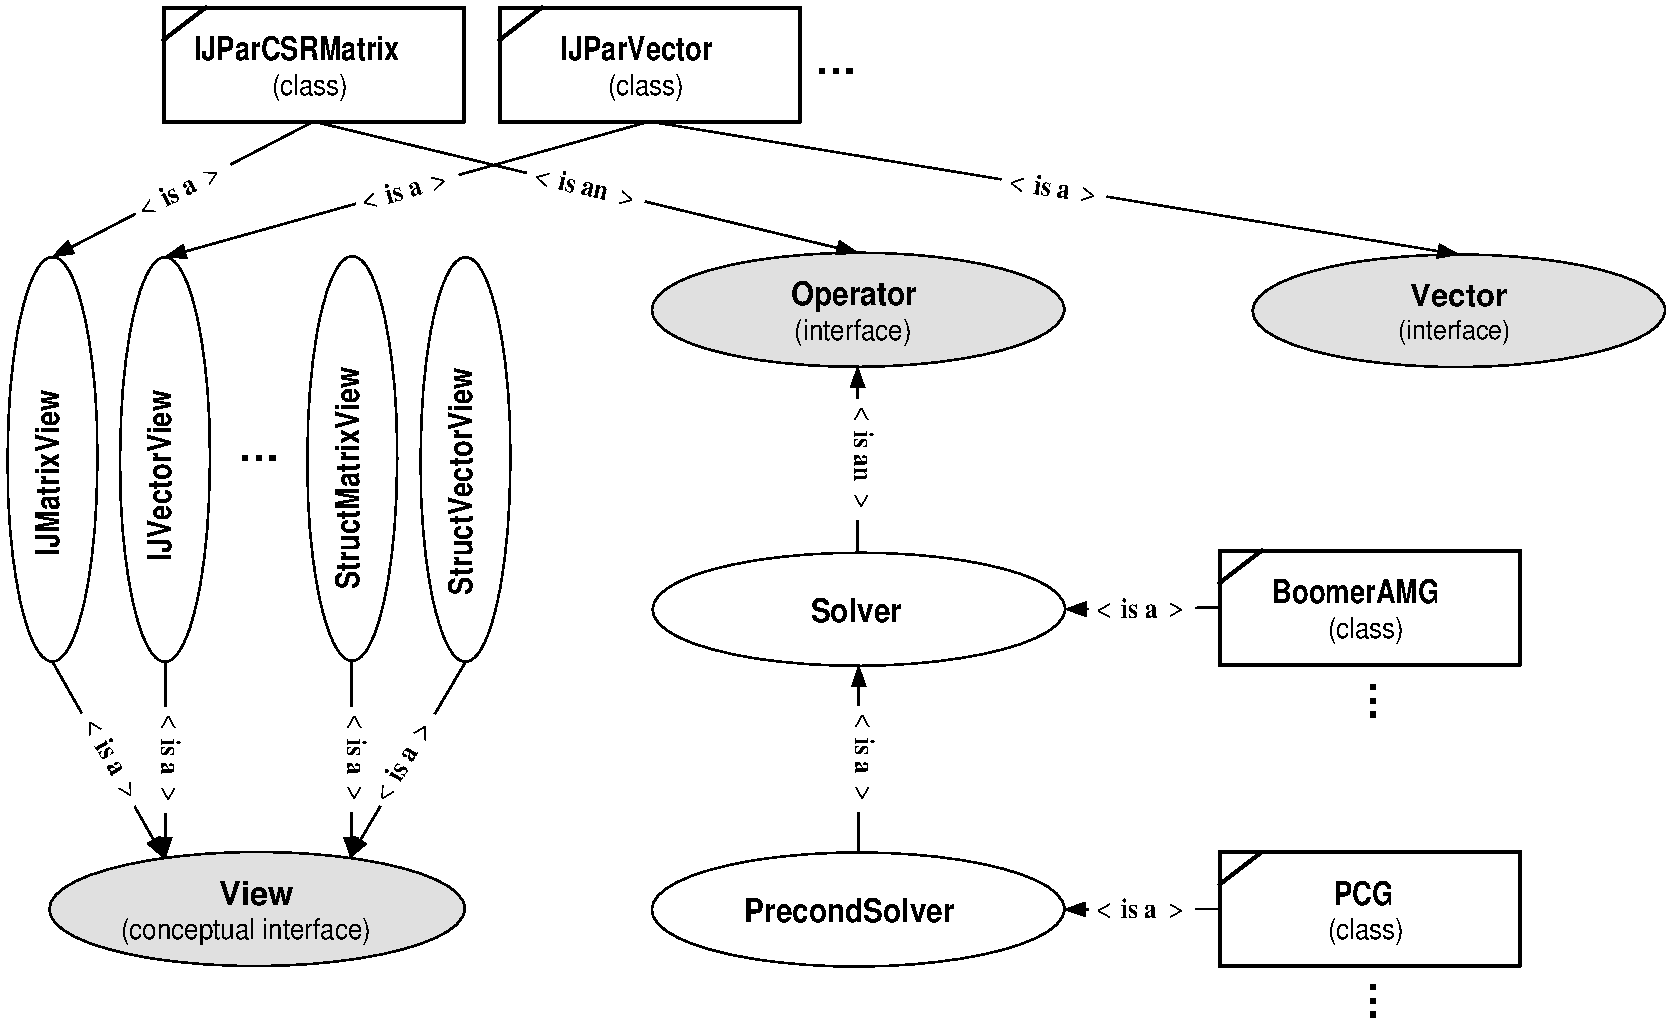
\includegraphics[width=5in]{figObjectModel}
\caption{%
The ideas of the hypre object model.}
\label{figObjectModel}
\end{figure}

% The same chart appears in the following two places, among others.
% 1. page 5 of ``The Design and Implementation of hypre, a Library of
% Parallel High Performance Preconditioners''
% (jfp has this in an email from Rob Falgout on May 13, 2005)
% 2. slide 79 of ACTS viewgraphs on hypre dated August 23, 2005 (jfp
% has this in an email from Rob Falgout dated July 19, 2006)


% >>>>>>> a more complete chart would be nice, if it would fit! <<<<<<<<

% >>>>>>> a verbal description of the object system, e.g. what is a
% view, is ESSENTIAL ! <<<<<<<<<
% concepts to include:
% conceptual interface (e.g. IJ) vs 'underlying storage type' (e.g. ParCSR)

\section{Arrays}
\label{sec-Arrays}

Almost always, when you pass an array through the Babel-based
interface, you do it in the natural way - you build and use the array
type which is native to your language.  Babel calls this kind or array
a ``raw array'' or ``rarray.''  In \hypre{}, they are
one-dimensional too.  It is usually obvious how to use them.

Just two functions in \hypre{}, \code{GetRow} and
\code{CoefficentAccess}, require a special type of array, which Babel
calls a ``SIDL array.''  This has more structure than the arrays
native to languages like C or Fortran - it accomodates reference
counting and knows its own size, for example.

The following examples show a way to declare, read, and destroy a SIDL
array.  The GetRow and CoefficentAccess functions create their output
arrays, so there is no need to create your own.  For more information
on these arrays, read the Babel documentation at
\url{http://www.llnl.gov/CASC/components}.

% I've never done any of this.  This should be put in the test
% programs sometime.

\subsubsection{C}
\begin{verbatim}
    struct sidl_int__array *row_js;
    struct sidl_double__array *row_data;
    bHYPRE_IJParCSRMatrix_GetRow( A, i, &row_size, &row_js, &row_data, ex );
    for ( k=0; k<row_size; ++k )
       col[k]  = sidl_int__array_get1( row_js, k );
       data[k] = sidl_double__array_get1( row_data, k );
    sidl_int__array_deleteRef( row_j, ex );
    sidl_double__array_deleteRef( row_data, ex );
\end{verbatim}
\subsubsection{Fortran}
\begin{verbatim}
      integer*8 row_js;
      integer*8 row_data;
      call bHYPRE_IJParCSRMatrix_GetRow_f( A, i, row_size, row_js,
     1                                     row_data, ex )
      do k = 1, row_size
         call sidl_int__array_get1_f( row_js, k-1, col(k) )
         call sidl_double__array_get1_f( row_data, k-1, data(k) )
      enddo
      call sidl_int__array_deleteRef( row_j, ex )
      call sidl_double__array_deleteRef( row_data, ex )
\end{verbatim}


\section{Building HYPRE with the Babel Interface}
\label{sec-Building-Babel}

You can build \hypre{} almost the same way with and without the
Babel-based interface.  Normally the only difference is that the
configure line needs an extra argument; for example:

\begin{verbatim}
    configure --with-babel
    make
\end{verbatim}
rather than
\begin{verbatim}
    configure
    make
\end{verbatim}

The configure system will enable whatever built-in languages it can
find compilers for.

The configure system for the runtime portion of Babel (included with
\hypre{} and enabled with the Babel-based interface) will
automatically compile and run a few tiny test programs.  This has been
a problem in multiprocessing AIX systems, where compiled programs are
normally run in a different environment from the configure system.
For AIX systems with POE, the
\hypre{} distribution includes a workaround script, \code{nopoe}.
When necessary, build \hypre{} as follows instead of the above:

\begin{verbatim}
    nopoe configure --with-babel
    make
\end{verbatim}

% I could write something about how building interfaces to other
% languages, but that may be too advanced for a user manual.

\subsection{Building HYPRE with Python Using the Babel Interface}
\label{sec-Building-Babel-Python}

To build the hypre library so you can call it from Python code, the
first step is to build a suitable Python!  Start with a recent version
of Python with the Numeric Python extension; for details see the
section on recommended external software in the Babel Users' Manual.

We have only tested hypre's Python interface with pyMPI, a Python
extension which supports MPI.  It is likely that you can make it work
with other MPI extensions, or even no MPI at all.  If you try this,
let us know how it works.

You will need write access to your Python's site-packages directory.
When you install pyMPI it creates another instance of Python, so this
should not be a problem.

You must configure and build hypre with shared libraries, because
Python requires them.  And specify what Python you are building for;
files will be written into its site-packages directory.
For example:
\begin{verbatim}
  configure --with-babel --enable-shared --enable-python=pyMPI
  make
\end{verbatim}

Finally, you need to set two environment variables.
\code{LD_LIBRARY_PATH} must include the path to the hypre shared
libraries, e.g. \code{src/hypre/lib}.
\code{SIDL_DLL_PATH} must include the path to an
\code{.scl} file generated for the Python interface,
e.g.\begin{verbatim}
src/babel/bHYPREClient-P/libbHYPRE.scl
\end{verbatim}
If you are running multiple processes, these environment variables may
need to be set in a dotfile so all processes will use the same values.

See the examples directory for an example of how to write a Python
program which uses hypre.


%--------------- Include Other

% \input{glossary}

%--------------- Print the References here

\bibliographystyle{plain}
\bibliography{hypre}

%--------------- Print the Index here

%\printindex

\end{document}


